\documentclass{./packages/homework}
\usepackage{./packages/caratula}
\usepackage{amssymb}
\usepackage{graphicx}
\usepackage{caption}

\graphicspath{./files/src/media/}
\renewcommand{\contentsname}{contenidos}
\renewcommand{\refname}{Referencias}
\renewcommand\qedsymbol{$\blacksquare$}
\renewcommand{\lstlistingname}{Algoritmo}% Listing -> Algorithm
\renewcommand{\figurename}{Figura}% Listing -> Algorithm
\renewcommand\thesubfigure{\roman{subfigure}}
\captionsetup[subfloat]{labelformat=empty}

\lstdefinelanguage{pseudo}{
  morekeywords={
    pre,
    post,
    if,
    while,
    for,
    in,
    out,
    proc,
    inout,
    do,
    and,
    not,
    return,
    break,
    raise
  },
  sensitive=false, % keywords are not case-sensitive
  morecomment=[l]{//}, % l is for line comment
  morecomment=[s]{/*}{*/}, % s is for start and end delimiter
  keywordstyle=\color{black}\textbf,
  commentstyle=\color{gray},
  morestring=[b]", % defines that strings are enclosed in double quotes
  inputencoding=utf8,
  extendedchars=true,
  literate=
    {λ}{$\lambda$}1
    {α}{$\alpha$}1
    {ε}{$\epsilon$}1
    {Λ}{$\Lambda$}1
    {>=}{$\geq$}2
    {<=}{$\leq$}2
}

\newcommand{\TODO}[1]{
  {\noindent \color{red} [#1]}
}



\begin{document} 

% caratula
\titulo{TP 2: Análisis de Redes Sociales}
\subtitulo{}
\fecha{Octubre 27, 2022}
\materia{Métodos Numéricos}
\grupo{Grupo 18}

\integrante{Vekselman, Nat\'an}{338/21}{natanvek11@gmail.com}
\integrante{Arienti, Federico}{316/21}{fa.arienti@gmail.com}
\integrante{Manuel Lakowsky}{511/21}{mlakowsky@gmail.com}
\integrante{Brian Kovo}{1218/21}{brian.ilank@gmail.com}

\maketitle


% palabras clave y resumen
\addtocontents{toc}{\protect\setcounter{tocdepth}{0}}
\section*{resumen}
\addtocontents{toc}{\protect\setcounter{tocdepth}{2}}
La descomposición de matrices en autovectores y autovalores aparece en una variedad de aplicaciones donde importa caracterizar el comportamiento de un sistema. Por ejemplo, en el reconocimiento de imágenes o en el análisis de redes. Desde un punto de vista geométrico, se puede considerar a los autovectores como los `ejes' de una transformación lineal, en tanto representan una dirección invariante a la transformación, y a los autovalores como los factores por los que esas direcciones se comprimen, estiran o invierten. 

\vspace{1em}
En este trabajo propondremos una implementación en C++ de un método para el cálculo de autovalores y autovectores en matrices cuadradas. Para algunas matrices particulares, como pueden ser las matrices simétricas definidas positivas, este método nos permitirá obtener todos sus autovalores y autovectores asociados. El mismo se conoce como \textit{el método de la potencia con deflación}. 

A su vez, presentaremos dos aplicaciones concretas de los autovalores y autovectores en el análisis de redes: la medición de centralidad de autovector y corte mínimo en la red del \textit{`Club de Karate'} \cite{Zachary}, y la estimación de una \textit{ego-network} \cite{Leskovec} de Facebook, por medio de la construcción de una matriz de similaridad.  

\vspace{1em}
\noindent Palabras clave: \textit{método de la potencia, deflación de Hotelling, centralidad de autovector, conectividad algebráica, análisis de componentes principales.}

% \newpage
\vspace{2em}

% contenido
\tableofcontents
\newpage

% potencia
\section{Método de la potencia con deflación}
% === INTRO === %

\vspace{1em}
\subsection{Introducción teórica} El método de la potencia con deflación permite aproximar un subconjunto de los autovalores y autovectores asociados a una matriz. Si la misma satisface que todos sus autovalores son no nulos y diferentes en módulo, entonces permite aproximar el conjunto entero. 


\vspace{2em}
\noindent \textsc{Método de la potencia}. El método de la potencia, \textit{Power method} o \textit{Power iteration}, es una técnica iterativa para aproximar el autovector asociado al autovalor en módulo máximo de una matriz cuadrada que satisfaga esta característica ---es decir, tenga un autovalor dominante no nulo---, a partir de la aplicación de sucesivos productos matriciales, descriptos por la siguiente relación de recurrencia:

\begin{equation} \label{potencia}
    b_{k+1} = \frac{\mathbf{A}b_k}{||\mathbf{A}b_k||} \qquad \forall k \in \mathbf{N}_0
\end{equation}

\vspace{1em}
\noindent donde $b_0$ es un vector aleatorio, $||b_0|| = 1$ y $|| \cdot ||$ es una norma vectorial.

\vspace{1em}
Se puede demostrar \cite{Burden} que, bajo las condiciones descriptas, si k es par y $b_0$ no es ortogonal al autovector asociado al autovalor en módulo dominante de \textbf{A}, entonces $b_k$ siempre convergerá a éste\footnote{De manera más formal, la secuencia definida por $\{b_k\}_{k \in \mathbb{N}_0}$ es acotada para $k$ y $\lambda_{max}$ arbitrarios, pero la subsecuencia definida para $k$ par es absolutamente convergente.}. Lo que es más, se podrá aproximar el autovalor dominante por medio del coeficiente de Rayleigh:

\vspace{1em}
\begin{equation} \label{rayleigh}
    \lambda_{max} = \frac{b_k^t\ \mathbf{A}\ b_k}{b_k^t\ b_k}
\end{equation}


\vspace{2em}
\noindent \textsc{Método de la deflación}. El método de la deflación, por su parte, corresponde a la transformación de la matriz inicial \textbf{A} por una matriz \textbf{B} con autovalores equivalentes, salvo por el autovalor dominante que será anulado. Existen distintos métodos de deflación, entre ellos la deflación de Hotelling y la deflación de Wielandt \cite{Burden}.  

En este trabajo utilizaremos la deflación de Hotelling por su sencillez, a cuestas de un mayor error numérico \cite{Burden}. La misma consiste en aplicar el método de la potencia para sucesivas matrices que satisfagan la siguiente relación:

\vspace{1em}
\begin{equation} \label{deflacion}
    \mathbf{B}_{k+1} = \mathbf{B}_{k} - \lambda_k\ v_k\ v_k^t \qquad \forall k \in \mathbf{N}_0
\end{equation}

\vspace{2em}
\noindent donde $\mathbf{B}_0 = \mathbf{A}$, $\lambda_k$ corresponde al k-ésimo autovalor en módulo máximo de \textbf{A}, estimado por el método de la potencia, y $v_k$ es su autovector asociado.

%\vspace{1em}
%Se puede demostrar que $\mathbf{B}_{k+1}$ contiene los mismos autovalores que $\mathbf{B}_{k}$, salvo el máximo que quedará anulado.




% === IMPLEMENTACION === %

\vspace{2em}
\subsection{Implementación} Procedemos a detallar una posible implementación\footnote{El código se puede encontrar en \textit{./implementacion/src/}.} para ambos métodos, restringiéndonos al caso de autovalores reales. Definimos:

\begin{align*}
    \text{\textit{deflacion}}&:\ \text{\textit{matriz}}_{n \times n}\ \mathbf{A}\ \times\ \text{\textit{nat} k}\ \times\ \text{\textit{nat} q}\ \times\ \text{\textit{real} t}\
    \longrightarrow\ \text{\textit{vector}}_k\ \times\ \text{\textit{matriz}}_{n \times k}
    \\ \\
    \text{\textit{potencia}}&:\ \text{\textit{matriz}}_{n \times n}\ \mathbf{A}\ \times\ \text{\textit{nat} q}\ \times\ \text{\textit{real} t}\ 
    \longrightarrow\ \text{\textit{real}}\ \times\ \text{\textit{vector}}_n
\end{align*}

\vspace{1em}
\noindent donde $n$ es un natural, \textbf{A} tiene al menos $k$ autovalores reales dominantes en módulo, $0 < k \leq n$, $q$ es un número par\footnote{Esta restricción no es necesaria, pero permite mantener exacta la cantidad de iteraciones a realizar.} que representa el máximo de iteraciones a realizar y $0 \leq t$ representa la tolerancia mínima a partir de la que se considera la convergencia de una solución. 

\vspace{1em}
\lstinputlisting[mathescape=true, escapechar=@, language=pseudo, label=algo_deflacion, caption={Pseudocódigo para el método de la deflación.}]{files/src/.code/deflacion.pseudo}

%\vspace{1em}
El algoritmo (\ref{algo_deflacion}.) retornará un vector con los primeros $k$ autovalores en módulo máximos de \textbf{A}, ordenados descendientemente, y una matriz cuyas columnas corresponden, respectivamente, a los autovectores normalizados asociados a estos autovalores. 

\vspace{1em}
Es interesante notar que la $k$-ésima matriz sobre la que se aplicará el método de la potencia ---\textbf{B}$_k$--- tendrá, por definición, un autovalor cero con multiplicidad algebraica mayor o igual a $k$. En el caso en que la matriz inicial sea simétrica, \textbf{B}$_k$ será simétrica\footnote{Por suma de simétricas. Notar que $v v^t$ siempre resulta en una matriz de este tipo.} y, en consecuencia, diagonalizable. Se puede demostrar que la única matriz diagonalizable con multiplicidad algebraica $\mu_{a}(0) = n$ es la matriz nula, por lo que el método de la deflación de Hotelling tenderá hacia ella. Esto nos permite inferir que el error numérico será proporcional a $k$\footnote{En tanto existirá una correlación. Sin embargo, es esperable que otros factores entren en juego: la varianza de los autovalores, el número de condición de la matriz, la selección del vector aleatorio inicial, o la cantidad de iteraciones $q$ a realizar, por ejemplo.}. Es decir, los autovalores más chicos de la matriz serán más susceptibles a errores.  


\vspace{2em}
\noindent Por su parte, el algoritmo (\ref{algo_potencia}.) retornará el autovalor de \textbf{A} máximo en módulo y su autovector asociado:

\vspace{1em}
\lstinputlisting[mathescape=true, escapechar=@, language=pseudo, caption={Pseudocódigo para el método de la potencia \textit{monte carlo}.}, label=algo_potencia]{files/src/.code/potencia.pseudo}

\vspace{1em}
Observamos que el algoritmo (\ref{algo_potencia}.) trabaja con la subsecuencia par de $\{b_k\}_{k \in \mathbb{N}_0}$. Como mencionamos antes, esto garantiza la convergencia absoluta del método, dada una selección inicial de $b_0$ ---$v$ en nuestro pseudocódigo--- no ortogonal al autovector asociado al autovalor en módulo dominante\footnote{Para ver un análisis en más detalle, ver la experimentación (\ref{ap_A}.).}. Sin embargo, como esta selección depende de un proceso aleatorio, el algoritmo podrá resultar en una respuesta incorrecta. A este tipo de procesos se los denomina \textit{monte carlo} \cite{Brassard}. 

\vspace{1em}
Una variante posible, de tipo \textit{las vegas}, se presenta en el algoritmo (\ref{algo_potencia_vegas}.). Hasta llegar a un resultado aceptable, determinado por $\epsilon$, o superar la cantidad de iteraciones permitida, definida por $\alpha$, el algoritmo volverá a intentar resolver el problema. De no alcanzar una respuesta aceptable retornará una señal de error. 

De este modo, la probabilidad de fallar a causa de una selección inicial ortogonal al autovector al que se espera converger será inversamente proporcional a $\alpha$\footnote{Esto es, considerando que cada selección inicial es independiente.}. 

\vspace{1em}
Para reducir esta probabilidad desde el comienzo, se propone que se elija cada coordenada del vector de manera pseudo-aleatoria sobre un rango amplio\footnote{Desde un punto de vista geométrico, dos vectores son ortogonales sólo si son perpendiculares. De manera intuitiva, podemos ver que a medida que la dirección inicial posible de un vector tiende al infinito, la probabilidad que forme un ángulo de 90 grados con otro tiende a cero.}. Por ejemplo, la máxima representación de enteros con signo en 32 bits. 

\vspace{1em}
\lstinputlisting[mathescape=true, escapechar=@, language=pseudo, caption={Pseudocódigo para el método de la potencia \textit{las vegas}.}, label=algo_potencia_vegas]{files/src/.code/potencia_vegas.pseudo}

\vspace{1em}
Es importante mencionar que una mala selección de $\epsilon$ ---en función de $q$ y $t$--- resultará en un algoritmo que siempre falla. Esto dependerá de la velocidad de convergencia del método para la matriz particular sobre la que se lo aplica.  




% === EVALUACION === %
\vspace{2em}
\subsection{Evaluación cuantitativa} Procedemos a realizar una evaluación de nuestra implementación en C++ acorde a los algoritmos propuestos\footnote{El script asociado se puede encontrar en \textit{./experimentos/error\_potencia.py}, las tablas resultantes en \textit{./experimentos/resultados/error-potencia}.}. Se optó por utilizar el método de la potencia \textit{monte carlo}.

\vspace{1em}
\noindent Medimos el error relativo $\ ||\mathbf{A} \mathbf{\bar{V}} - \mathbf{\bar{V}} \mathbf{\bar{\Lambda}}||\ $ y absoluto $\ ||\mathbf{\Lambda} - \mathbf{\bar{\Lambda}}||\ $ para 300 instancias de matrices $\mathbf{A} \in \mathbb{R}^{20 \times 20}$ generadas aleatoriamente, donde $\mathbf{\bar{V}}$ y $\mathbf{\bar{\Lambda}}$ representan, respectivamente, las matrices aproximadas de autovectores y autovalores de \textbf{A}.


\vspace{2em}
\noindent \textsc{Metodología}. Se calculó $\mathbf{\bar{\Lambda}}, \mathbf{\bar{V}} = \text{\textit{deflacion}}(\mathbf{A},\ 20,\ 2e^4,\ 1e^{-20})$ y se midió el error relativo y absoluto del resultado.

\vspace{1em}
\noindent Cada caso se generó a través de uno de los siguientes tres procedimientos\footnote{Se utilizó un valor semilla para facilitar la reproductibilidad.}:

\vspace{1em}
\begin{enumerate}
    \item \textit{Matrices Diagonales}: Se generaron cien matrices diagonales \textbf{D} con cien autovalores en el rango $[-1e^3, 0)\ \cup\ (0,\ 1e^3]$, con paridad diferente acorde al signo\footnote{De esta manera se garantiza la dominancia estricta en módulo de los autovalores asociados a la matriz.}. Los mismos se generaron con el rng \textit{PCG64} de numpy.
    \\
    \item \textit{Matrices Diagonalizables}: Se generaron cien matrices diagonalizables $\mathbf{A} := \mathbf{Q} \mathbf{D} \mathbf{Q}^t$ donde cada matriz $\mathbf{D}$ se generó a partir de la metodología (1.) y $\mathbf{Q} := \mathbf{I} - 2uu^t$ se generó a partir de un vector aleatorio $u$ ---con el algoritmo \textit{random.rand()} de numpy--- tal que $||u||_2 = 1$.
    \\
    \item \textit{Matrices Simétricas Definidas Positivas}: Se generaron cien matrices simétricas definidas positivas de enteros $\mathbf{A} := \mathbf{B} \mathbf{B}^t$ donde \textbf{B} es una matriz aleatoria generada con el algoritmo \textit{random.randint()} de numpy para el rango $[-1e^3, 0)\ \cup\ (0,\ 1e^3]$.
\end{enumerate}

\vspace{2em}
\noindent \textsc{Observaciones}. Consideramos que la varianza de los autovalores, el número de condición de las matrices, y su tamaño, son variables que afectan de manera significativa en el error del procedimiento. 

El proceso mencionado para la generación de matrices aleatorias fue pensado sobre generadores de números aleatorios para tratar de minimizar cualquier tendencia que pueda provenir de la utilización de distribuciones particulares. De esta manera se espera que la varianza de los autovalores y el número de condición de las matrices también sean aleatorios, tal que los resultados brinden un panorama amplio del dominio de aplicación del método propuesto. 

Además, se controló el tamaño de $n$, la cantidad de iteraciones $q$ y la tolerancia $t$. Un estudio más exhaustivo debería también evaluar el comportamiento del algoritmo en función de estos parámetros.

\vspace{2em}
\noindent \textsc{Resultados}. La Figura (\ref{error_relativo}.) resume los resultados para el error relativo.

\vspace{1em}
\begin{figure}[!htbp]
    \begin{tabular}{ |l|c|c| } 
    \hline
    test                    & $L_1$             & $L_\infty$ \\
    \hline
    mediciones              & 300               & 300 \\
    error relativo promedio & $2.20e^{-3}$  & $3.69e^{-4}$ \\
    desviación estándar     & $3.36e^{-2}$  & $5.83e^{-3}$ \\
    mínimo                  & 0.0               & 0.0 \\
    25\%                    & 0.0               & 0.0 \\
    50\%                    & $2.00e^{-11}$ & $1.01e^{-11}$ \\
    75\%                    & $4.13e^{-6}$  & $7.97e^{-7}$ \\
    máximo                  & $5.81e^{-1}$  & $1.01e^{-1}$ \\
    \hline
    \end{tabular} \\
    \bigskip
    \caption{Datos de resumen para el error relativo $||\mathbf{A} \mathbf{\bar{V}} - \mathbf{\bar{V}} \mathbf{\bar{\Lambda}}||$.} \label{error_relativo}
\end{figure}

\vspace{1em}
\noindent La Figura (\ref{error_absoluto}.), por su parte, resume los resultados para el error absoluto.

\vspace{1em}
\begin{figure}[!htbp]
    \begin{tabular}{ |l|c|c| } 
    \hline
    test                    & $L_1$             & $L_\infty$ \\
    \hline
    mediciones              & 300               & 300 \\
    error relativo promedio & $3.43e^{-7}$  & $2.05e^{-7}$ \\
    desviación estándar     & $5.05e^{-6}$  & $3.31e^{-6}$ \\
    mínimo                  & 0.0               & 0.0 \\
    25\%                    & 0.0               & 0.0 \\
    50\%                    & $2.20e^{-12}$ & $4.55e^{-13}$ \\
    75\%                    & $1.31e^{-7}$  & $2.98e^{-8}$ \\
    máximo                  & $8.75e^{-5}$  & $5.73e^{-5}$ \\
    \hline
    \end{tabular} \\
    \bigskip
    \caption{Datos de resumen para el error absoluto $||\mathbf{\Lambda} - \mathbf{\bar{\Lambda}}||$.} \label{error_absoluto}
\end{figure}

\vspace{1em}
Vemos que el método funcionó, para el 75\% de las matrices evaluadas, con un error relativo y absoluto menor a $1e^{-4}$. Sin embargo, notamos que existen casos anómalos para los que el error puede ser mayor.

Por la disparidad entre el error relativo y absoluto, podemos inferir ---a modo de futura hipótesis a investigar--- que el método produce más error en los autovectores resultantes que en los autovalores.

\newpage

% club de karate
\section{Análisis: Club de Karate}
% === CONTEXTO === %

\vspace{1em}
\subsection{Contexto}

La red del \textit{Club de Karate} fue parte de una investigación antropológica \cite{Zachary}, realizada por Wayne W. Zachary, que estudió las relaciones `políticas' entre los miembros de un club universitario. La misma se realizó durante el desarrollo de un conflicto que terminó por dividir al grupo. 

La red buscó modelar el flujo de información entre sus integrantes por medio de la tripla $(\mathbf{V},\ \mathbf{E},\ \mathbf{C})$, donde $\mathbf{V}$ denota el conjunto de individuos, $\mathbf{E}$ refiere a un grafo no direccionado cuyos ejes representan los vínculos entre los miembros del club, y $\mathbf{C}$ define la fuerza de estas relaciones ---lo que se podría pensar como ponderaciones sobre los ejes de $\mathbf{E}$---. 

\vspace{1em}
La investigación tuvo como enfoque central demostrar la capacidad del modelo para predecir la división del grupo por medio del algoritmo de \textit{labeling} de `flujo máximo - corte mínimo' de Ford y Fulkerson \cite{Ford}.

\vspace{1em}
\begin{figure}[!htbp]
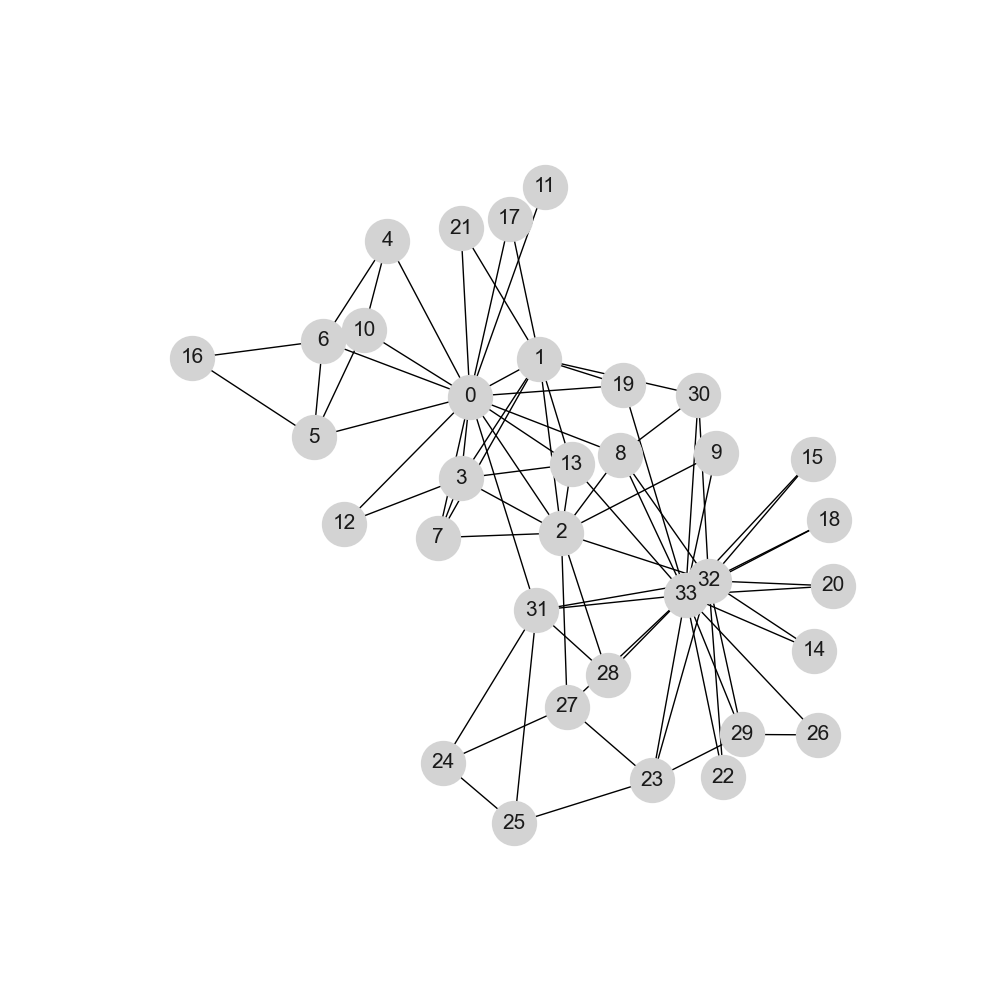
\includegraphics[scale=0.55, trim=100 80 100 100, clip]{/files/src/.media/karate/grafo_conectividad.png}
\caption{La red del \textit{Club de Karate}. Cada nodo representa un individuo, cada eje la existencia de un vínculo por fuera del club.}
\end{figure}


\vspace{1em}
En este análisis\footnote{El script asociado se puede encontrar en \textit{./experimentos/club\_de\_karate.py}, los archivos con los resultados en \textit{./experimentos/resultados/club-karate/}.} utilizaremos la representación matricial de $\mathbf{E}$ para evaluar la importancia de los distintos miembros en la red, y la matriz laplaciana asociada para evaluar el uso de autovectores como predictores de la división del grupo. 

 


% === CENTRALIDAD DE AV === %
\newpage
\vspace{2em}
\subsection{Centralidad de Autovector} La centralidad de autovector es una medida que se utiliza en el análisis de redes para evaluar la `importancia' de los nodos que componen una red, relativa a la importancia de sus conexiones. Dada una matriz de conectividad $\mathbf{W} \in \mathbb{R}^{n \times n}$, se define:

\vspace{1em}
\begin{equation} \label{conectividad}
    \lambda x = \mathbf{W} x
\end{equation}

\vspace{1em}
\noindent donde $\lambda$ es el autovalor en módulo máximo de \textbf{W} y la coordenada $x_i$ ---del autovector $x$ asociado a $\lambda$--- denota la centralidad del nodo $i$, $\forall i:\ 1\ ...\ n$.

\vspace{1em}
Intuitivamente, se puede pensar que la importancia de cada nodo es proporcional a la suma de las importancias de sus vecinos. Se puede demostrar \cite{Newman} que, dado las características de esta matriz, el autovector asociado tendrá el mismo signo en todas sus coordenadas.

\vspace{1em}
En tanto la red de \textit{Club de Karate}, podemos ver que la aplicación del método de la potencia sobre la matriz de conectividad asociada al grafo $\mathbf{E}$ resulta en el siguiente autovector $x$\footnote{Notamos que el error relativo del resultado fue de $\approx 7.81e^{-14}$ en norma $L_1$.}:

\vspace{1em}
\begin{figure}[!htbp]
\begin{equation*} 
    \begin{bmatrix}
        0   &0.355491 \\
        1   &0.265960 \\
        2   &0.317193 \\
        3   &0.211180 \\
        4   &0.075969 \\
        5   &0.079483 \\
        6   &0.079483 \\
        7   &0.170960 \\
        8   &0.227404 \\
        9   &0.102674 \\
        10  &0.075969 \\
        11  &0.052856 \\
        12  &0.084255 \\
        13  &0.226473 \\
        14  &0.101403 \\
        15  &0.101403 \\
        16  &0.023636 \\
    \end{bmatrix}
    \begin{bmatrix}
        17  &0.092400 \\
        18  &0.101403 \\
        19  &0.147913 \\
        20  &0.101403 \\
        21  &0.092400 \\
        22  &0.101403 \\
        23  &0.150119 \\
        24  &0.057052 \\
        25  &0.059206 \\
        26  &0.075579 \\
        27  &0.133477 \\
        28  &0.131078 \\
        29  &0.134961 \\
        30  &0.174758 \\
        31  &0.191034 \\
        32  &0.308644 \\
        33  &0.373363 \\
    \end{bmatrix}
\end{equation*}
\caption{Centralidad de autovector para la red del \textit{Club de Karate}. La columna izquierda denota el nodo, la derecha su `importancia'.} \label{centralidad_karate}
\end{figure}

\vspace{1em}
Vemos que el nodo `0' y el nodo `33' son los más centrales. Esto no es casualidad, la red del \textit{Club de Karate} está armada para tener a las dos figuras principales del conflicto en cada extremo ---el instructor de karate y el presidente del club, respectivamente--- para satisfacer la especificación del algoritmo de labeling que utiliza.




% === AV DE LA MATRIZ LAPLACIANA === %

\vspace{2em}
\subsection{Autovectores de la matriz laplaciana} La matriz laplaciana $\mathbf{L} = \mathbf{D} - \mathbf{W}$ ---donde \textbf{D} es una matriz diagonal con elementos $d_{ii} = \sum_j w_{ij}$ y \textbf{W} es una matriz de conectividad--- sirve para medir distintas propiedades en una red. 

En particular, el mínimo autovalor en módulo no nulo ---llamado de conectividad algebraica, o valor de Fiedler--- permite establecer un criterio sobre el que particionar la red en dos. El autovector asociado a este autovalor designará la pertenencia de un nodo a una u otra partición acorde a su signo. 

\vspace{1em}
Procedemos a analizar qué autovector de la matriz laplaciana asociada a $\mathbf{E}$ permite predecir mejor la división que ocurrió en el \textit{Club de Karate}. Para ello, calculamos los autovectores de la matriz con el método de la potencia con deflación\footnote{Notamos que el error relativo de los resultados tuvo una cota superior de $\approx 1.03e^{-13}$ en norma $L_1$.} y medimos el valor absoluto de la correlación entre cada autovector y un vector que indica la división verdadera que ocurrió en el grupo.

\vspace{1em}
\begin{figure}[!htbp]
\begin{equation*} 
    \begin{bmatrix}
        18.136696 & 0.045692 \\
        17.055171 & 0.011443 \\
        13.306122 & 0.078413 \\
        10.921068 & 0.058283 \\
        9.777241  & 0.085078 \\
        6.996197  & 0.010429 \\
        6.515545  & 0.079173 \\
        6.331592  & 0.014177 \\
        5.618034  & 0.0 \\
        5.378595  & 0.244844 \\
        4.580793  & 0.079869 \\
        4.480008  & 0.044972 \\
        4.275877  & 0.010777 \\
        3.472187  & 0.000321 \\
        3.381966  & 0.0 \\
        3.376154  & 0.065159 \\
        3.242067  & 0.086678 \\
    \end{bmatrix}
    \begin{bmatrix}
        3.013963 & 0.009556 \\
        2.749157 & 0.161363 \\
        2.487092 & 0.117379 \\
        2.0 & 0.0 \\
        2.0 & 0.0 \\
        2.0 & 0.0 \\
        2.0 & 0.0 \\
        2.0 & 0.0 \\
        1.955050 & 0.011172 \\
        1.826055 & 0.068783 \\
        1.761899 & 0.027133 \\
        1.599283 & 0.05576 \\
        1.259404 & 0.000408 \\
        1.125011 & 0.333307 \\
        0.909248 & 0.265918 \\
        0.468525 & 0.814727 \\
        0.0 & nan\footnotemark \\
    \end{bmatrix}
\end{equation*}
\caption{Correlación entre los autovectores asociados a los autovalores de la red del \textit{Club de Karate} y un vector que indica la división verdadera que ocurrió en el grupo. La columna izquierda denota el autovalor, la derecha la correlación.} \label{conectividad_karate}
\end{figure}
\footnotetext{El método de la potencia no está definido si el autovalor máximo en módulo es nulo. Este resultado da cuenta de ello. Como nos interesan solo los autovalores diferentes a `0', optamos por descartarlo.}

\vspace{1em}
Vemos que el valor de conectividad algebraica ---el autovalor mínimo en módulo no nulo--- tiene asociado el mejor autovector para realizar el corte. En la figura (\ref{prediccion_karate}.) se puede observar que sólo dos nodos obtuvieron una clasificación incorrecta: el `2' y el `8', lo que presenta un desempeño casi igual al logrado en la investigación original\footnote{En este sentido, solo el nodo `2' recibió una clasificación incorrecta. Sobre el `8', Zachary considera \cite{Zachary} que hubo un interés `egoísta' que primó sobre la `afiliación' política (es decir, las relaciones) del nodo.}.

\vspace{1em}
\begin{figure}[!htbp]
\begin{equation*}
    \begin{bmatrix}
        0   &-0.112137 & 0 & 0 \\ 
        1   &-0.041288 & 0 & 0 \\
        2   &0.023219  & 1 & 0 \\
        3   &-0.055500 & 0 & 0 \\
        4   &-0.284605 & 0 & 0 \\
        5   &-0.323727 & 0 & 0 \\
        6   &-0.323727 & 0 & 0 \\
        7   &-0.052586  & 0 & 0 \\
        8   &0.051601 & 1 & 0 \\
        9   &0.092801 & 1 & 1 \\
        10  &-0.284605  & 0 & 0 \\
        11  &-0.210993  & 0 & 0 \\
        12  &-0.109461  & 0 & 0 \\
        13  &-0.014742  & 0 & 0 \\
        14  &0.162751 & 1 & 1 \\
        15  &0.162751 & 1 & 1 \\
        16  &-0.422765  & 0 & 0 \\
\end{bmatrix}
\begin{bmatrix}
        17  &-0.100181  & 0 & 0 \\
        18  &0.162751 & 1 & 1 \\
        19  &-0.013637  & 0 & 0 \\
        20  &0.162751 & 1 & 1 \\
        21  &-0.100181  & 0 & 0 \\
        22  &0.162751 & 1 & 1 \\
        23  &0.155695 & 1 & 1 \\
        24  &0.153026 & 1 & 1 \\
        25  &0.160963 & 1 & 1 \\
        26  &0.187110 & 1 & 1 \\
        27  &0.127664 & 1 & 1 \\
        28  &0.095152 & 1 & 1 \\
        29  &0.167650 & 1 & 1 \\
        30  &0.073500 & 1 & 1 \\
        31  &0.098753 & 1 & 1 \\
        32  &0.130345 & 1 & 1 \\
        33  &0.118903 & 1 & 1 \\
    \end{bmatrix}
\end{equation*}
\caption{Autovector de Conectividad algebraica, la primer columna representa los nodos de la red, la segunda el autovector, la tercera la clasificación de cada nodo acorde a su signo y la cuarta la división verdadera que ocurrió.} \label{prediccion_karate}
\end{figure}

%\vspace{1em}
\begin{figure}[!htbp]
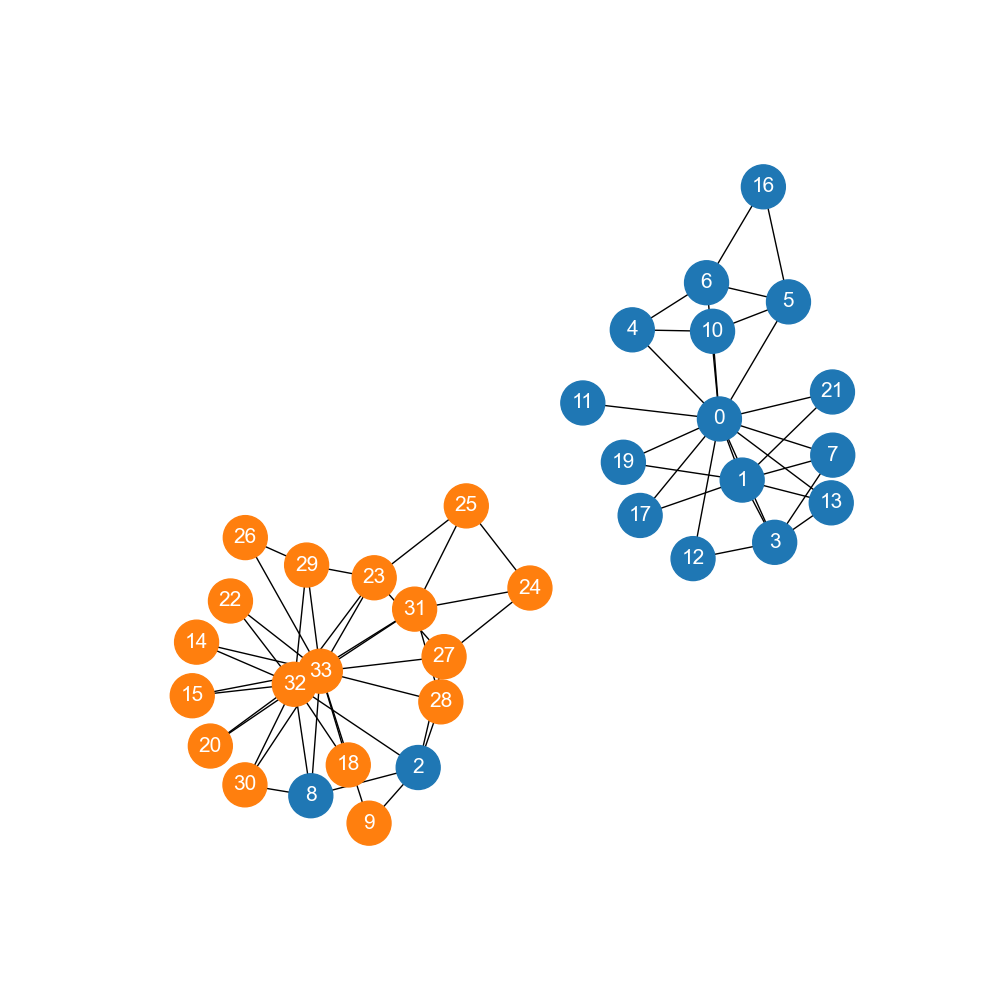
\includegraphics[scale=0.5, trim=100 90 100 100, clip]{/files/src/.media/karate/grafo_corte_32_0.47.png}
\caption{La división estimada de la red del \textit{Club de Karate}. Los colores representan la división verdadera de la red. Azul: `0', Naranja: `1'.}
\end{figure}

\vspace{1em}
Procedemos a detallar ---a modo de comparación visual--- los cortes realizados por los demás autovectores. Notamos que el proceso de corte sólo elimina los ejes existentes entre pares cuya clasificación difiere. Por ello, la cantidad de componentes conexos que puede generar un corte no es necesariamente dos.  

\begin{figure}[!htbp]
    \centering
    \subfloat[av $\approx$ 0.91]{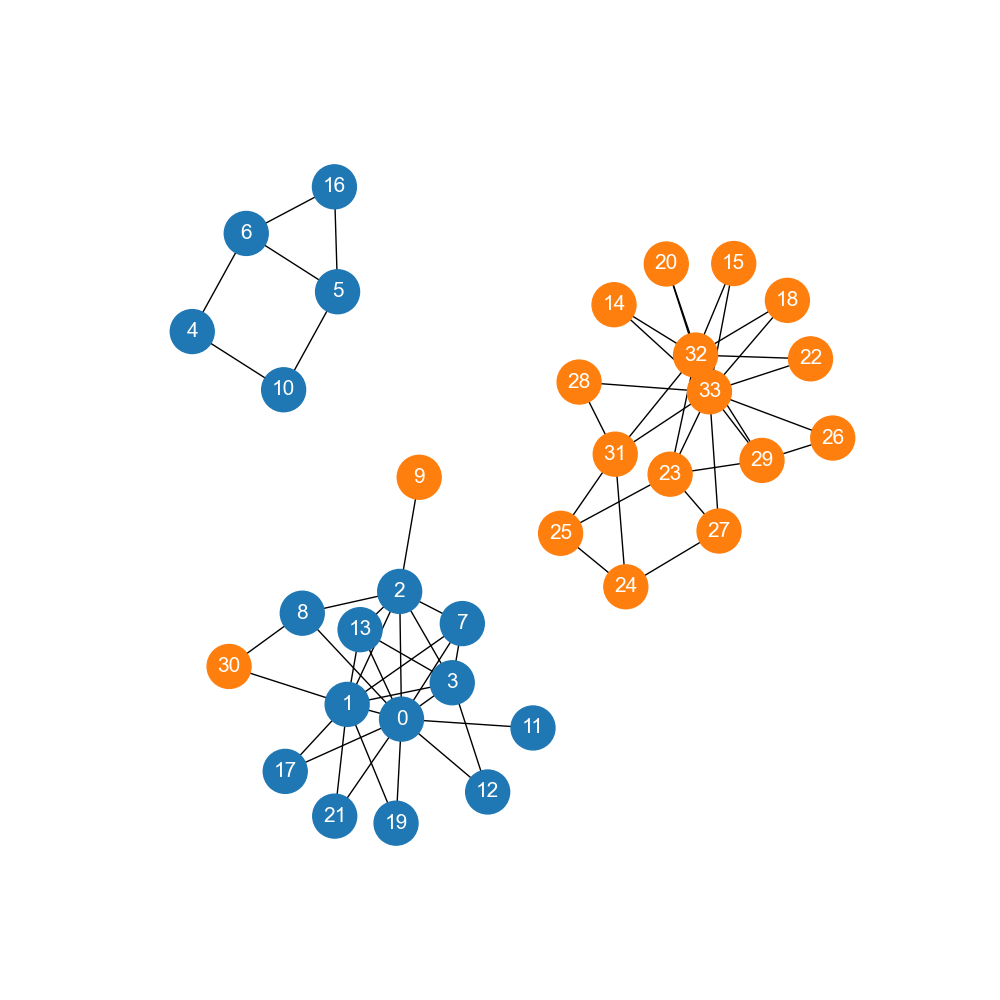
\includegraphics[width=.25\textwidth]{/files/src/.media/karate/grafo_corte_31_0.91.png}}\hfill
    \subfloat[av $\approx$ 1.13]{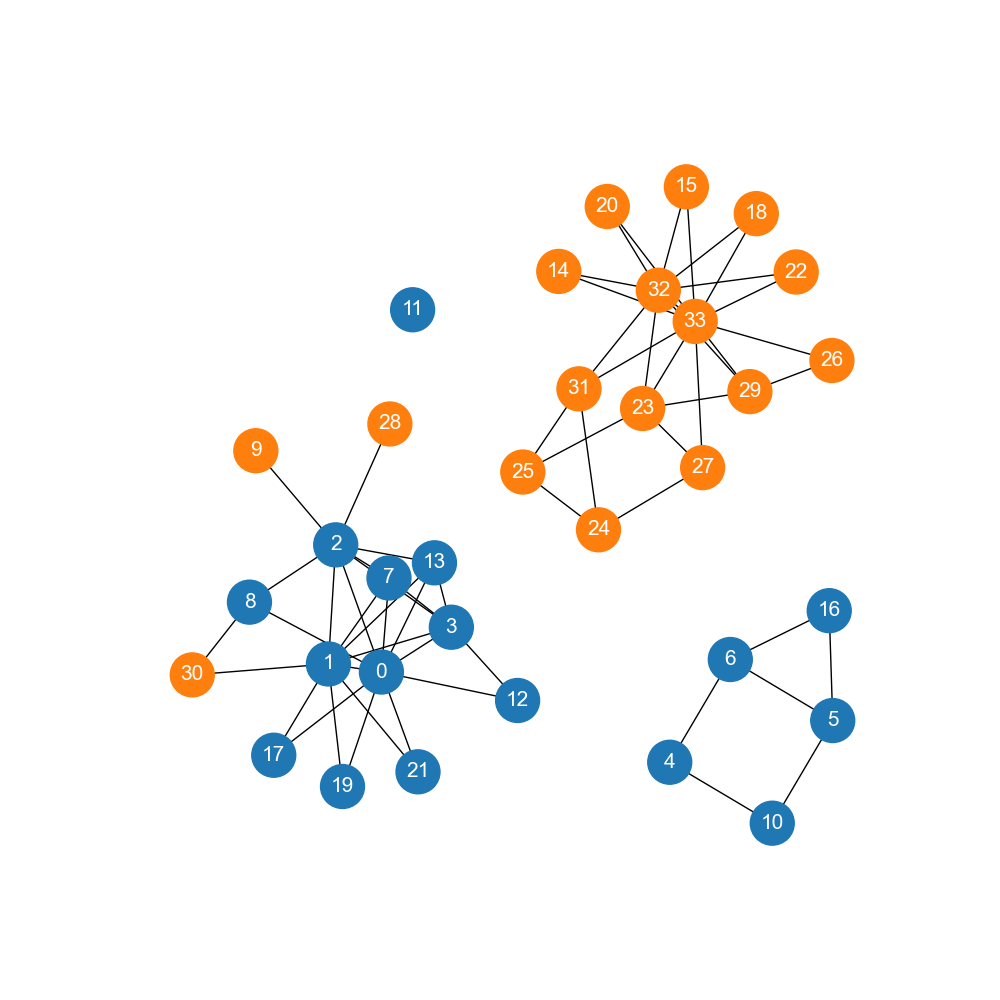
\includegraphics[width=.25\textwidth]{/files/src/.media/karate/grafo_corte_30_1.13.png}}\hfill
    \subfloat[av $\approx$ 1.26]{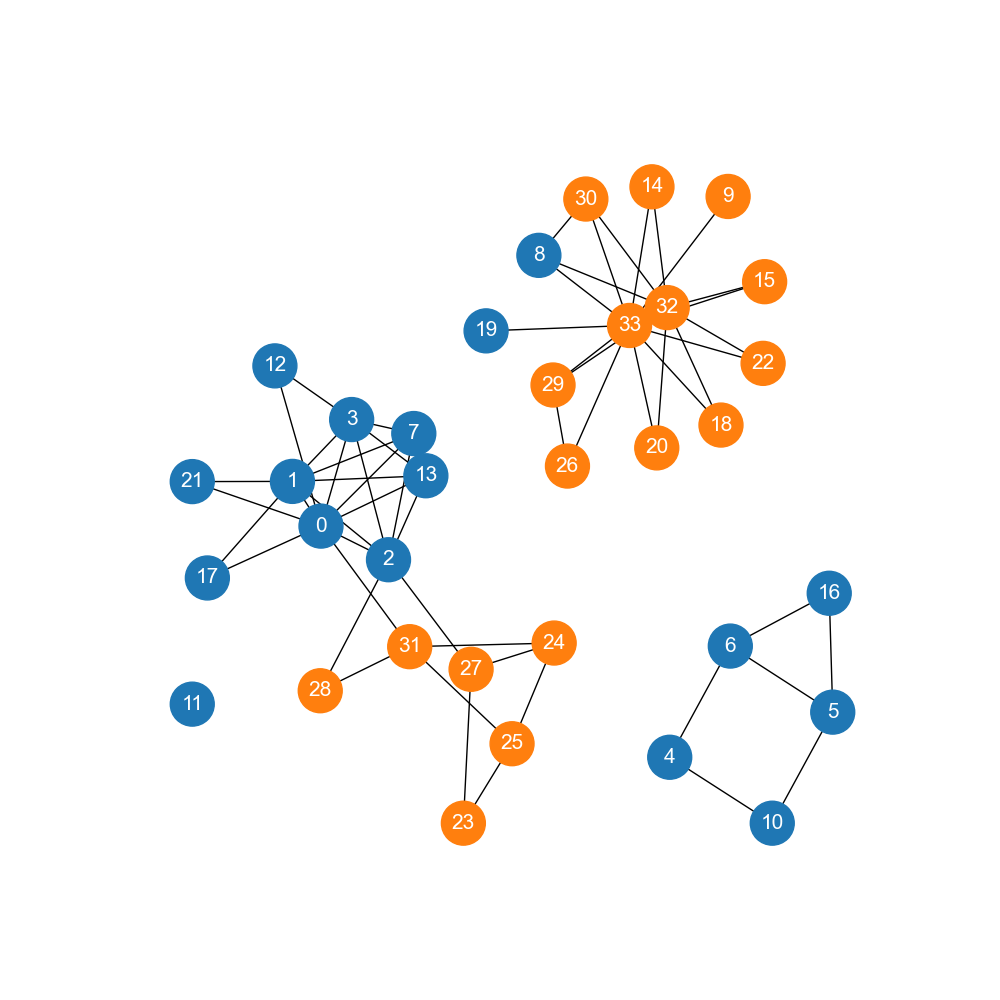
\includegraphics[width=.25\textwidth]{/files/src/.media/karate/grafo_corte_29_1.26.png}}\hfill
    \subfloat[av $\approx$ 1.60]{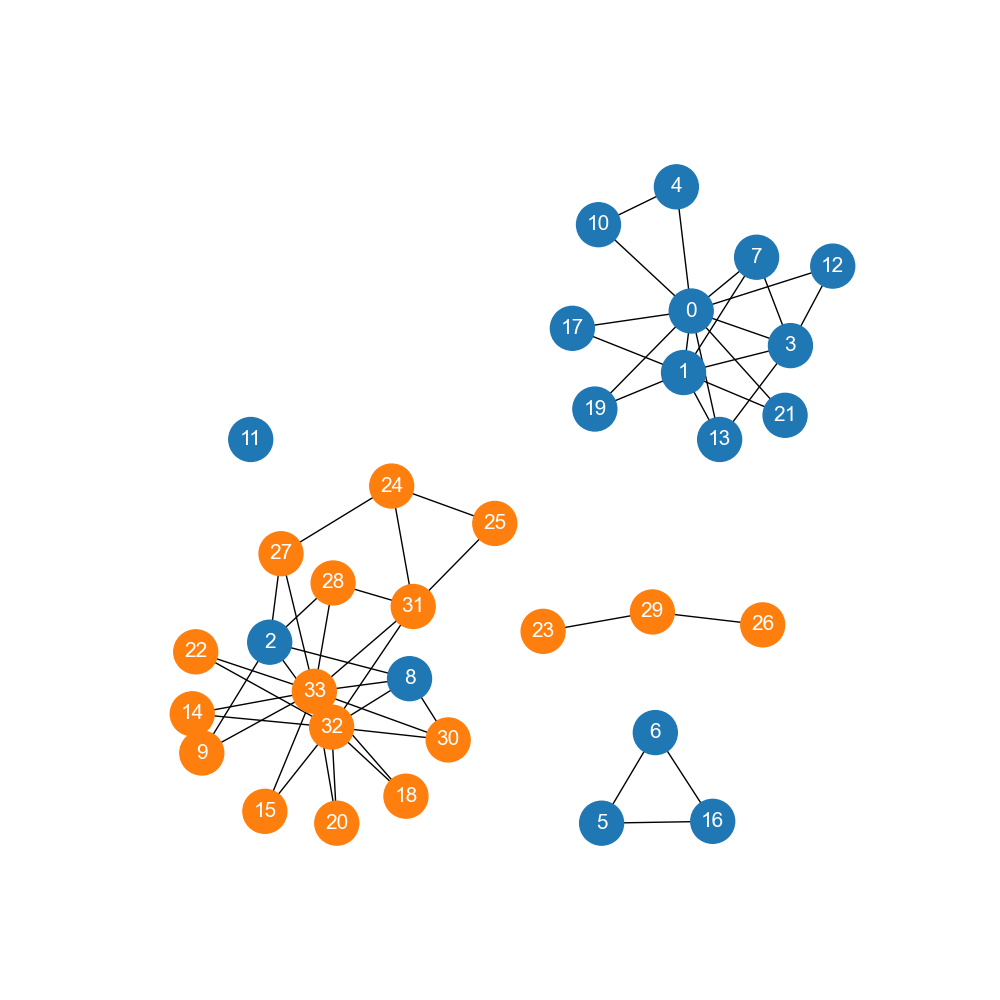
\includegraphics[width=.25\textwidth]{/files/src/.media/karate/grafo_corte_28_1.6.png}}\hfill
    \\[\smallskipamount]
    \subfloat[av $\approx$ 1.76]{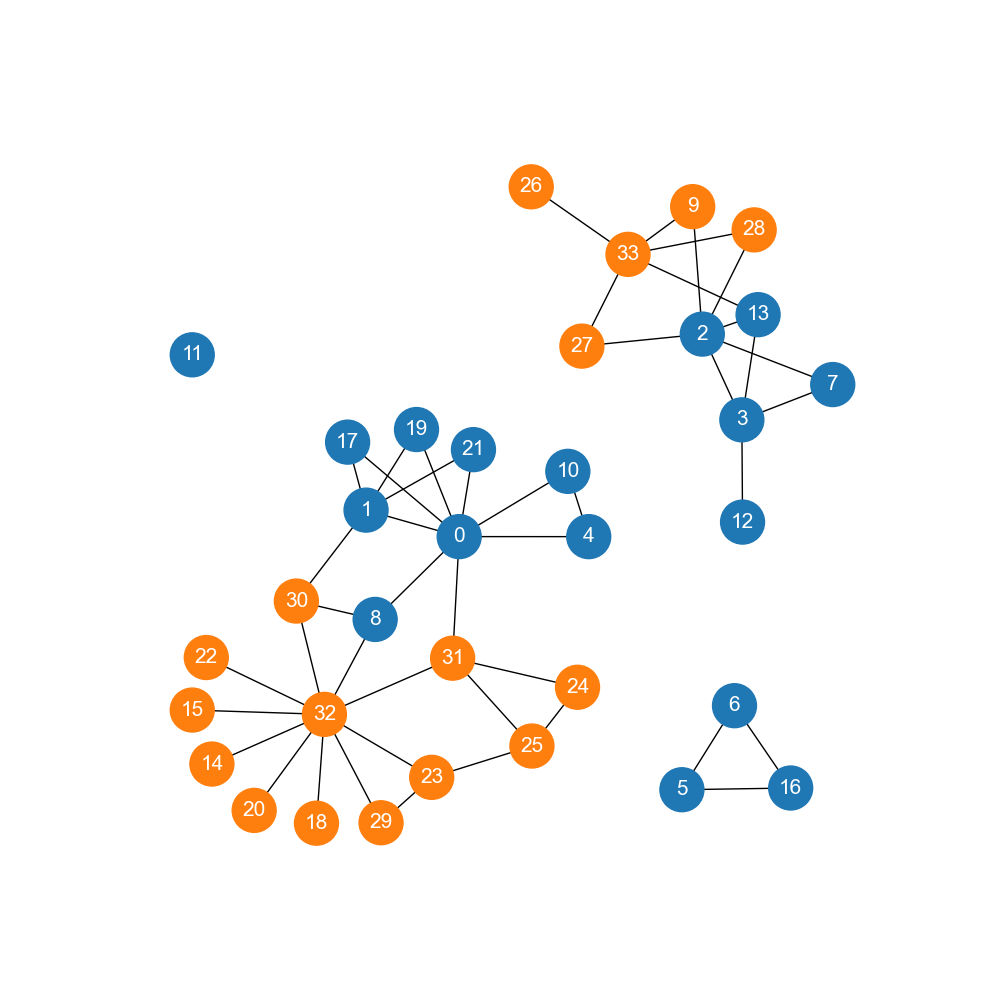
\includegraphics[width=.25\textwidth]{/files/src/.media/karate/grafo_corte_27_1.76.png}}\hfill
    \subfloat[av $\approx$ 1.83]{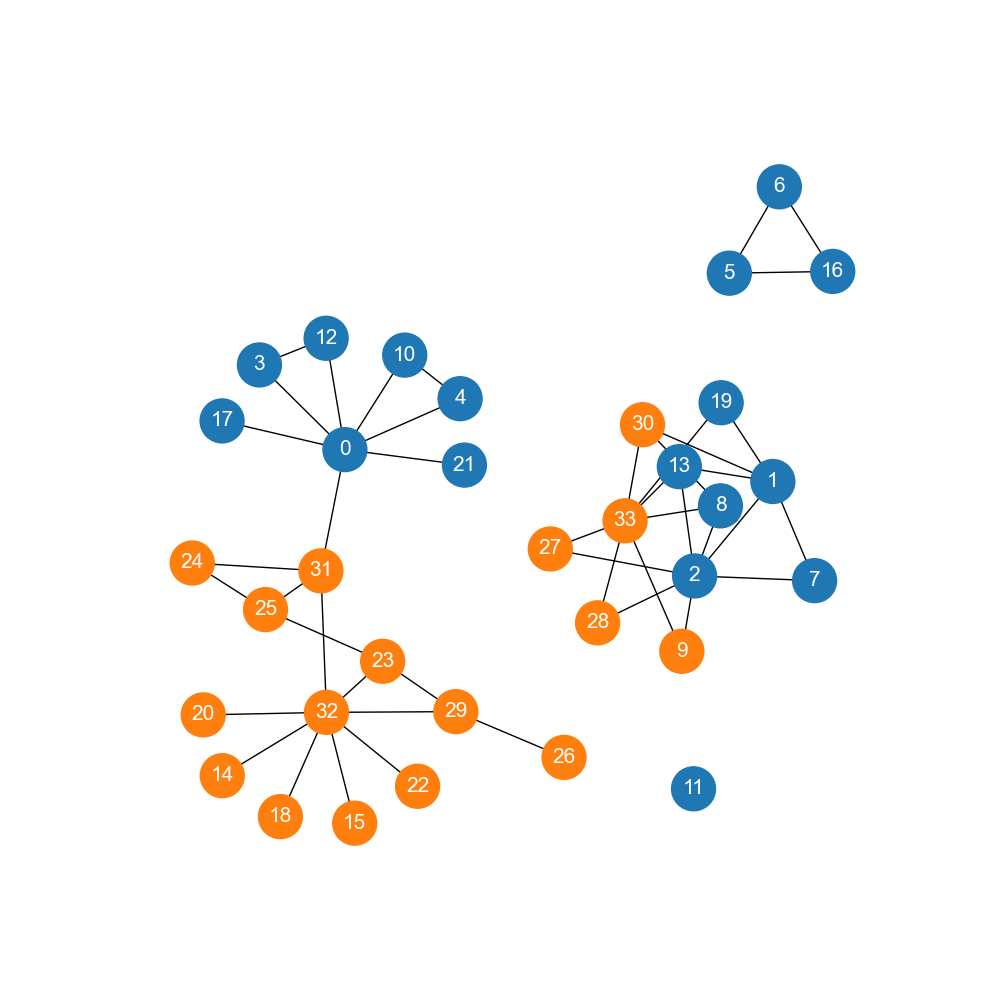
\includegraphics[width=.25\textwidth]{/files/src/.media/karate/grafo_corte_26_1.83.png}}\hfill
    \subfloat[av $\approx$ 1.96]{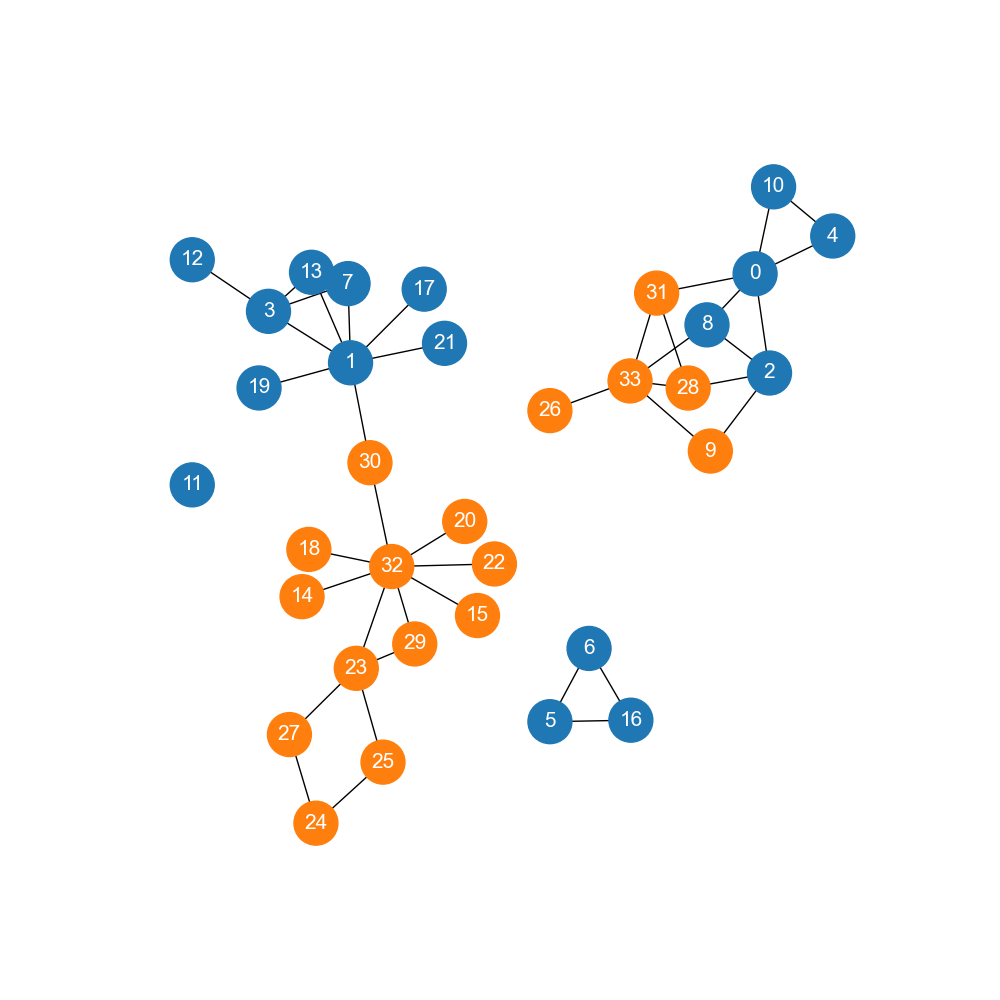
\includegraphics[width=.25\textwidth]{/files/src/.media/karate/grafo_corte_25_1.96.png}}\hfill
    \subfloat[av $\approx$ 2.00]{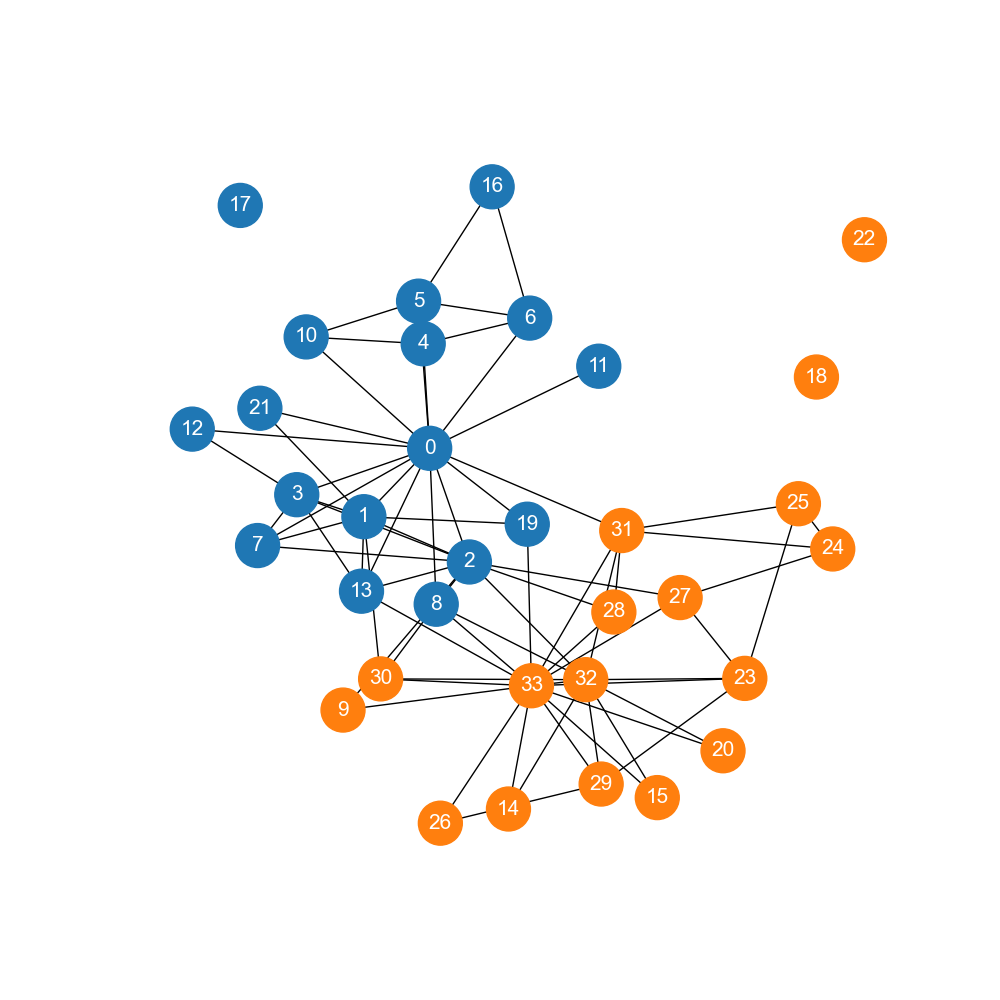
\includegraphics[width=.25\textwidth]{/files/src/.media/karate/grafo_corte_24_2.0.png}}\hfill
    \\[\smallskipamount]
    \subfloat[av $\approx$ 2.00]{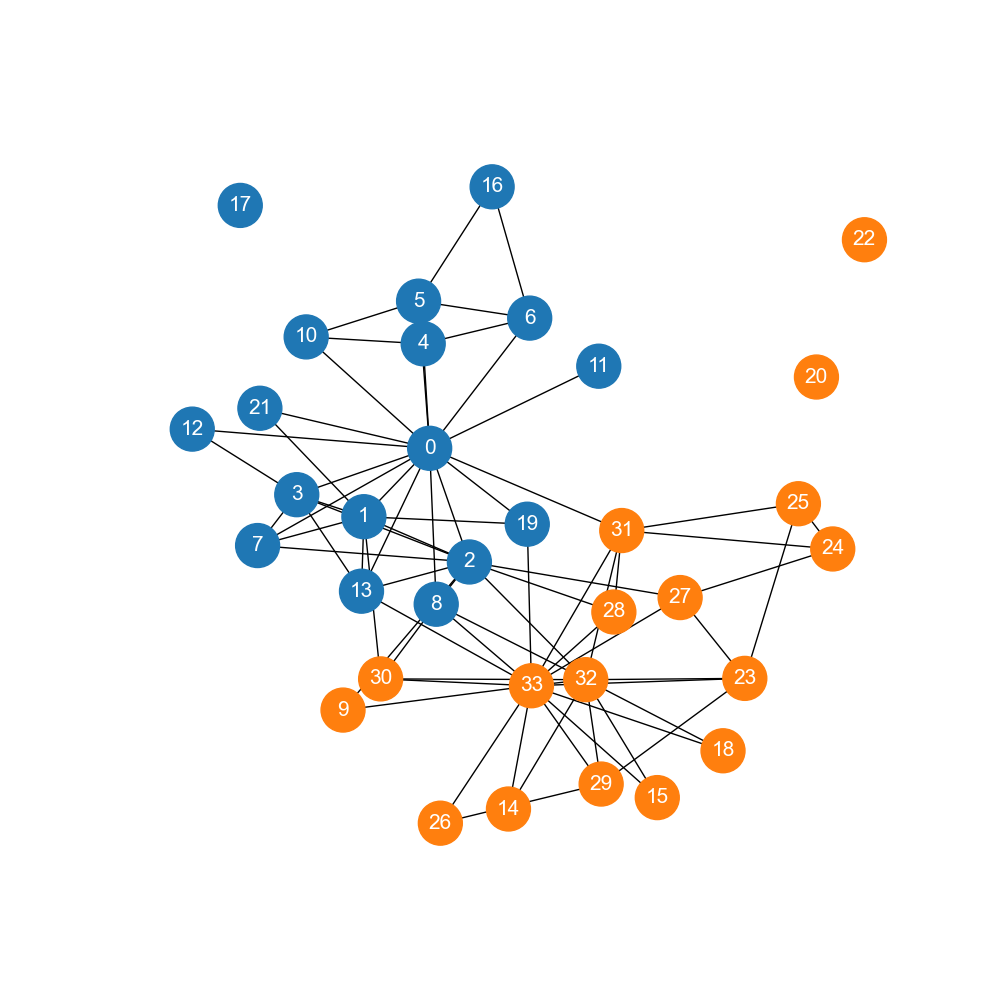
\includegraphics[width=.25\textwidth]{/files/src/.media/karate/grafo_corte_23_2.0.png}}\hfill
    \subfloat[av $\approx$ 2.00]{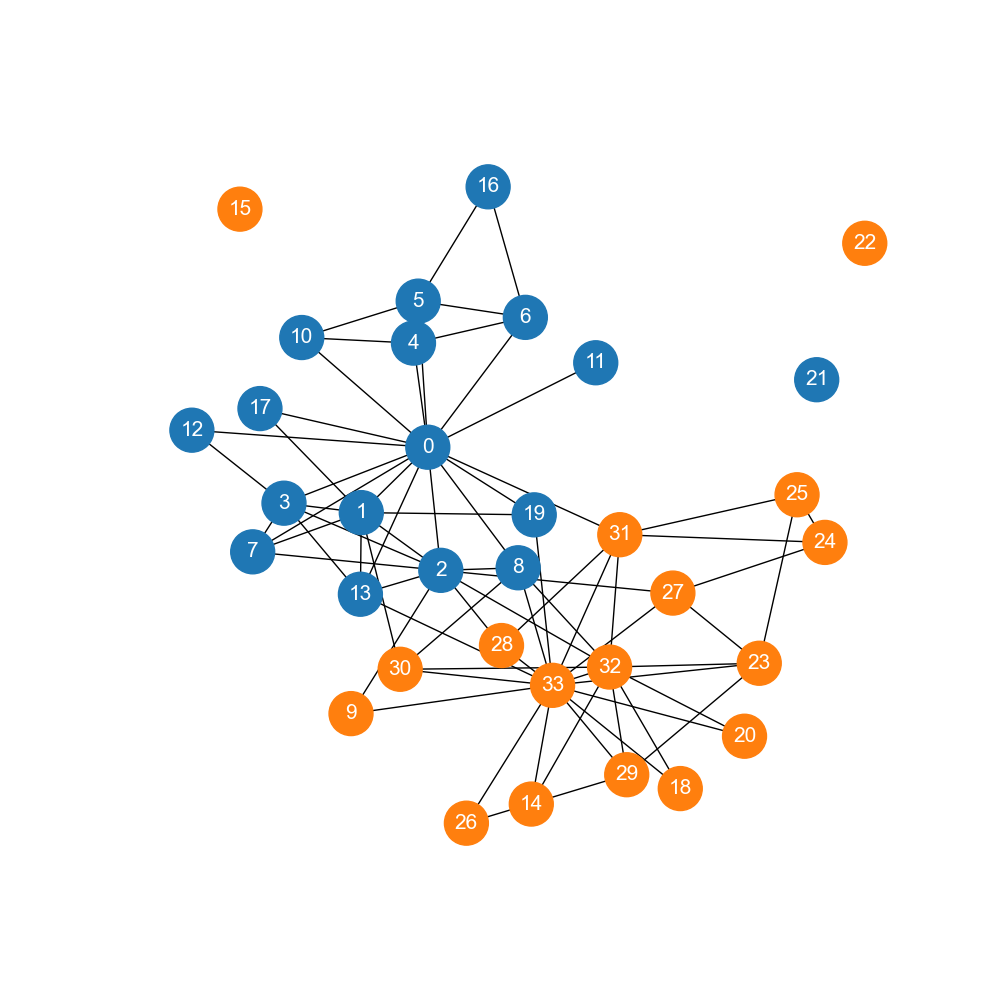
\includegraphics[width=.25\textwidth]{/files/src/.media/karate/grafo_corte_22_2.0.png}}\hfill
    \subfloat[av $\approx$ 2.00]{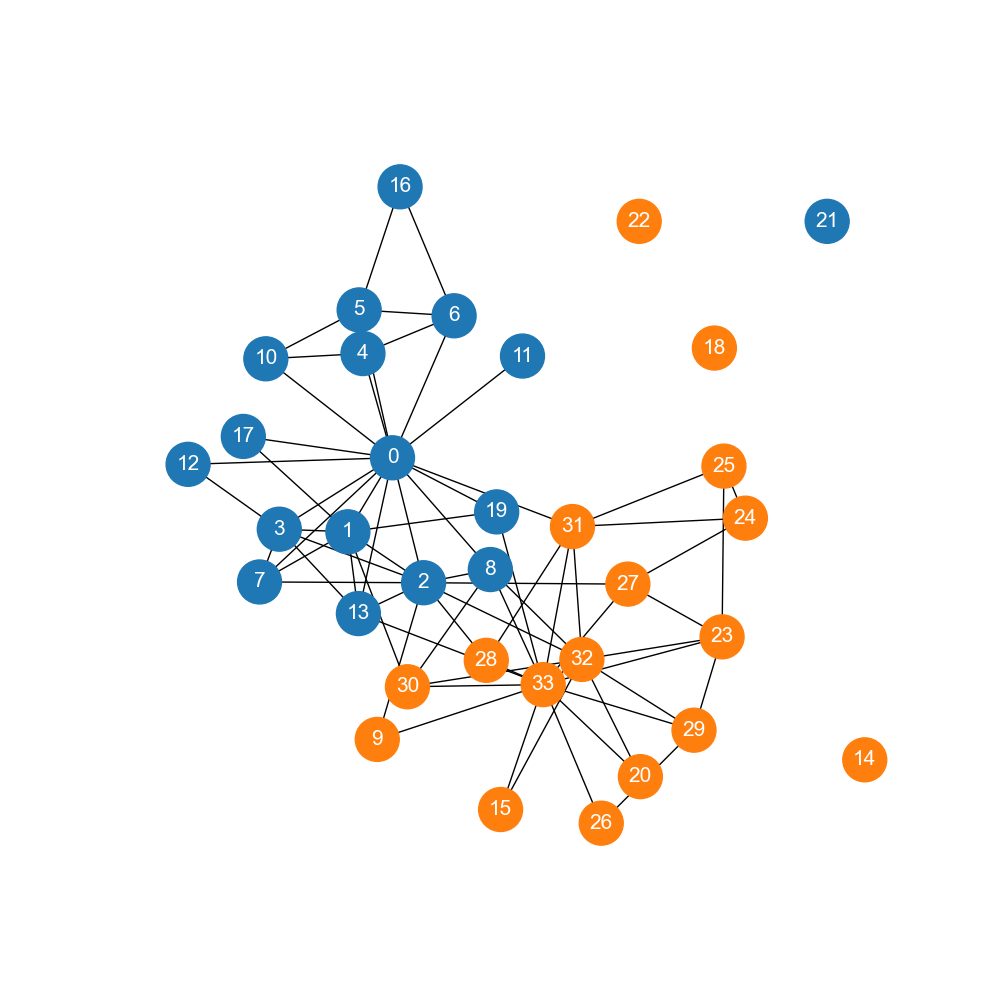
\includegraphics[width=.25\textwidth]{/files/src/.media/karate/grafo_corte_21_2.0.png}}\hfill
    \subfloat[av $\approx$ 2.00]{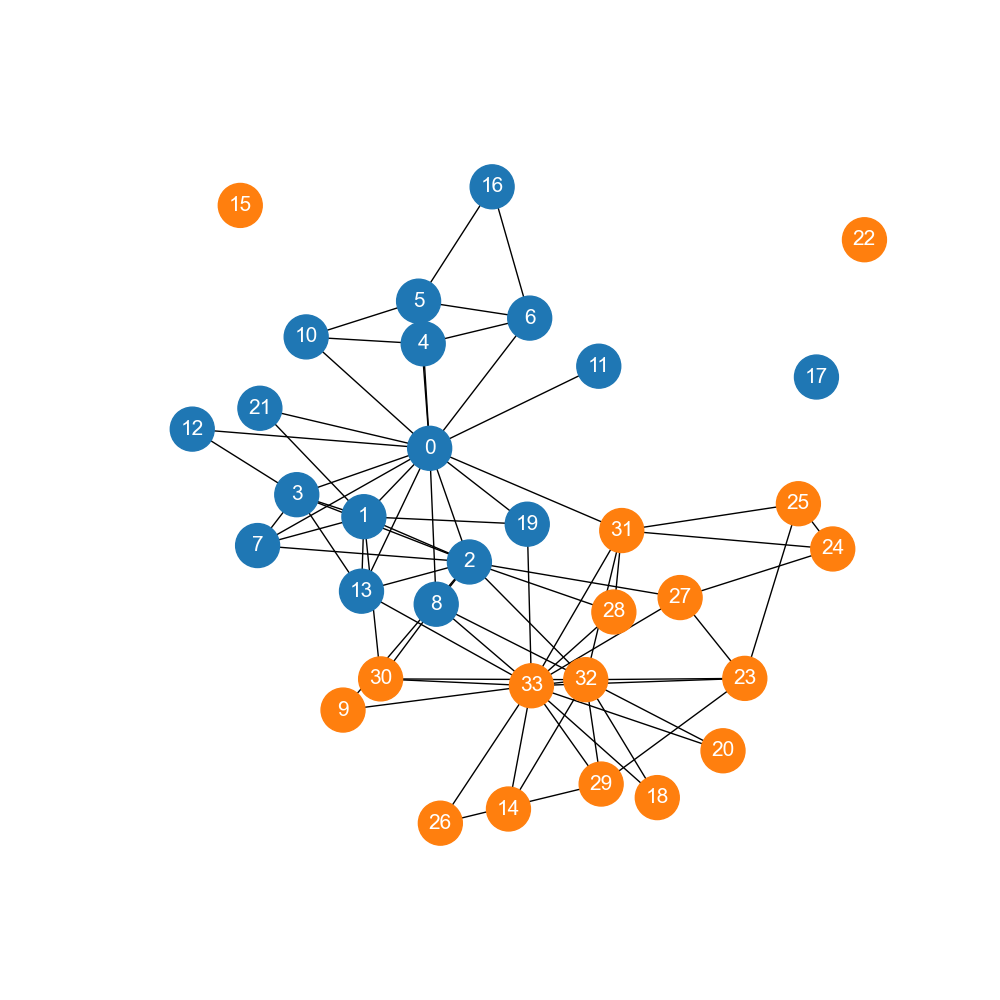
\includegraphics[width=.25\textwidth]{/files/src/.media/karate/grafo_corte_20_2.0.png}}\hfill
    \\[\smallskipamount]
    \subfloat[av $\approx$ 2.49]{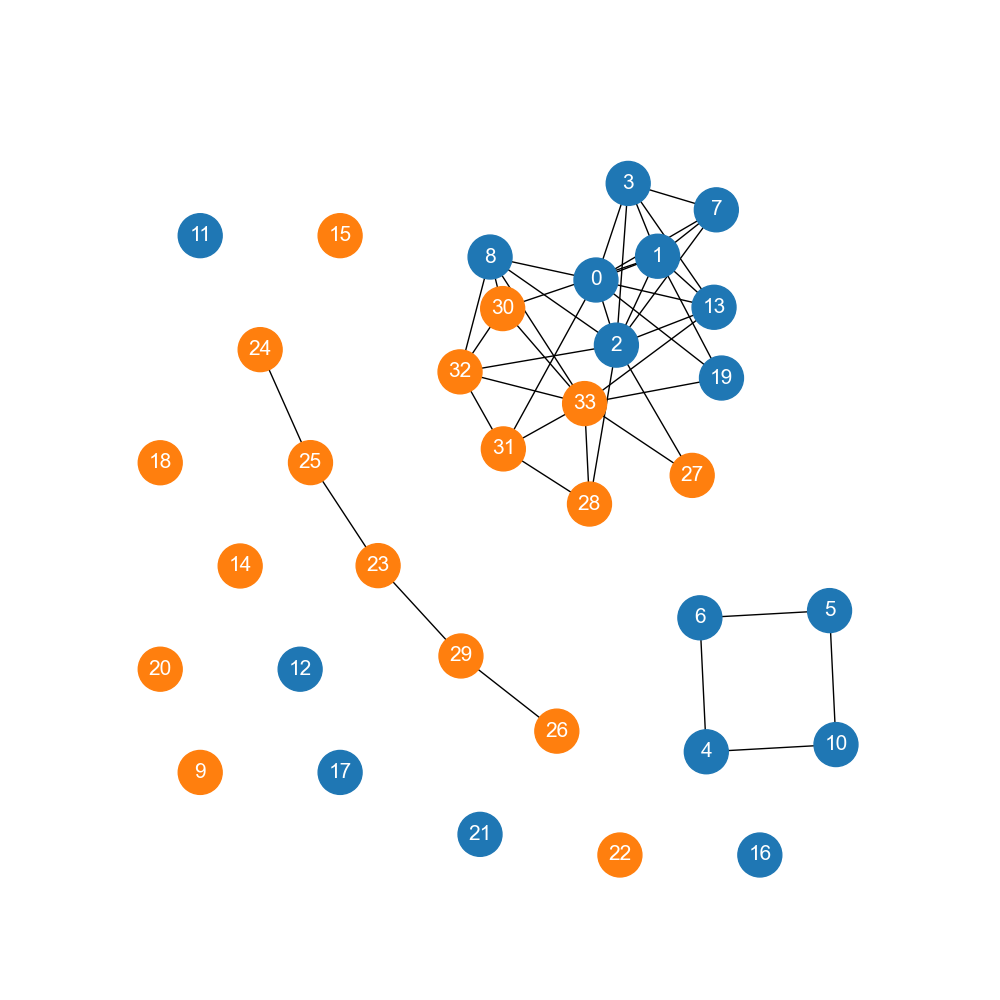
\includegraphics[width=.25\textwidth]{/files/src/.media/karate/grafo_corte_19_2.49.png}}\hfill
    \subfloat[av $\approx$ 2.75]{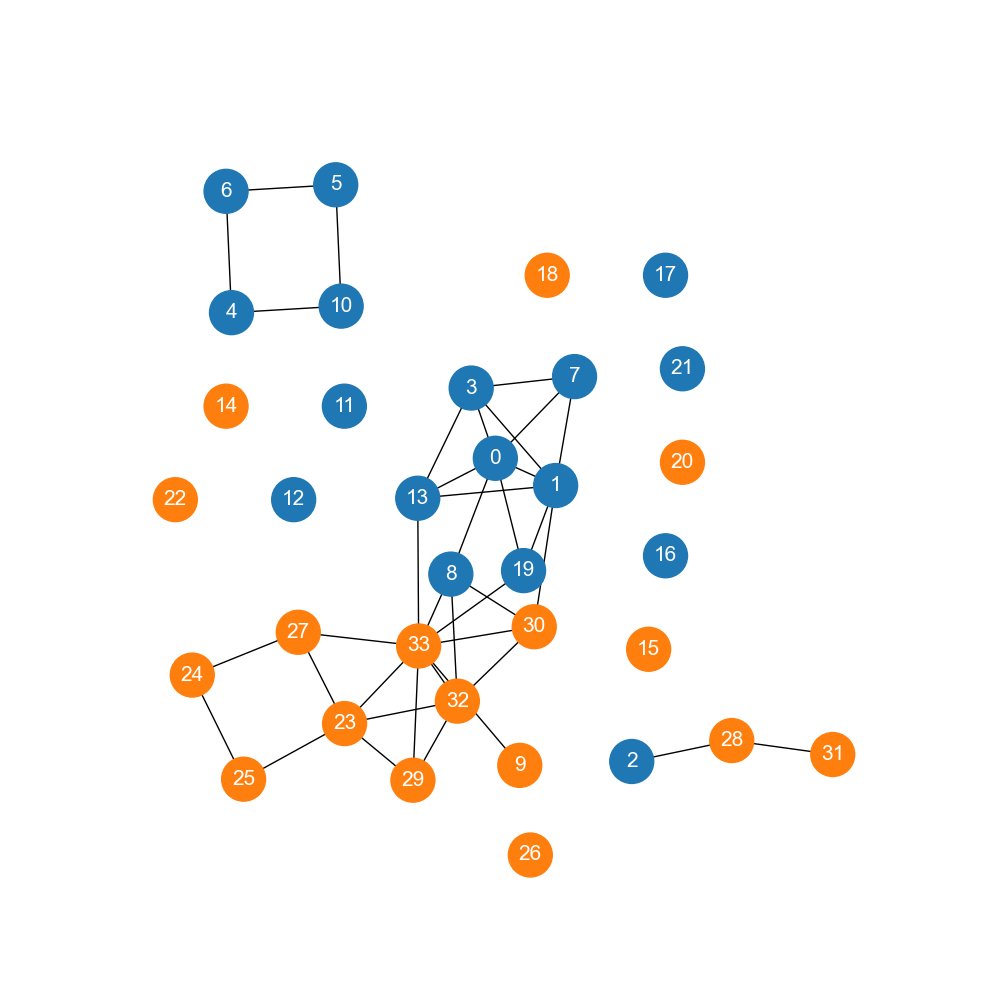
\includegraphics[width=.25\textwidth]{/files/src/.media/karate/grafo_corte_18_2.75.png}}\hfill
    \subfloat[av $\approx$ 3.01]{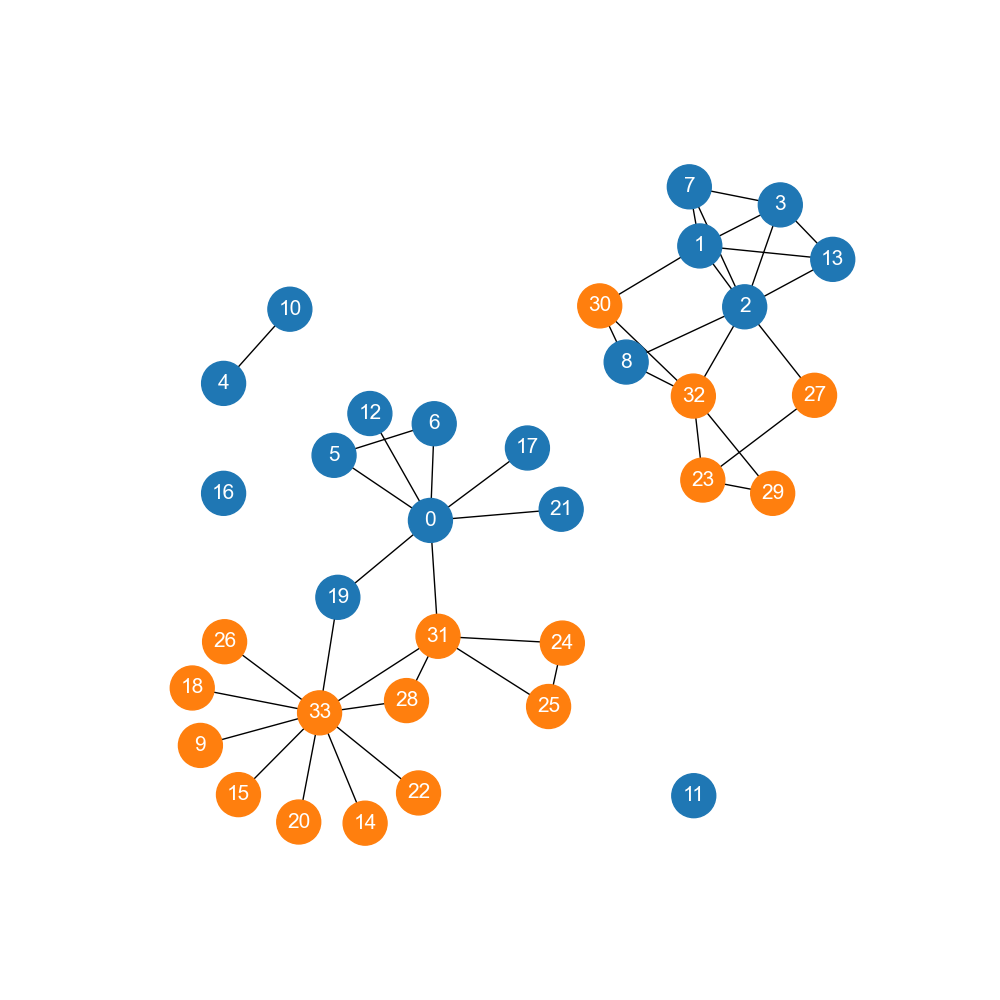
\includegraphics[width=.25\textwidth]{/files/src/.media/karate/grafo_corte_17_3.01.png}}\hfill
    \subfloat[av $\approx$ 3.24]{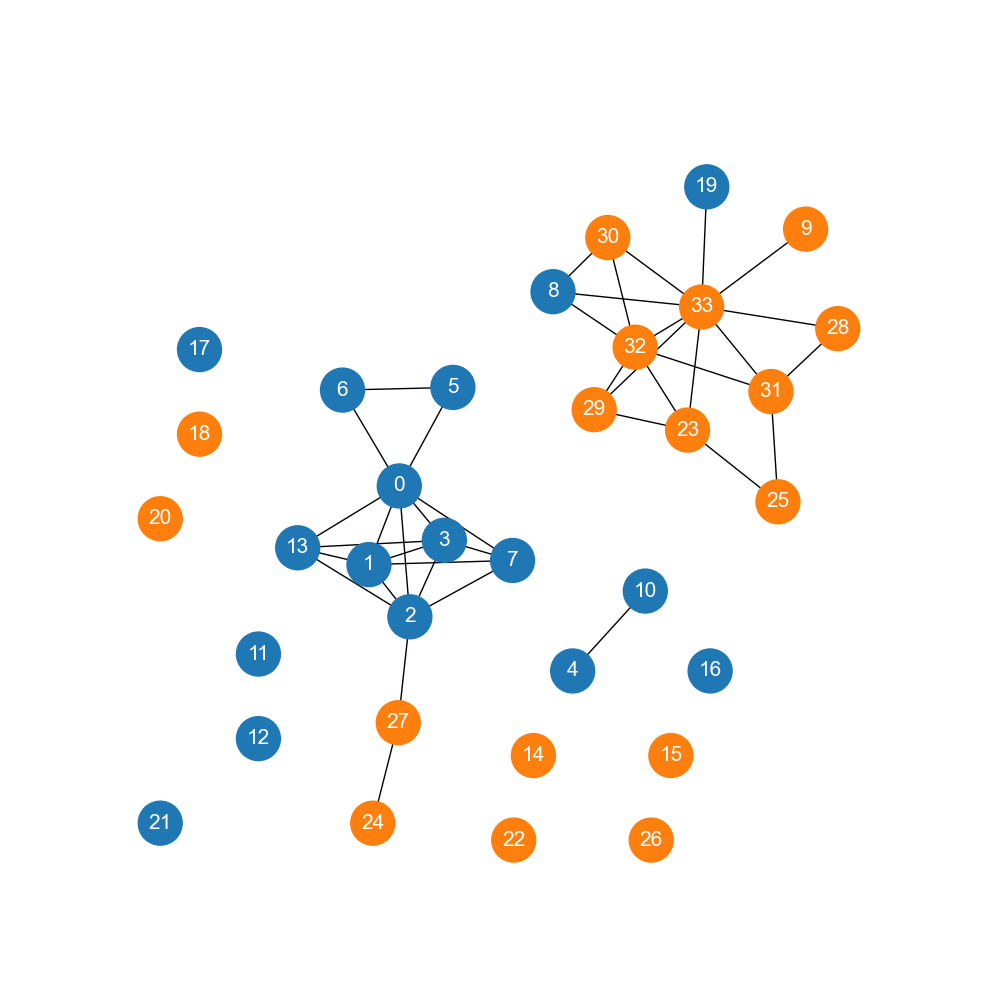
\includegraphics[width=.25\textwidth]{/files/src/.media/karate/grafo_corte_16_3.24.png}}\hfill
\end{figure}

\begin{figure}[!htbp]
    \ContinuedFloat
    \centering
    \subfloat[av $\approx$ 3.38]{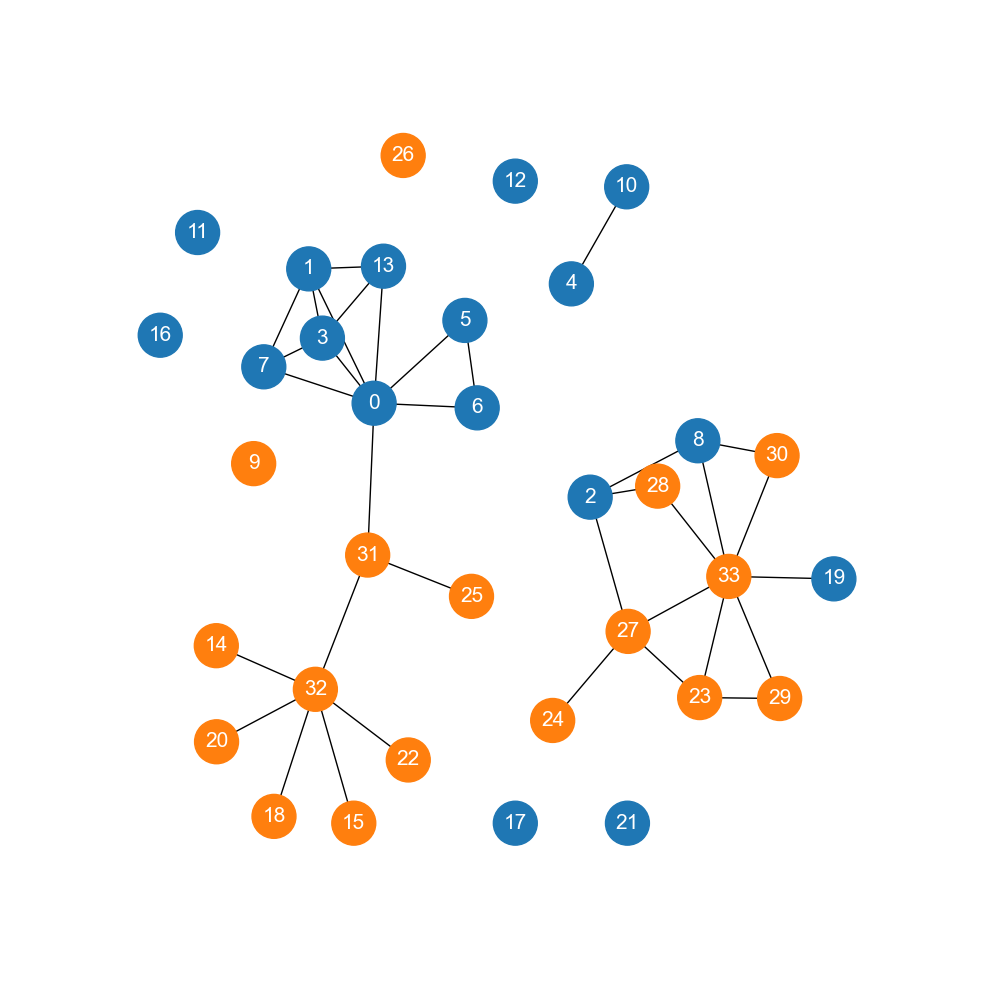
\includegraphics[width=.25\textwidth]{/files/src/.media/karate/grafo_corte_15_3.38.png}}\hfill
    \subfloat[av $\approx$ 3.38]{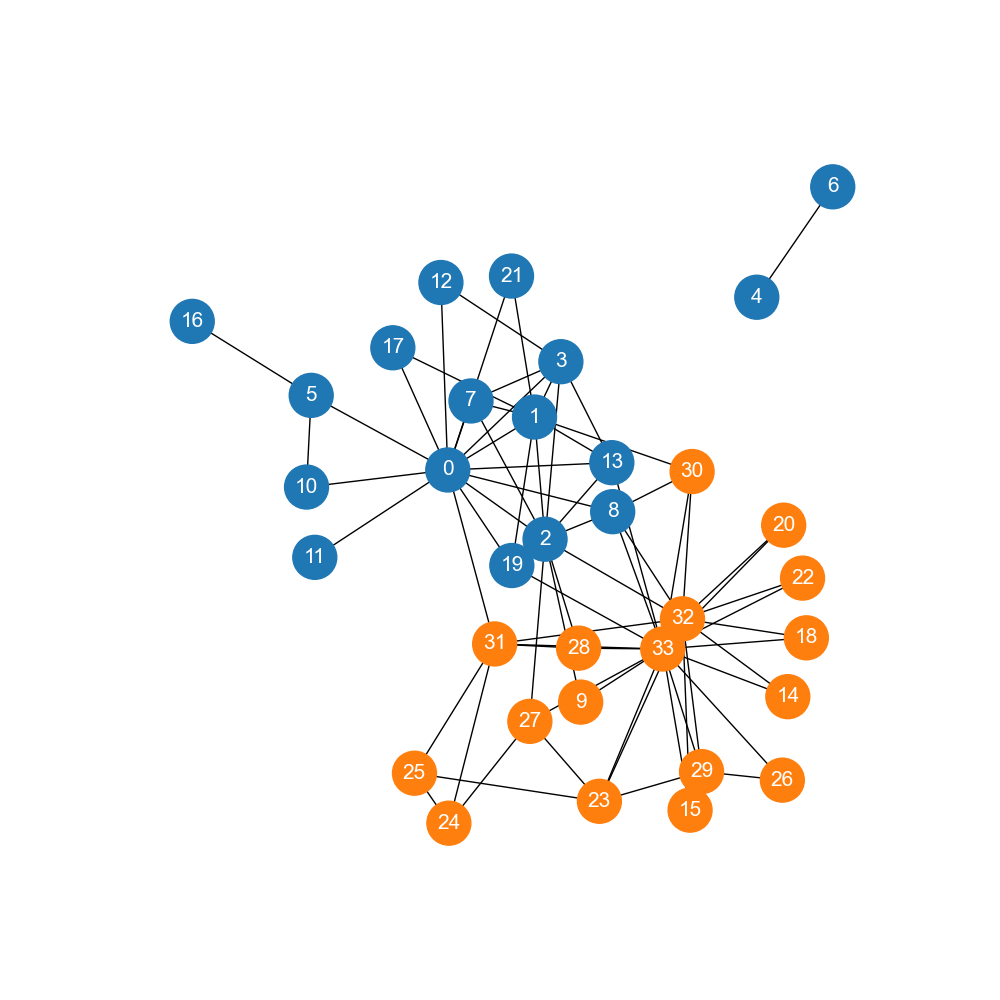
\includegraphics[width=.25\textwidth]{/files/src/.media/karate/grafo_corte_14_3.38.png}}\hfill
    \subfloat[av $\approx$ 3.47]{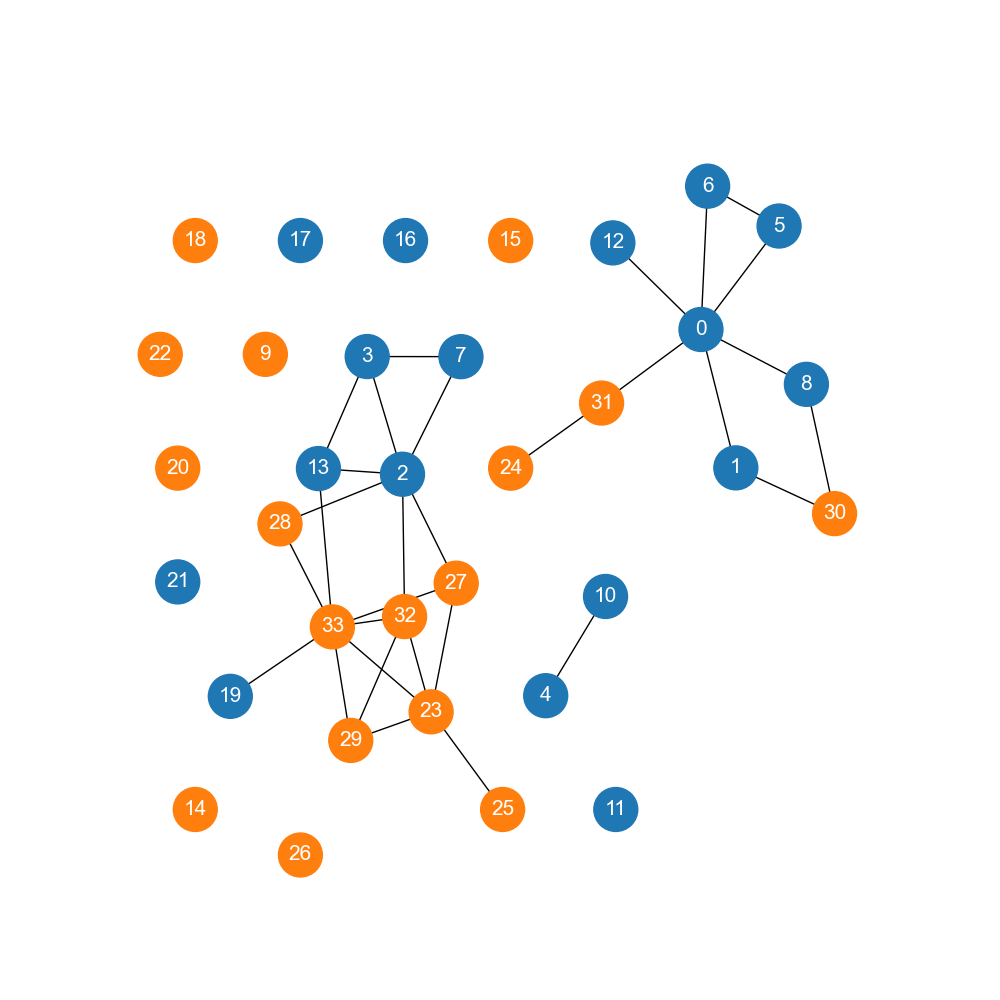
\includegraphics[width=.25\textwidth]{/files/src/.media/karate/grafo_corte_13_3.47.png}}\hfill
    \subfloat[av $\approx$ 4.28]{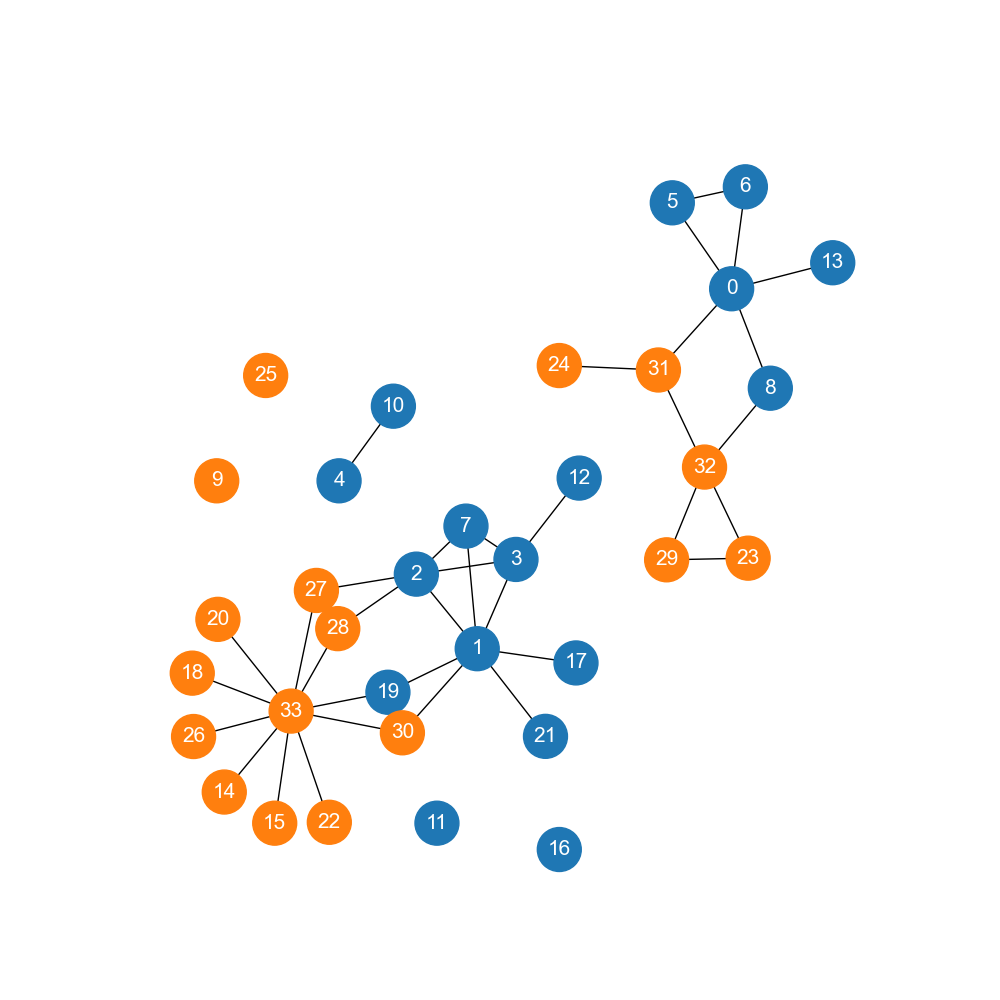
\includegraphics[width=.25\textwidth]{/files/src/.media/karate/grafo_corte_12_4.28.png}}\hfill
    \\[\smallskipamount]
    \subfloat[av $\approx$ 4.48]{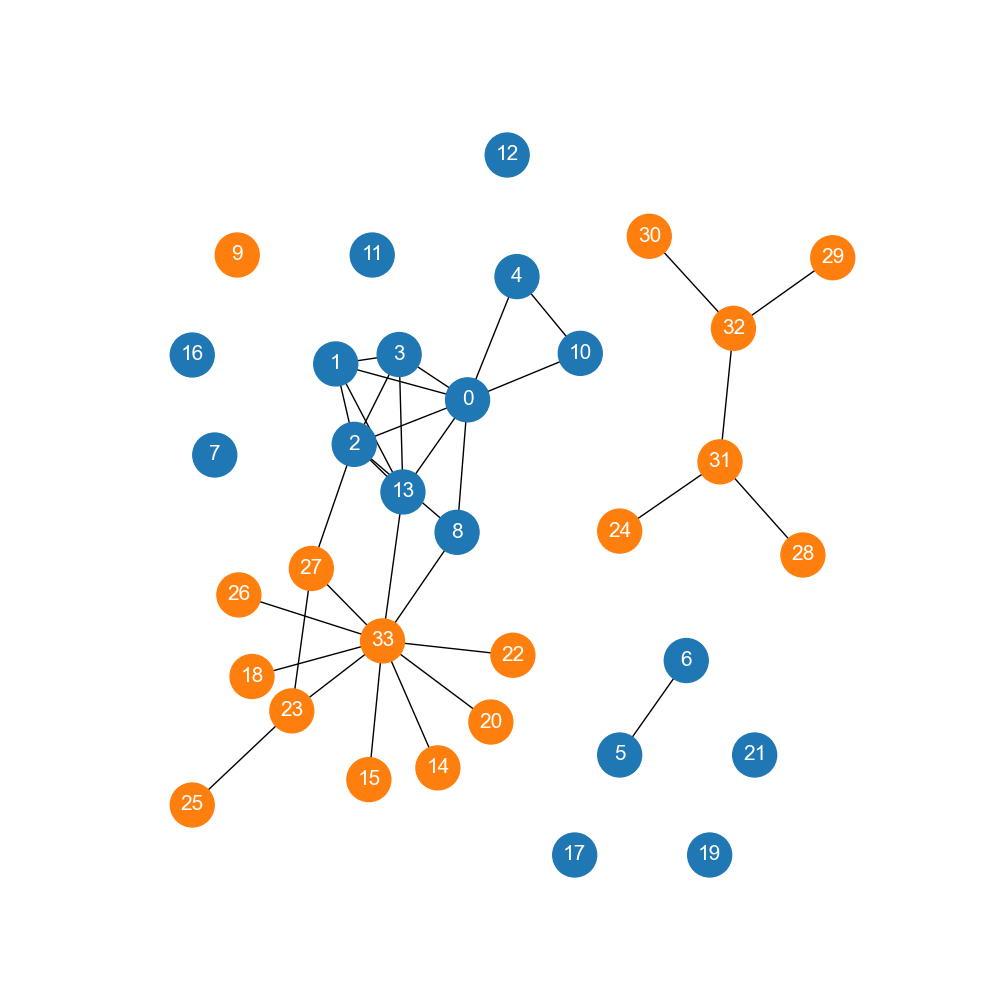
\includegraphics[width=.25\textwidth]{/files/src/.media/karate/grafo_corte_11_4.48.png}}\hfill
    \subfloat[av $\approx$ 4.58]{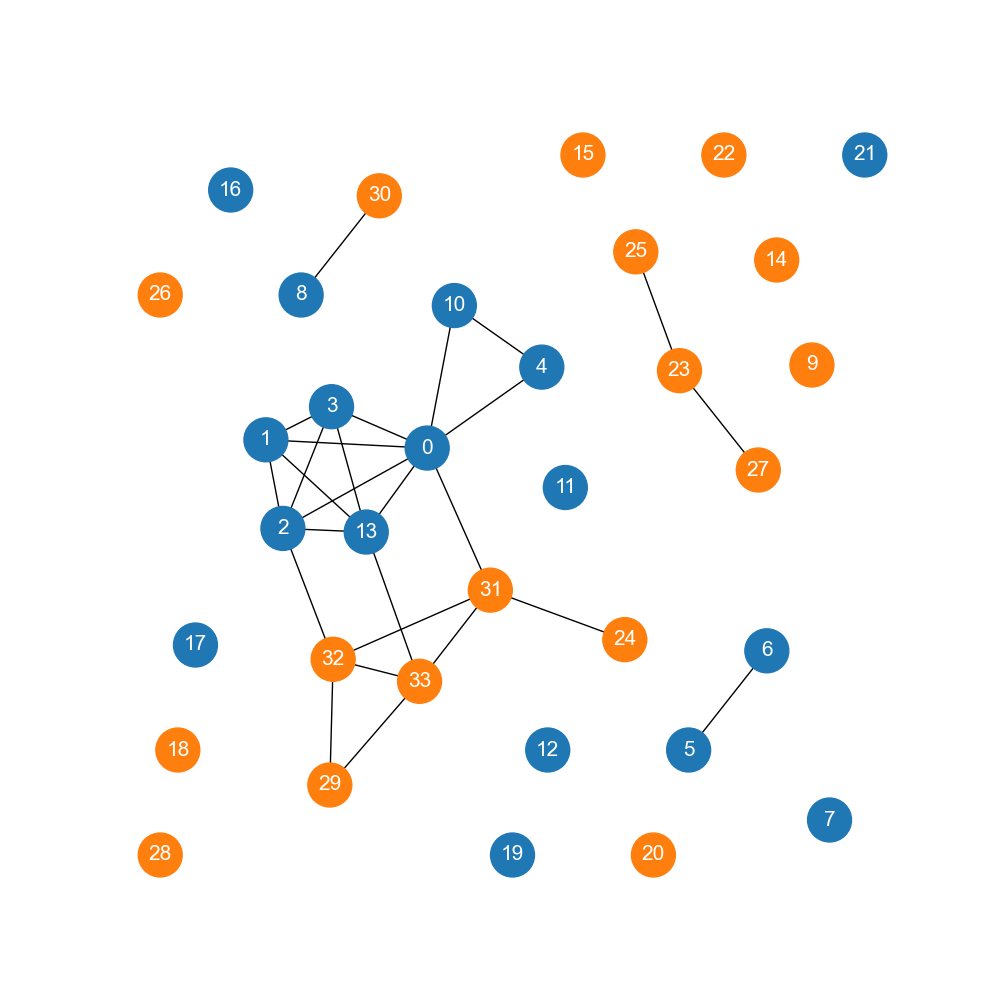
\includegraphics[width=.25\textwidth]{/files/src/.media/karate/grafo_corte_10_4.58.png}}\hfill
    \subfloat[av $\approx$ 5.38]{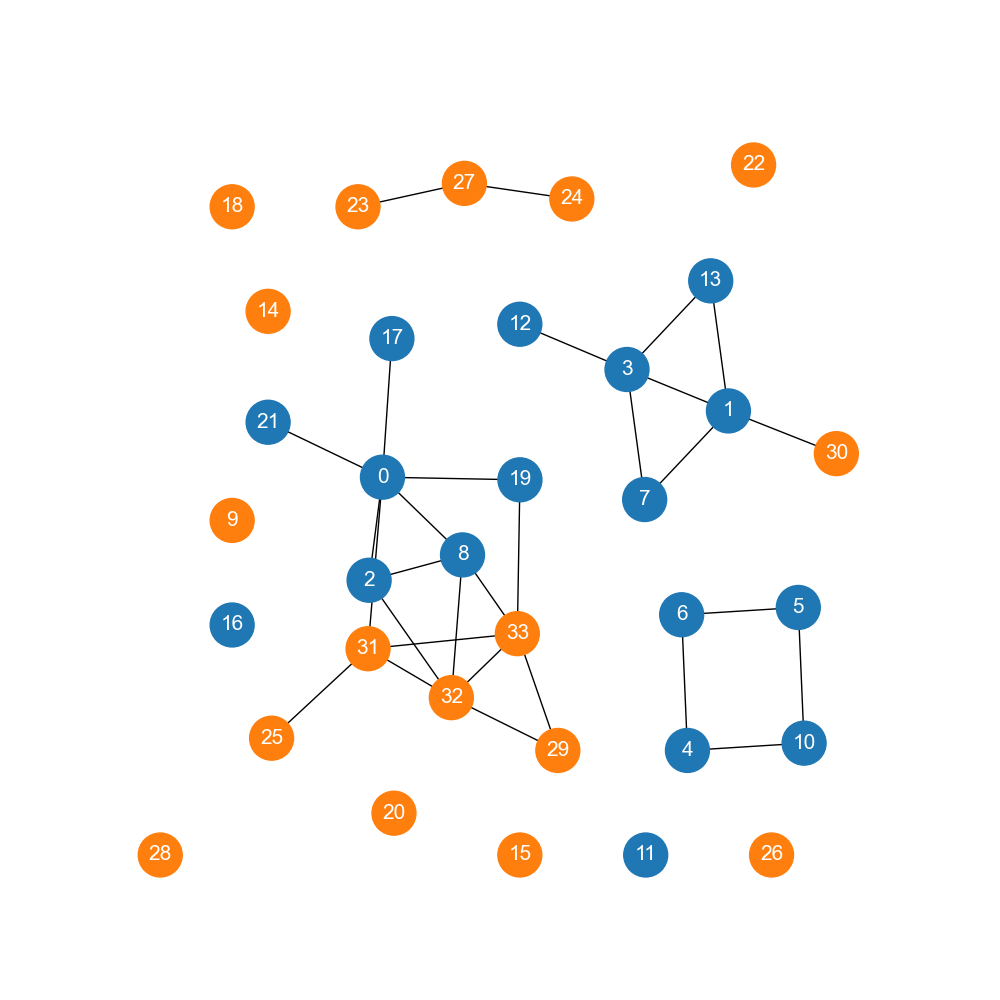
\includegraphics[width=.25\textwidth]{/files/src/.media/karate/grafo_corte_9_5.38.png}}\hfill
    \subfloat[av $\approx$ 5.62]{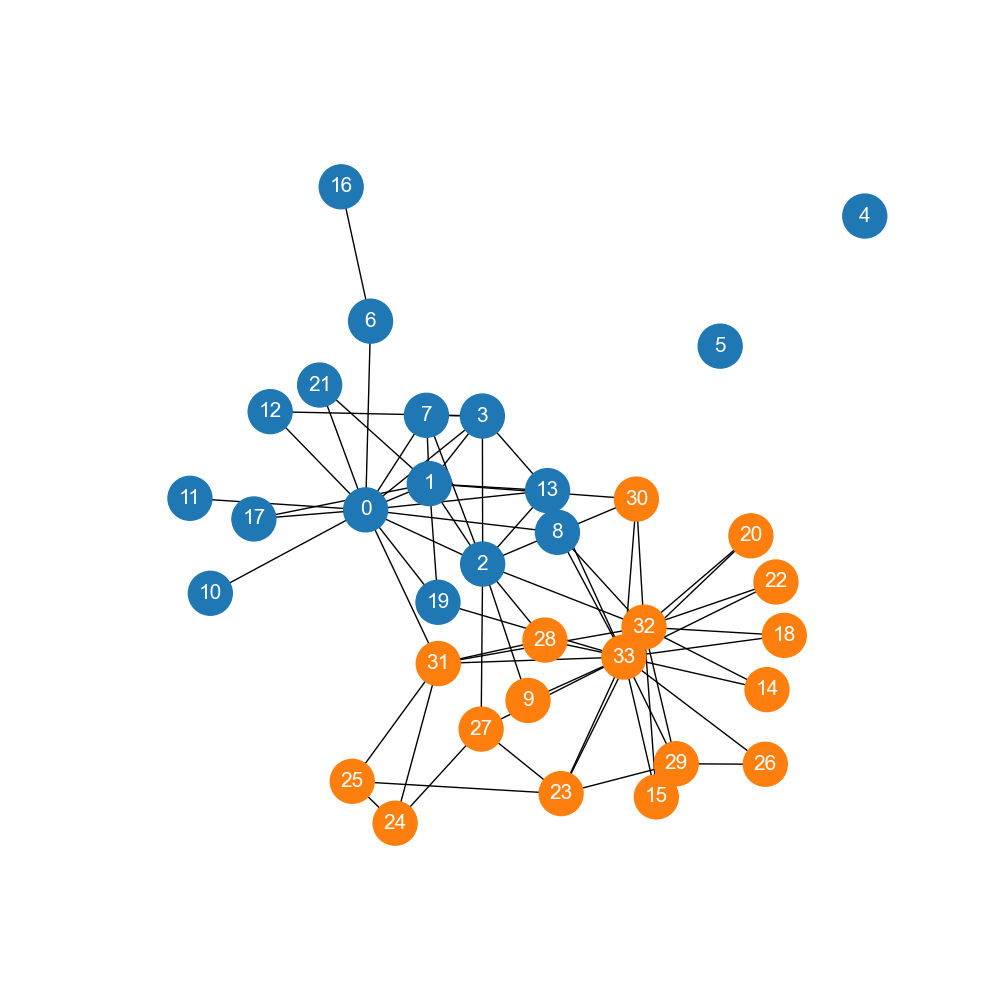
\includegraphics[width=.25\textwidth]{/files/src/.media/karate/grafo_corte_8_5.62.png}}\hfill
    \\[\smallskipamount]
    \subfloat[av $\approx$ 6.33]{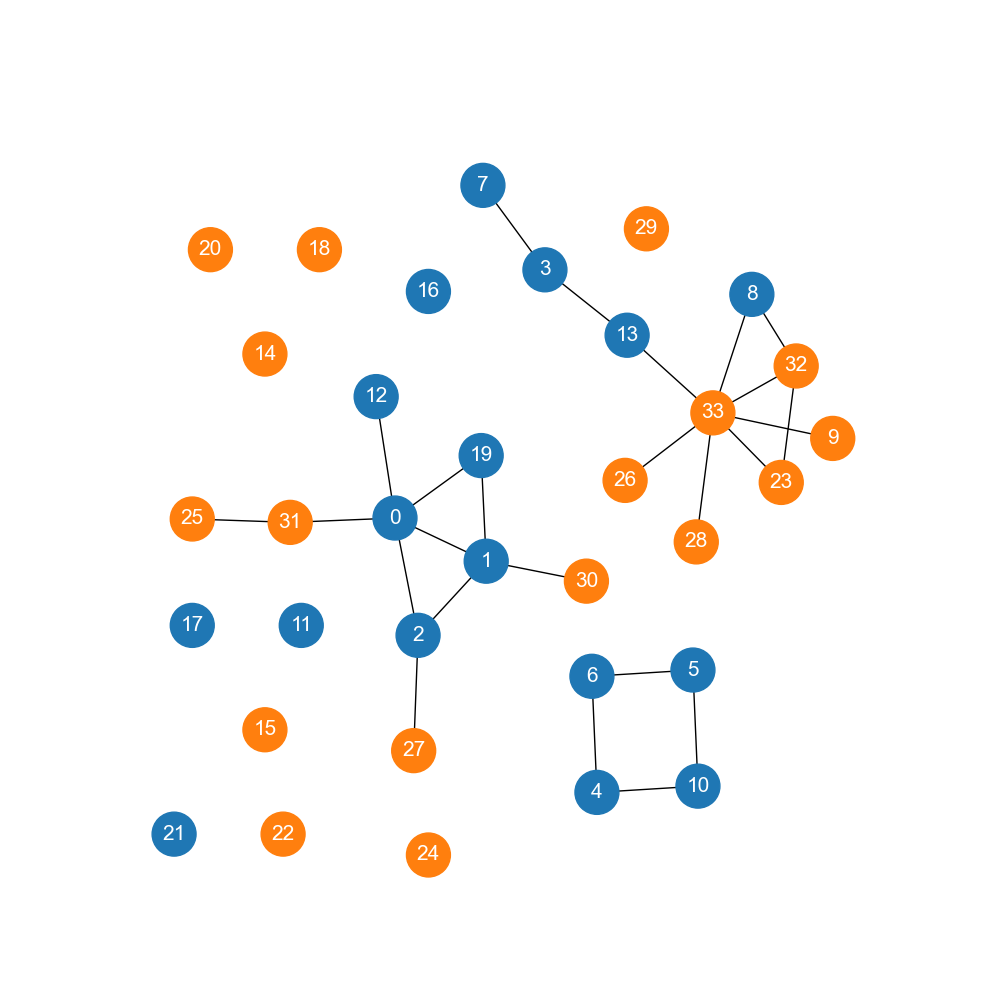
\includegraphics[width=.25\textwidth]{/files/src/.media/karate/grafo_corte_7_6.33.png}}\hfill
    \subfloat[av $\approx$ 6.52]{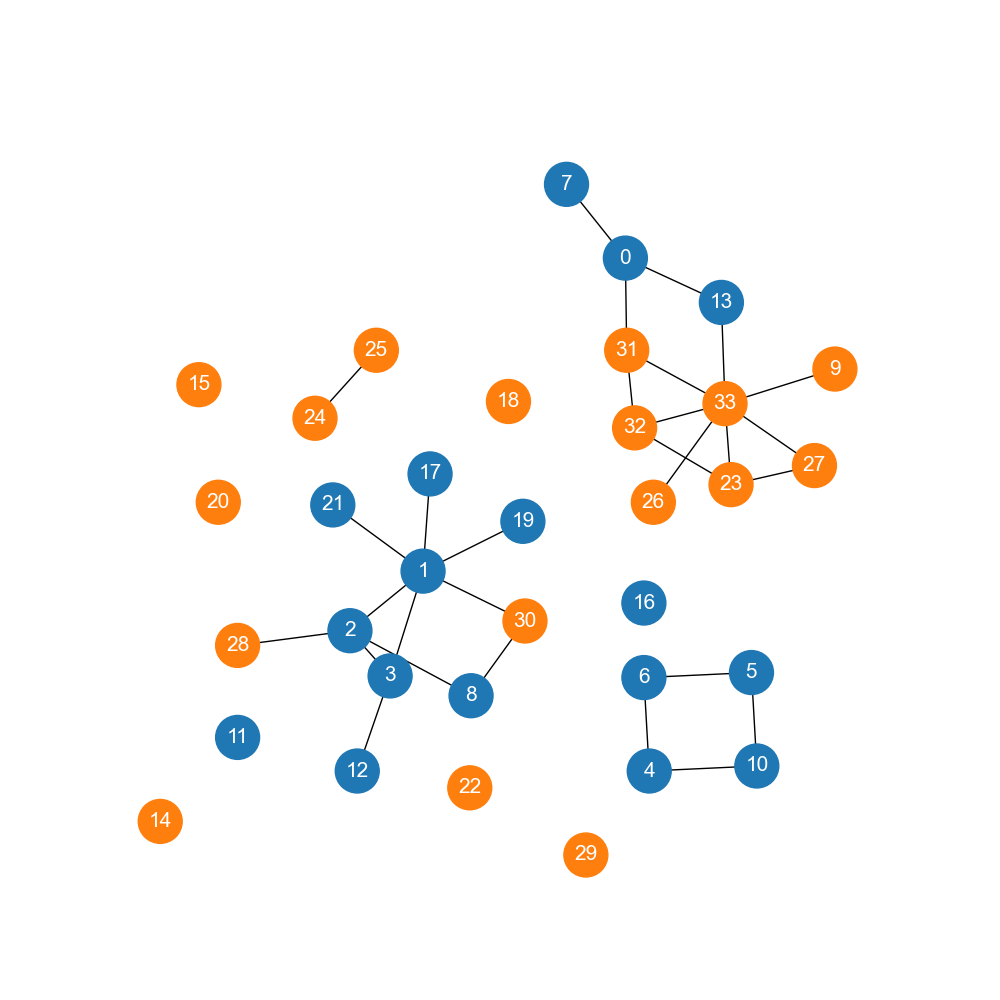
\includegraphics[width=.25\textwidth]{/files/src/.media/karate/grafo_corte_6_6.52.png}}\hfill
    \subfloat[av $\approx$ 7.0]{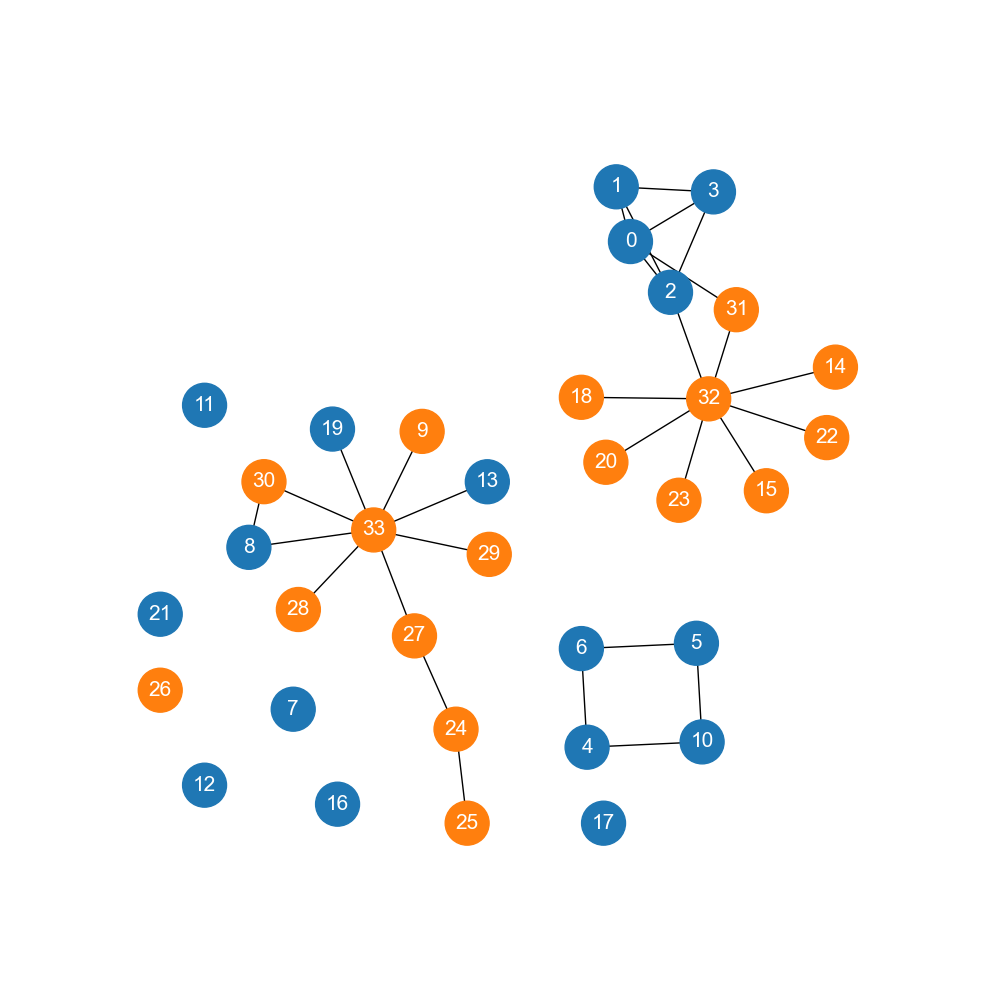
\includegraphics[width=.25\textwidth]{/files/src/.media/karate/grafo_corte_5_7.0.png}}\hfill
    \subfloat[av $\approx$ 9.78]{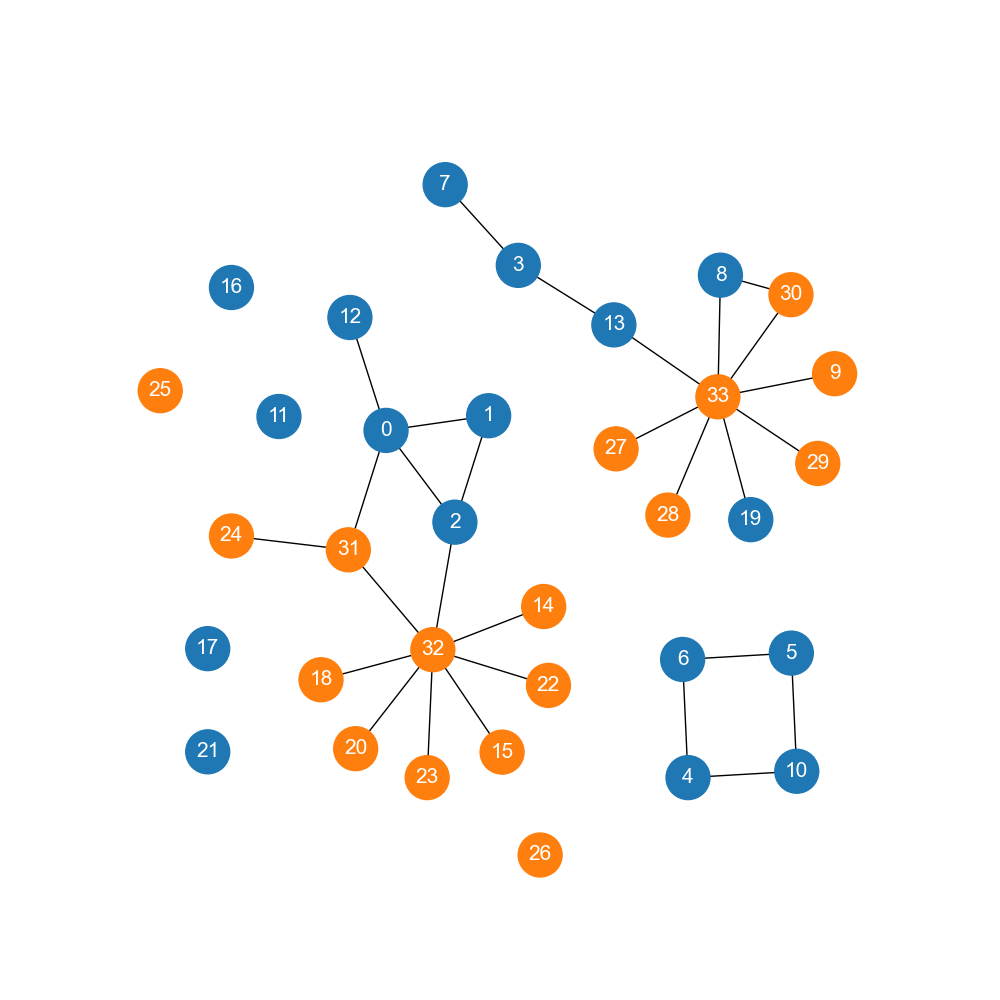
\includegraphics[width=.25\textwidth]{/files/src/.media/karate/grafo_corte_4_9.78.png}}\hfill
    \\[\smallskipamount]
    \subfloat[av $\approx$ 10.92]{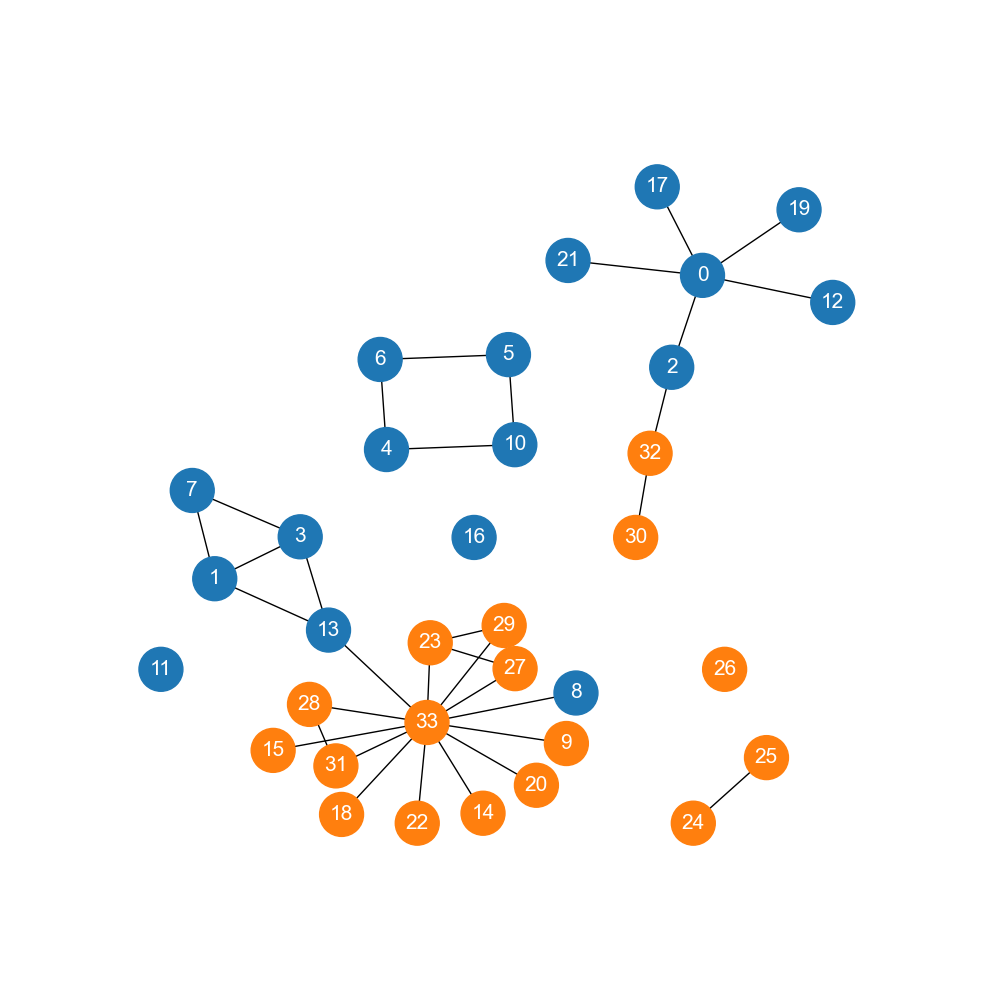
\includegraphics[width=.25\textwidth]{/files/src/.media/karate/grafo_corte_3_10.92.png}}\hfill
    \subfloat[av $\approx$ 13.31]{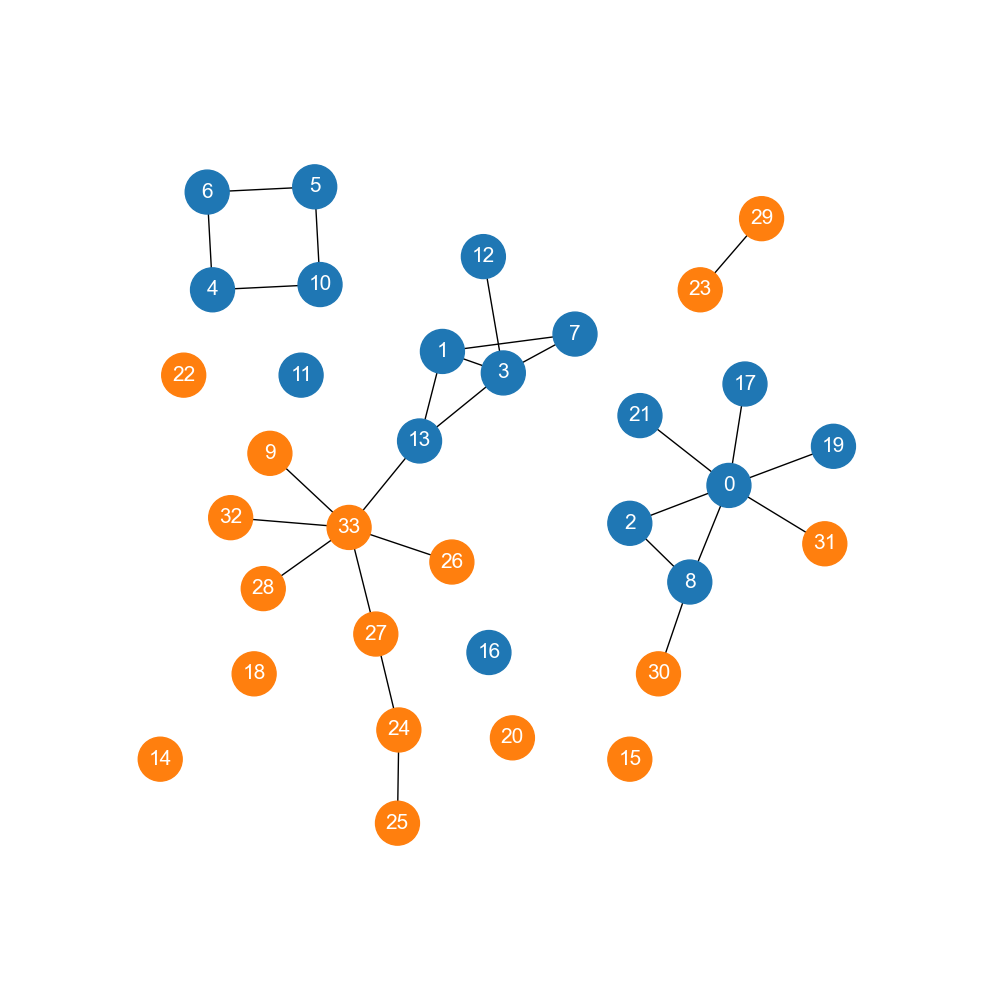
\includegraphics[width=.25\textwidth]{/files/src/.media/karate/grafo_corte_2_13.31.png}}\hfill
    \subfloat[av $\approx$ 17.06]{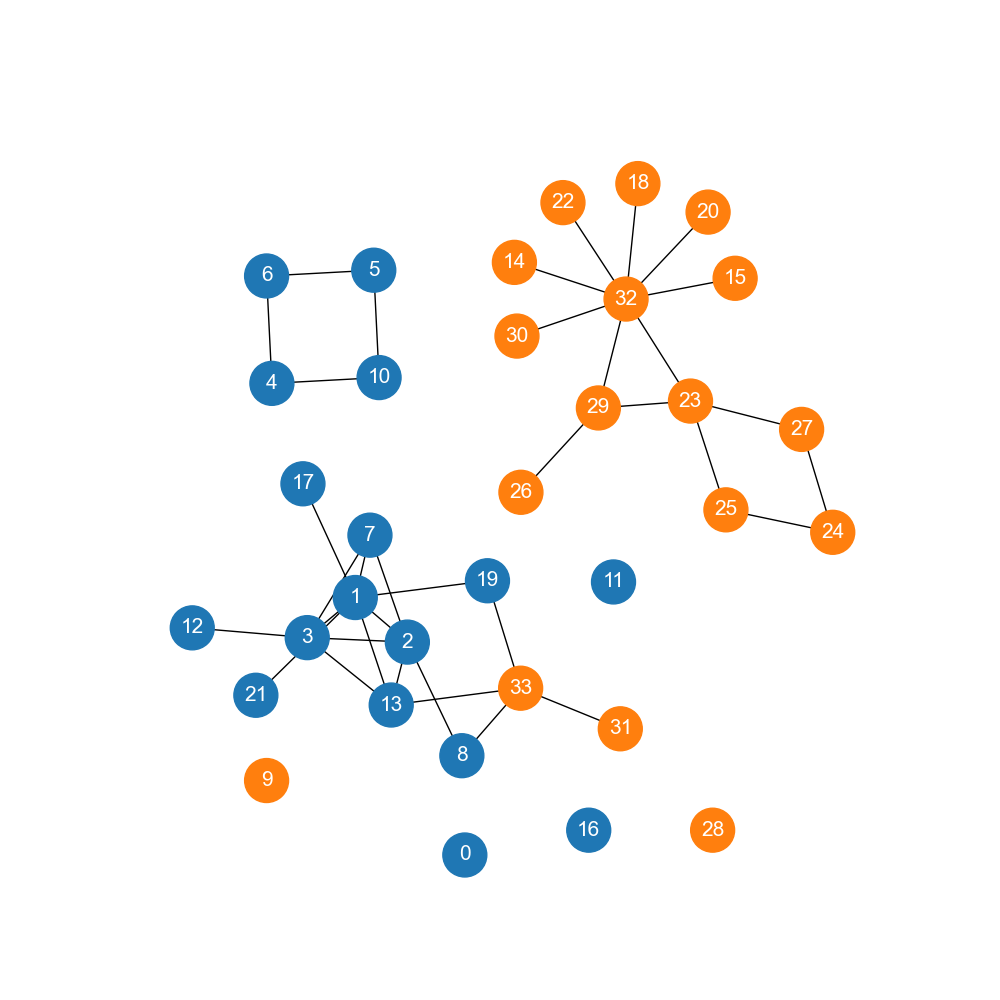
\includegraphics[width=.25\textwidth]{/files/src/.media/karate/grafo_corte_1_17.06.png}}\hfill
    \subfloat[av $\approx$ 18.14]{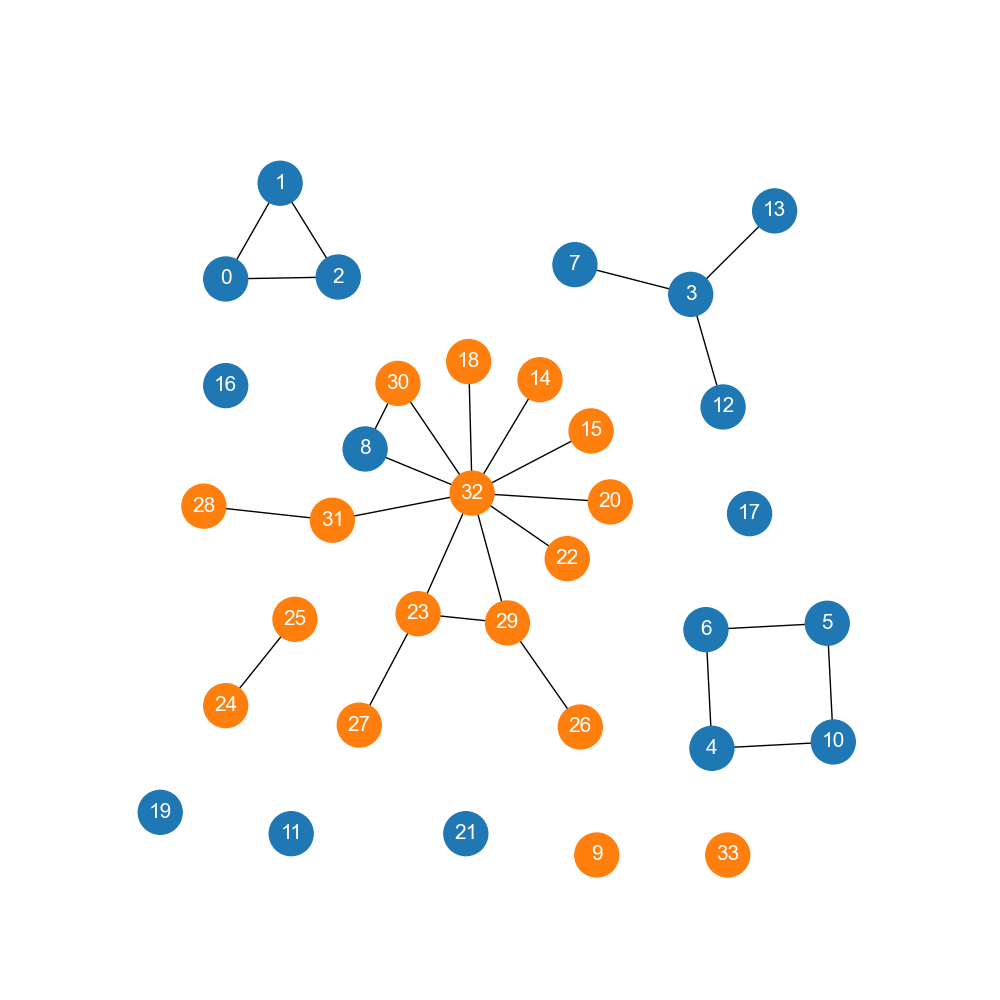
\includegraphics[width=.25\textwidth]{/files/src/.media/karate/grafo_corte_0_18.14.png}}\hfill
    \\[\smallskipamount]
    \caption{Todos los cortes posibles ---salvo el de Fiedler y el nulo---, correspondientes a los autovectores asociados a la matriz laplaciana de la red del \textit{Club de Karate}. Cada uno se designa por medio de su autovalor.} \label{grafos_av}
\end{figure}

\newpage

% facebook
\section{Análisis: Red `Ego'}
% === CONTEXTO === %

\vspace{2em}
\subsection{Contexto} 

En el análisis de redes sociales, una \textit{ego-network} \cite{Leskovec} es una red compuesta por las amistades que existen entre los amigos de un individuo, el `ego'. Estas redes son centrales en aplicaciones como Facebook, Google+ o Twitter. 

\vspace{1em}
En particular, dada una red de estas características, resulta de interés poder identificar los círculos sociales ---conjuntos, disjuntos y anidados--- a los que pertenece un usuario. Leskovec \cite{Leskovec} propone un método de aprendizaje no supervisado para lograr inferirlos, que se nutre de la siguiente información: un grafo \textbf{E} (la red) ---donde se espera que exista una correlación fuerte entre un círculo y la densidad de conexiones entre los nodos que lo componen--- y un conjunto de atributos \textbf{C} para cada nodo ---donde se espera que exista una correlación entre un círculo y la similaridad de los atributos de los nodos que lo componen---.

\vspace{1em}
\begin{figure}[!htbp]
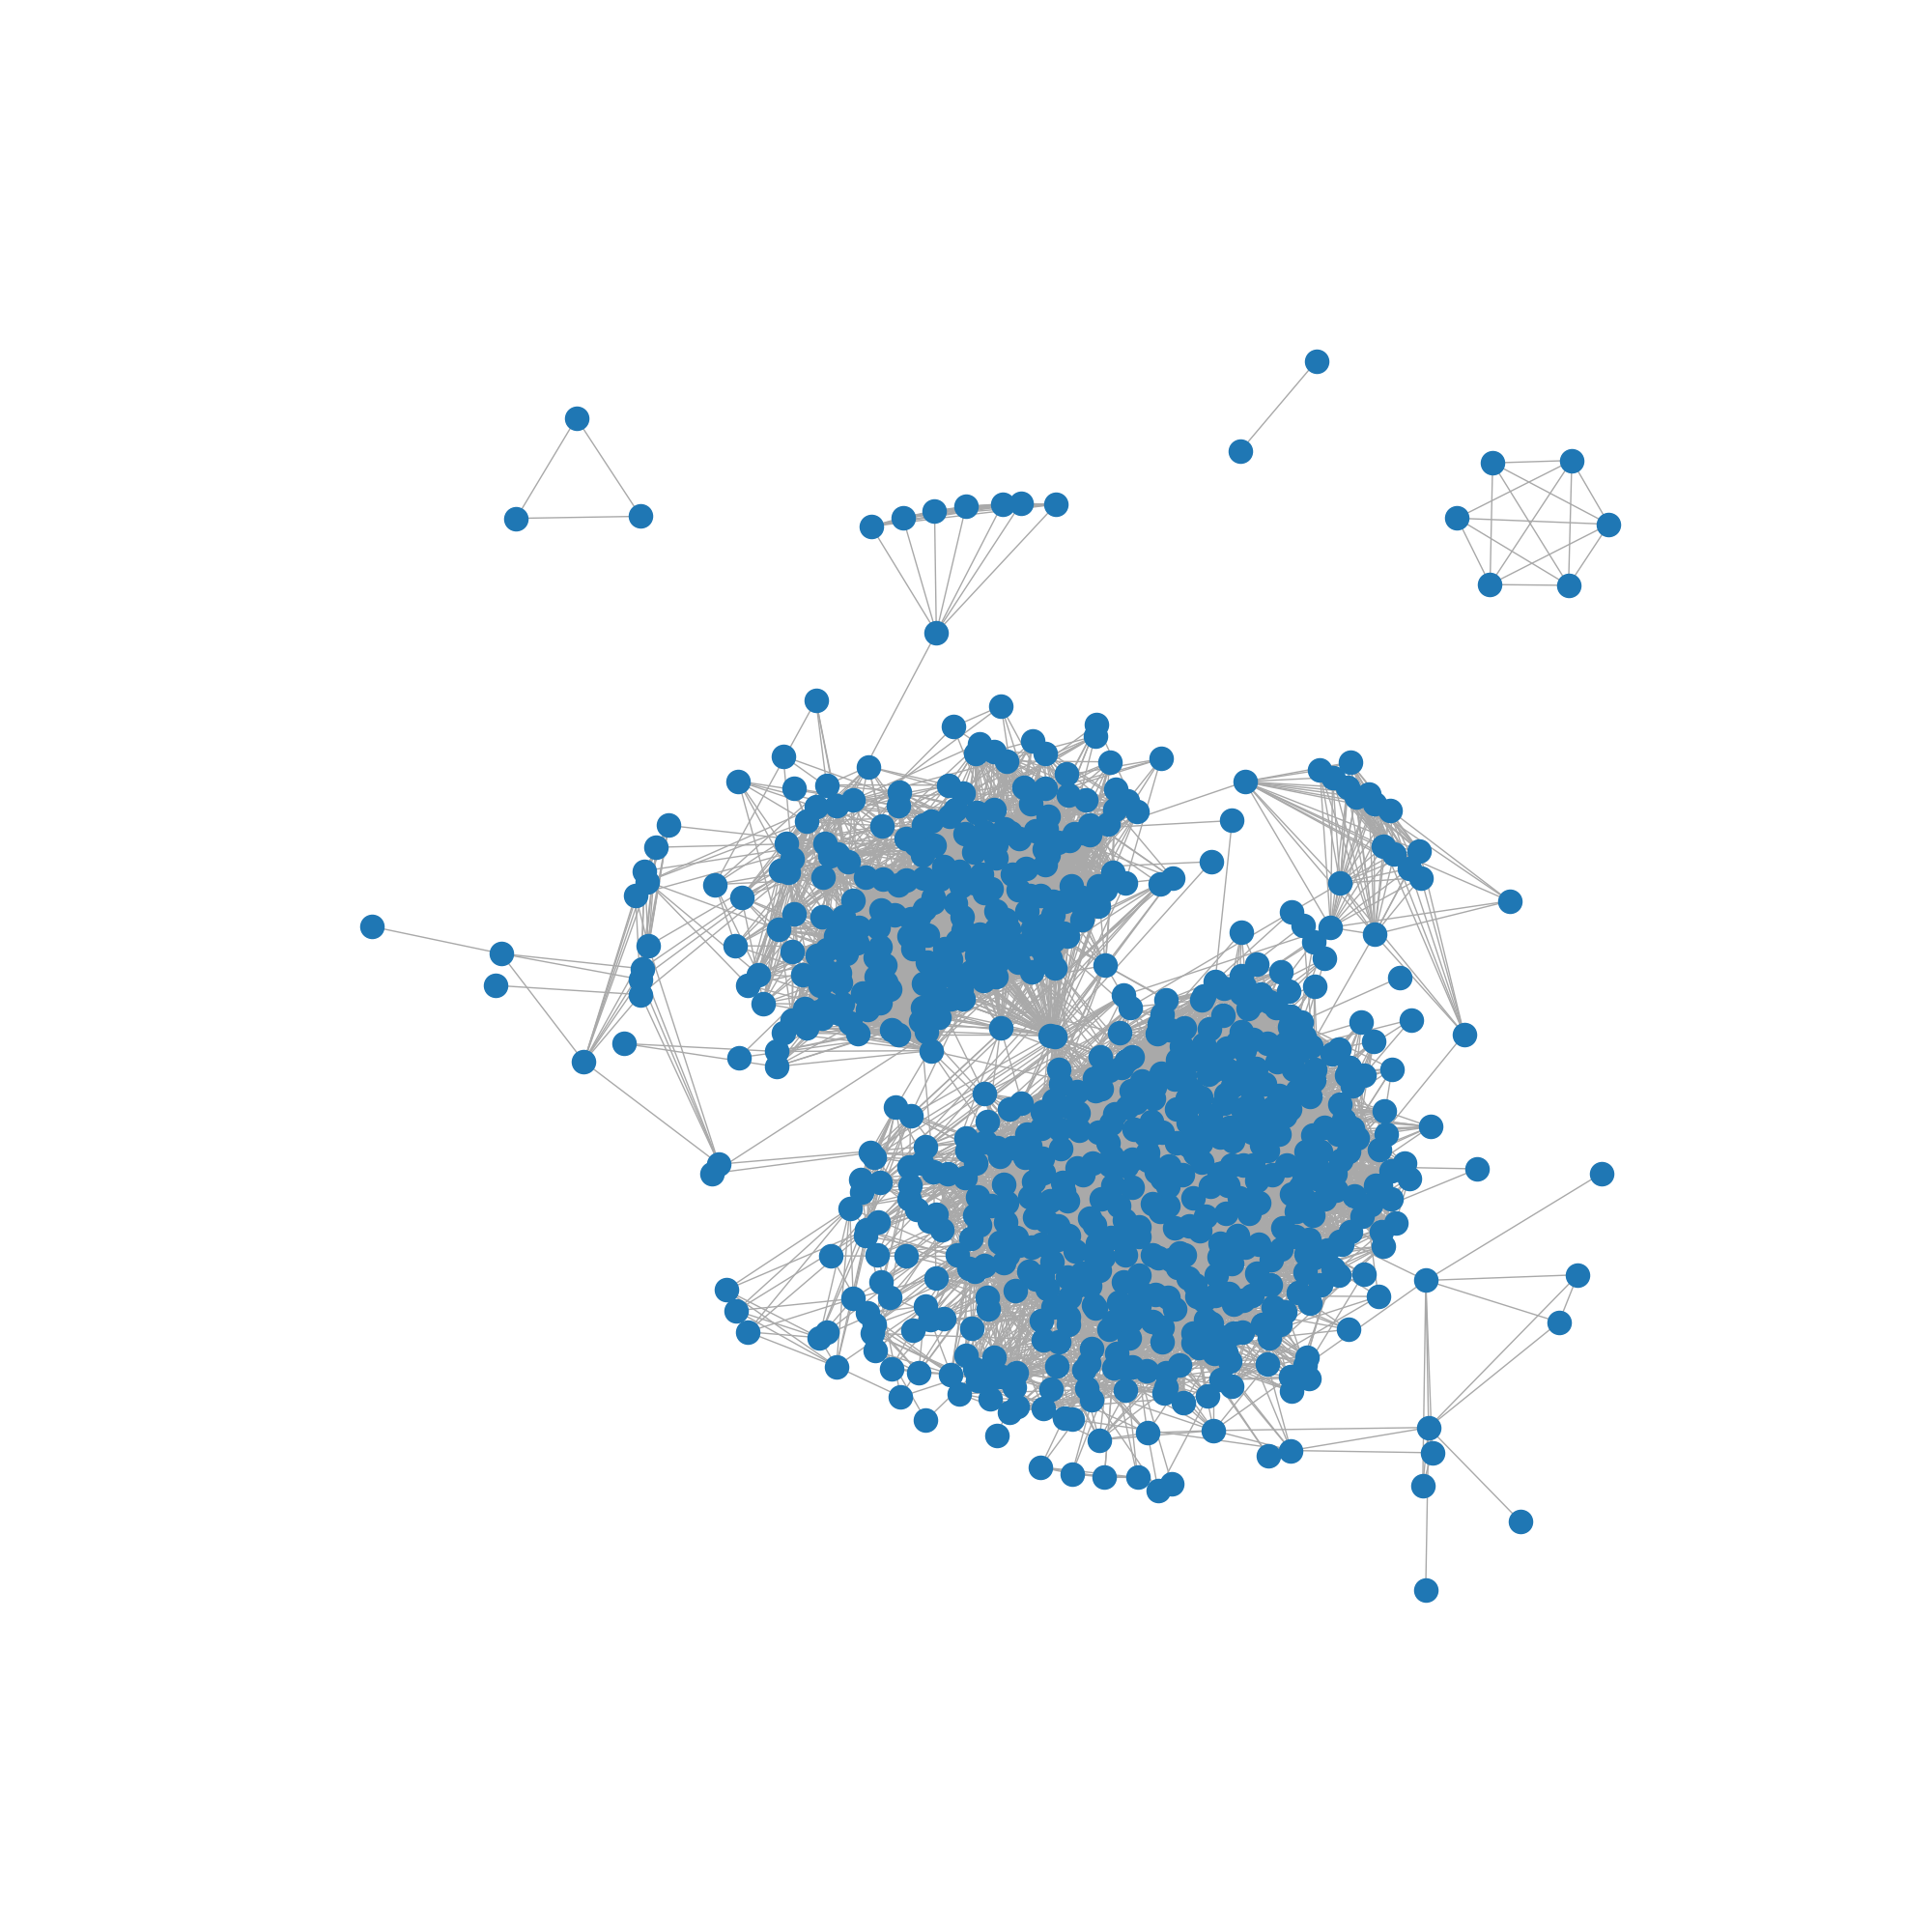
\includegraphics[scale=0.25, trim=200 200 200 200, clip]{/files/src/.media/ego/grafo_facebook.png}
\caption{Una \textit{ego-network} de Facebook compuesta por 786 nodos. Cada vértice representa un individuo, cada arista la existencia de una amistad.} \label{ego_facebook}
\end{figure}

\vspace{1em}
En este análisis\footnote{El script asociado se puede encontrar en \textit{./experimentos/ego\_facebook.py}, los archivos con los resultados  en \textit{./experimentos/resultados/ego-facebook/}.} estimaremos la red `ego' \textbf{E} de la figura (\ref{ego_facebook}.), por medio de la construcción de una matriz de similaridad que utilice el conjunto de atributos \textbf{C} asociados a \textbf{E}\footnote{Por cuestiones de privacidad, los datos están despojados de cualquier referencia a sus cualidades: los nodos y atributos se distinguen por medio de números; los atributos, además, por una parametrización binaria que designa si el nodo porta o no cierta cualidad.}. También, buscaremos reducir su dimensionalidad por medio del análisis de componentes principales.




% === SIMILARIDAD @ ATRIBUTOS === %

\vspace{2em}
\subsection{Matriz de similaridad}

%Queremos generar una aproximación de nuestra red `ego' original \textbf{E} en base a los atributos en \textbf{C} de los usuarios que la componen. Es decir, buscamos un método que nos permita comparar los atributos de dos nodos diferentes y, bajo algún criterio propuesto, conectarlos o no en fin de replicar nuestra red verdadera. 

Queremos generar una aproximación de nuestra red `ego' original, \textbf{E}, a partir de los atributos de los usuarios que la componen, definidos en \textbf{C}. Es decir, buscamos un método que nos permita comparar los atributos de dos nodos diferentes y, bajo algún criterio propuesto, decidir conectarlos o no con el fin de replicar la red verdadera. 

% Intuitivamente, una forma de adivinar si dos usuarios se encuentran conectados en una red es contando la cantidad de atributos que comparten. Se podría pensar que si coinciden en muchos existe una mayor probabilidad de que pertenezcan al mismo círculo, mientras que sino podría ser que ni siquiera se conozcan. Las estructuras que utilizaremos para replicar esta línea de pensamiento son las \textit{matrices de similaridad}, las cuales dado un conjunto de datos $X$ aplican una función a cada par de datos $ij$.

\vspace{1em}
Intuitivamente, una forma de decidir si dos usuarios deberían estar conectados, o no, es contar la cantidad de atributos que comparten. Se podría pensar que si coinciden en muchos, entonces existe una mayor probabilidad que pertenezcan al mismo círculo. Otra forma podría ser medir la distancia, a partir de alguna norma, entre sus vectores de atributos.%Sino, podría ser que ni siquiera se conozcan. 

%\vspace{1em}
%Para replicar esta línea de pensamiento, utilizaremos 
De manera general, podemos pensar en las \textit{matrices de similaridad}. Dado un conjunto de datos $X$, se aplica una función a cada par de elementos $x_i$, $x_j$ tal que:

\vspace{1em}
\begin{equation}
    s_{ij} = f(x_i, x_j)
\end{equation}

%Nuestra tabla de atributos\footnote{La misma puede encontrarse en \textit{./catedra/ego-facebook.feat}.} es tal que la primera columna contiene los tags correspondientes a cada usuario, y el resto de las columnas forman \textbf{C}, donde la $fila_i(\textbf{C})$ son los atributos del usuario $tag_i$. Tomemos entonces nuestra matriz de similaridad $\textbf{S} = \textbf{CC}^{t}$, tal que $\textbf{S}_{ij}$ expresa la similaridad entre la $tag_{i}$ y $tag_{j}$ computando el producto interno de sus respectivos atributos. Con esta información podemos luego proponer diferentes umbrales $u$ entre el menor y mayor valor en \textbf{S}, y establecer que $\textbf{S}_{ij} > u$ indica que los $tag_{i}$ y $tag_{j}$ están conectados en nuestra aproximación. 

\vspace{2em}
En nuestro caso, trabajaremos con una tabla de atributos\footnote{La misma se puede encontrar en \textit{./catedra/ego-facebook.feat}. Dado que la red original y esta tabla no comparten todos sus nodos, se realizó un proceso de filtrado y limpieza. Las versiones corregidas se encuentran en \textit{./experimentos/resultados/ego-facebook/}.} cuya primer columna contiene las etiquetas ($tags$) de cada nodo en la red, y el resto de las columnas forman \textbf{C} ---donde la $\text{\textit{fila}}_i(\textbf{C})$ representa los atributos del usuario definido por la etiqueta $i$---. A partir de estos datos, definiremos la matriz de similaridad de la siguiente forma:

\vspace{1em}
\begin{equation}
    \mathbf{S} = \mathbf{C}\ \mathbf{C}^{t}
\end{equation}

\vspace{1em}
\noindent donde $s_{ij}$ expresa la similaridad entre el nodo $i$ y el $j$ por medio del producto interno de sus respectivos vectores de atributos. 

\vspace{1em}
Con esta información propondremos diferentes umbrales $u$ en el rango $[min(\mathbf{S}),\ max(\mathbf{S}))$ que servirán como criterio para aproximar \textbf{E}. Si $s_{ij} > u$, entonces los nodos $i$ y $j$ estarán conectados. 

%Procedemos a mostrar los resultados obtenidos. Tomando $u \in [min{\textbf{S}_{ij}},\ max{\textbf{S}_{ij}}) = [0, 22)$, $u \in \mathbb{Z}$, obtuvimos 22 diferentes aproximaciones de \textbf{E}.

\vspace{2em}
\noindent \textsc{Resultados}. Vemos que cada elemento $s_{ij}$ es entero, por producto punto de enteros, y $[min(\mathbf{S}),\ max(\mathbf{S})) = [0, 22)$. A partir de estas observaciones aproximamos \textbf{E} por medio de 22 umbrales distintos: $[0,\ 1,\ ...,\ 22]$. La figura (\ref{grafos_aproximados}.) muestra una representación de los grafos obtenidos más significativos. 

%Obsérvese que cuanto más alto sea el umbral, menores conexiones tendremos en nuestro grafo aproximado. En particular, con $u = 0$ se obtiene un grafo donde todos los usuarios están conectados entre sí, y con $u > 12$ grafos con ninguna arista. Nos enfocaremos entonces con los asociados a $u \in [0, 12]$, ya que son los que revelan información de interés.

\vspace{1em}
Observamos que cuanto mayor sea el umbral, menos conexiones tendremos en nuestra aproximación. En particular, con $u = 0$ se obtiene un grafo donde casi todos los usuarios están conectados entre sí, y con $u > 12$ obtenemos un grafo sin ninguna arista. Nos enfocaremos entonces en los grafos asociados a $u \in [0, 12]$, ya que estos son los que revelan la mayor cantidad de información. 

\vspace{1em}
\begin{figure}[!htbp]
    \centering
    \subfloat[$u = 0$]{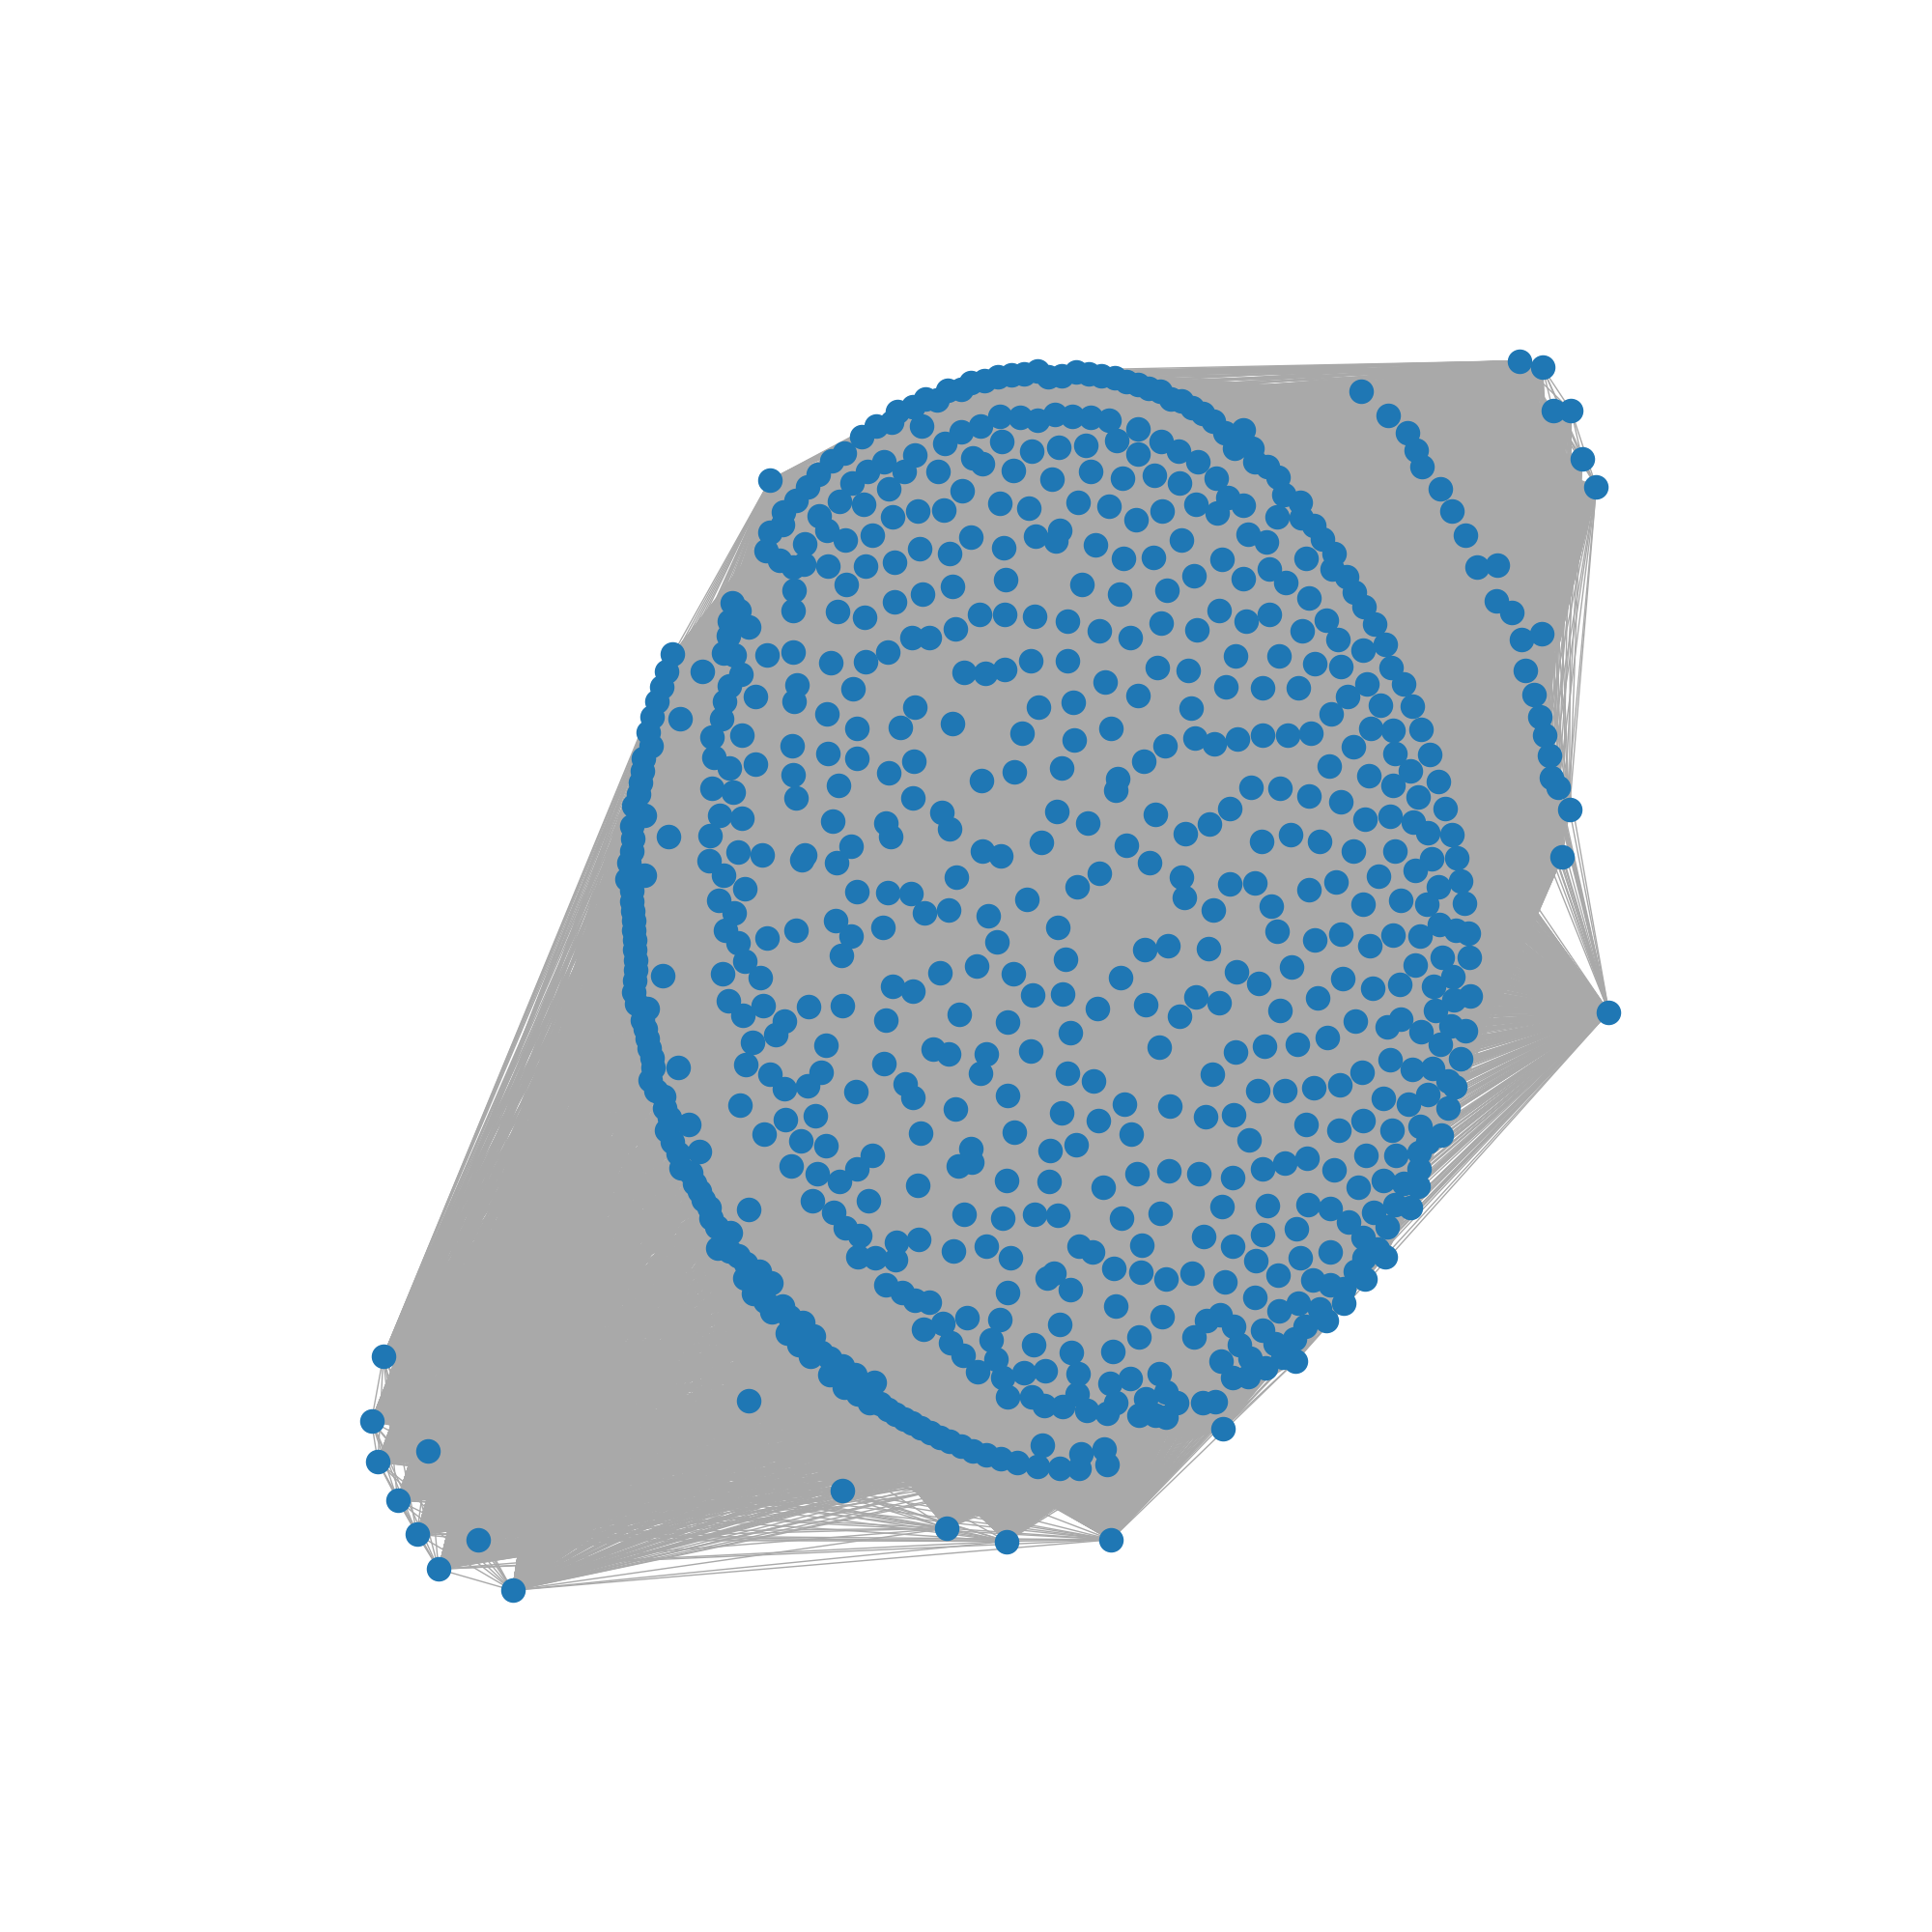
\includegraphics[width=.25\textwidth]{/files/src/.media/ego/grafo_1.png}}\hfill
    \subfloat[$u = 1$]{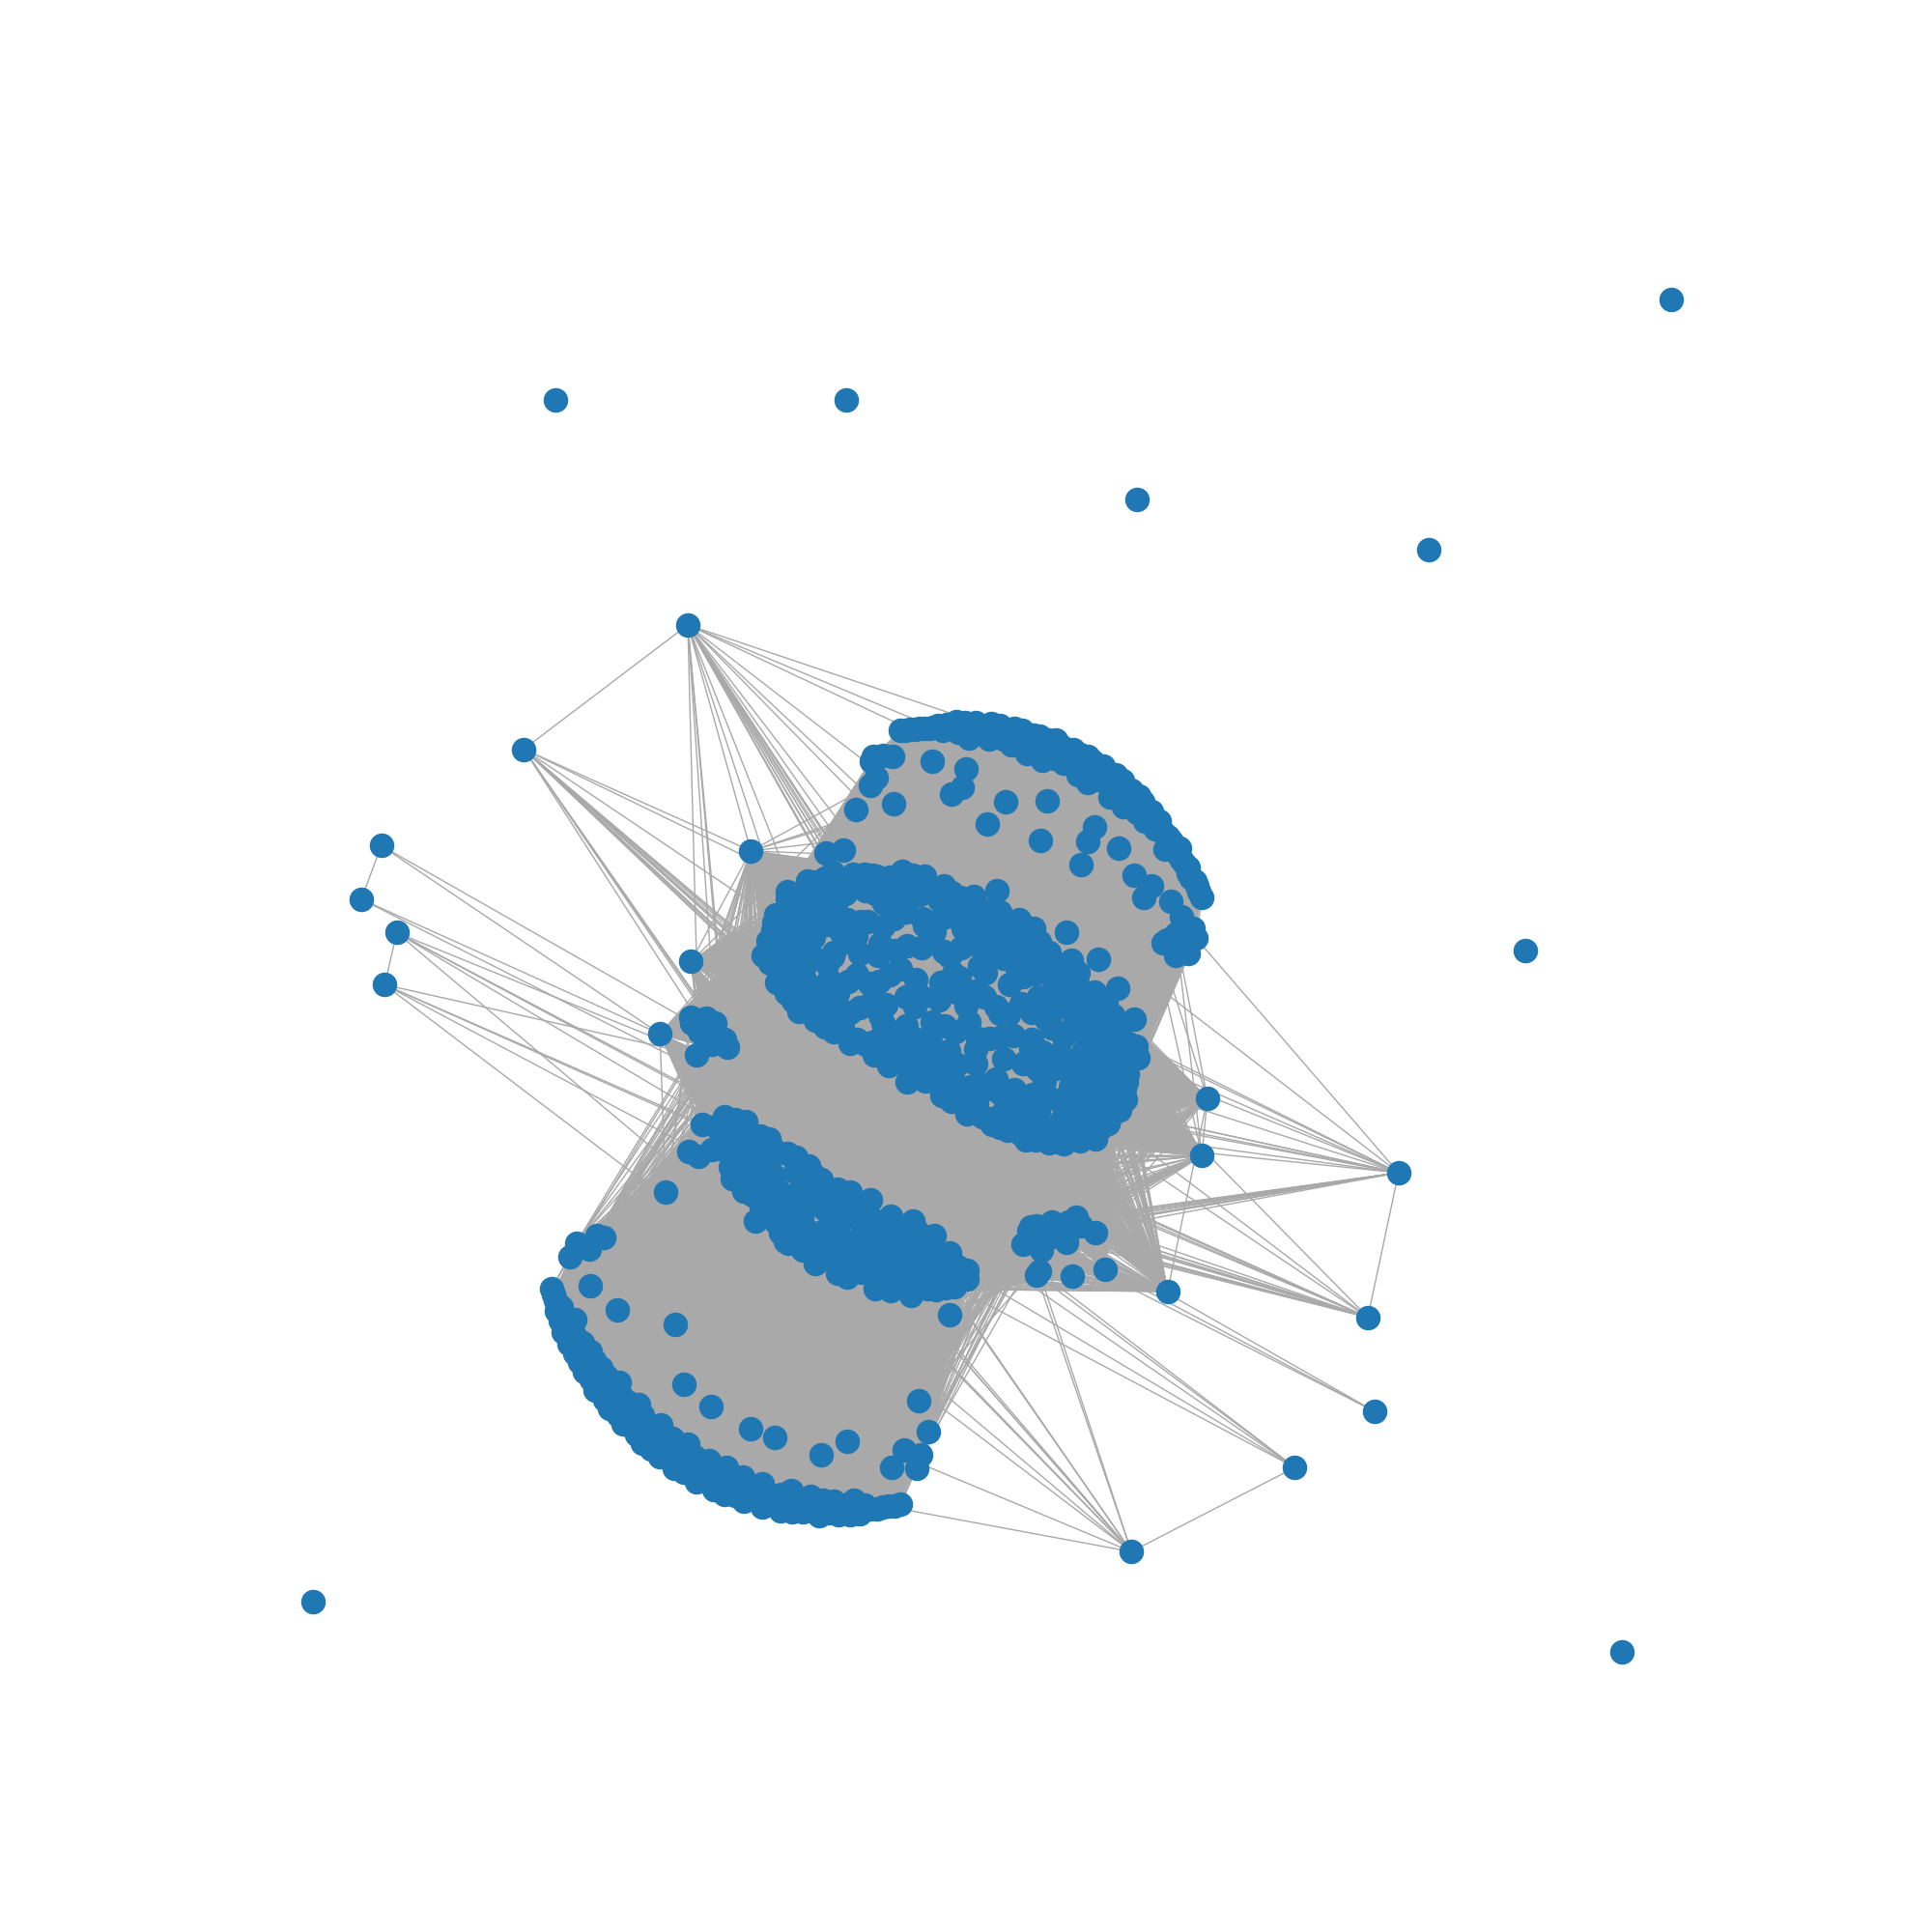
\includegraphics[width=.25\textwidth]{/files/src/.media/ego/grafo_2.png}}\hfill
    \subfloat[$u = 2$]{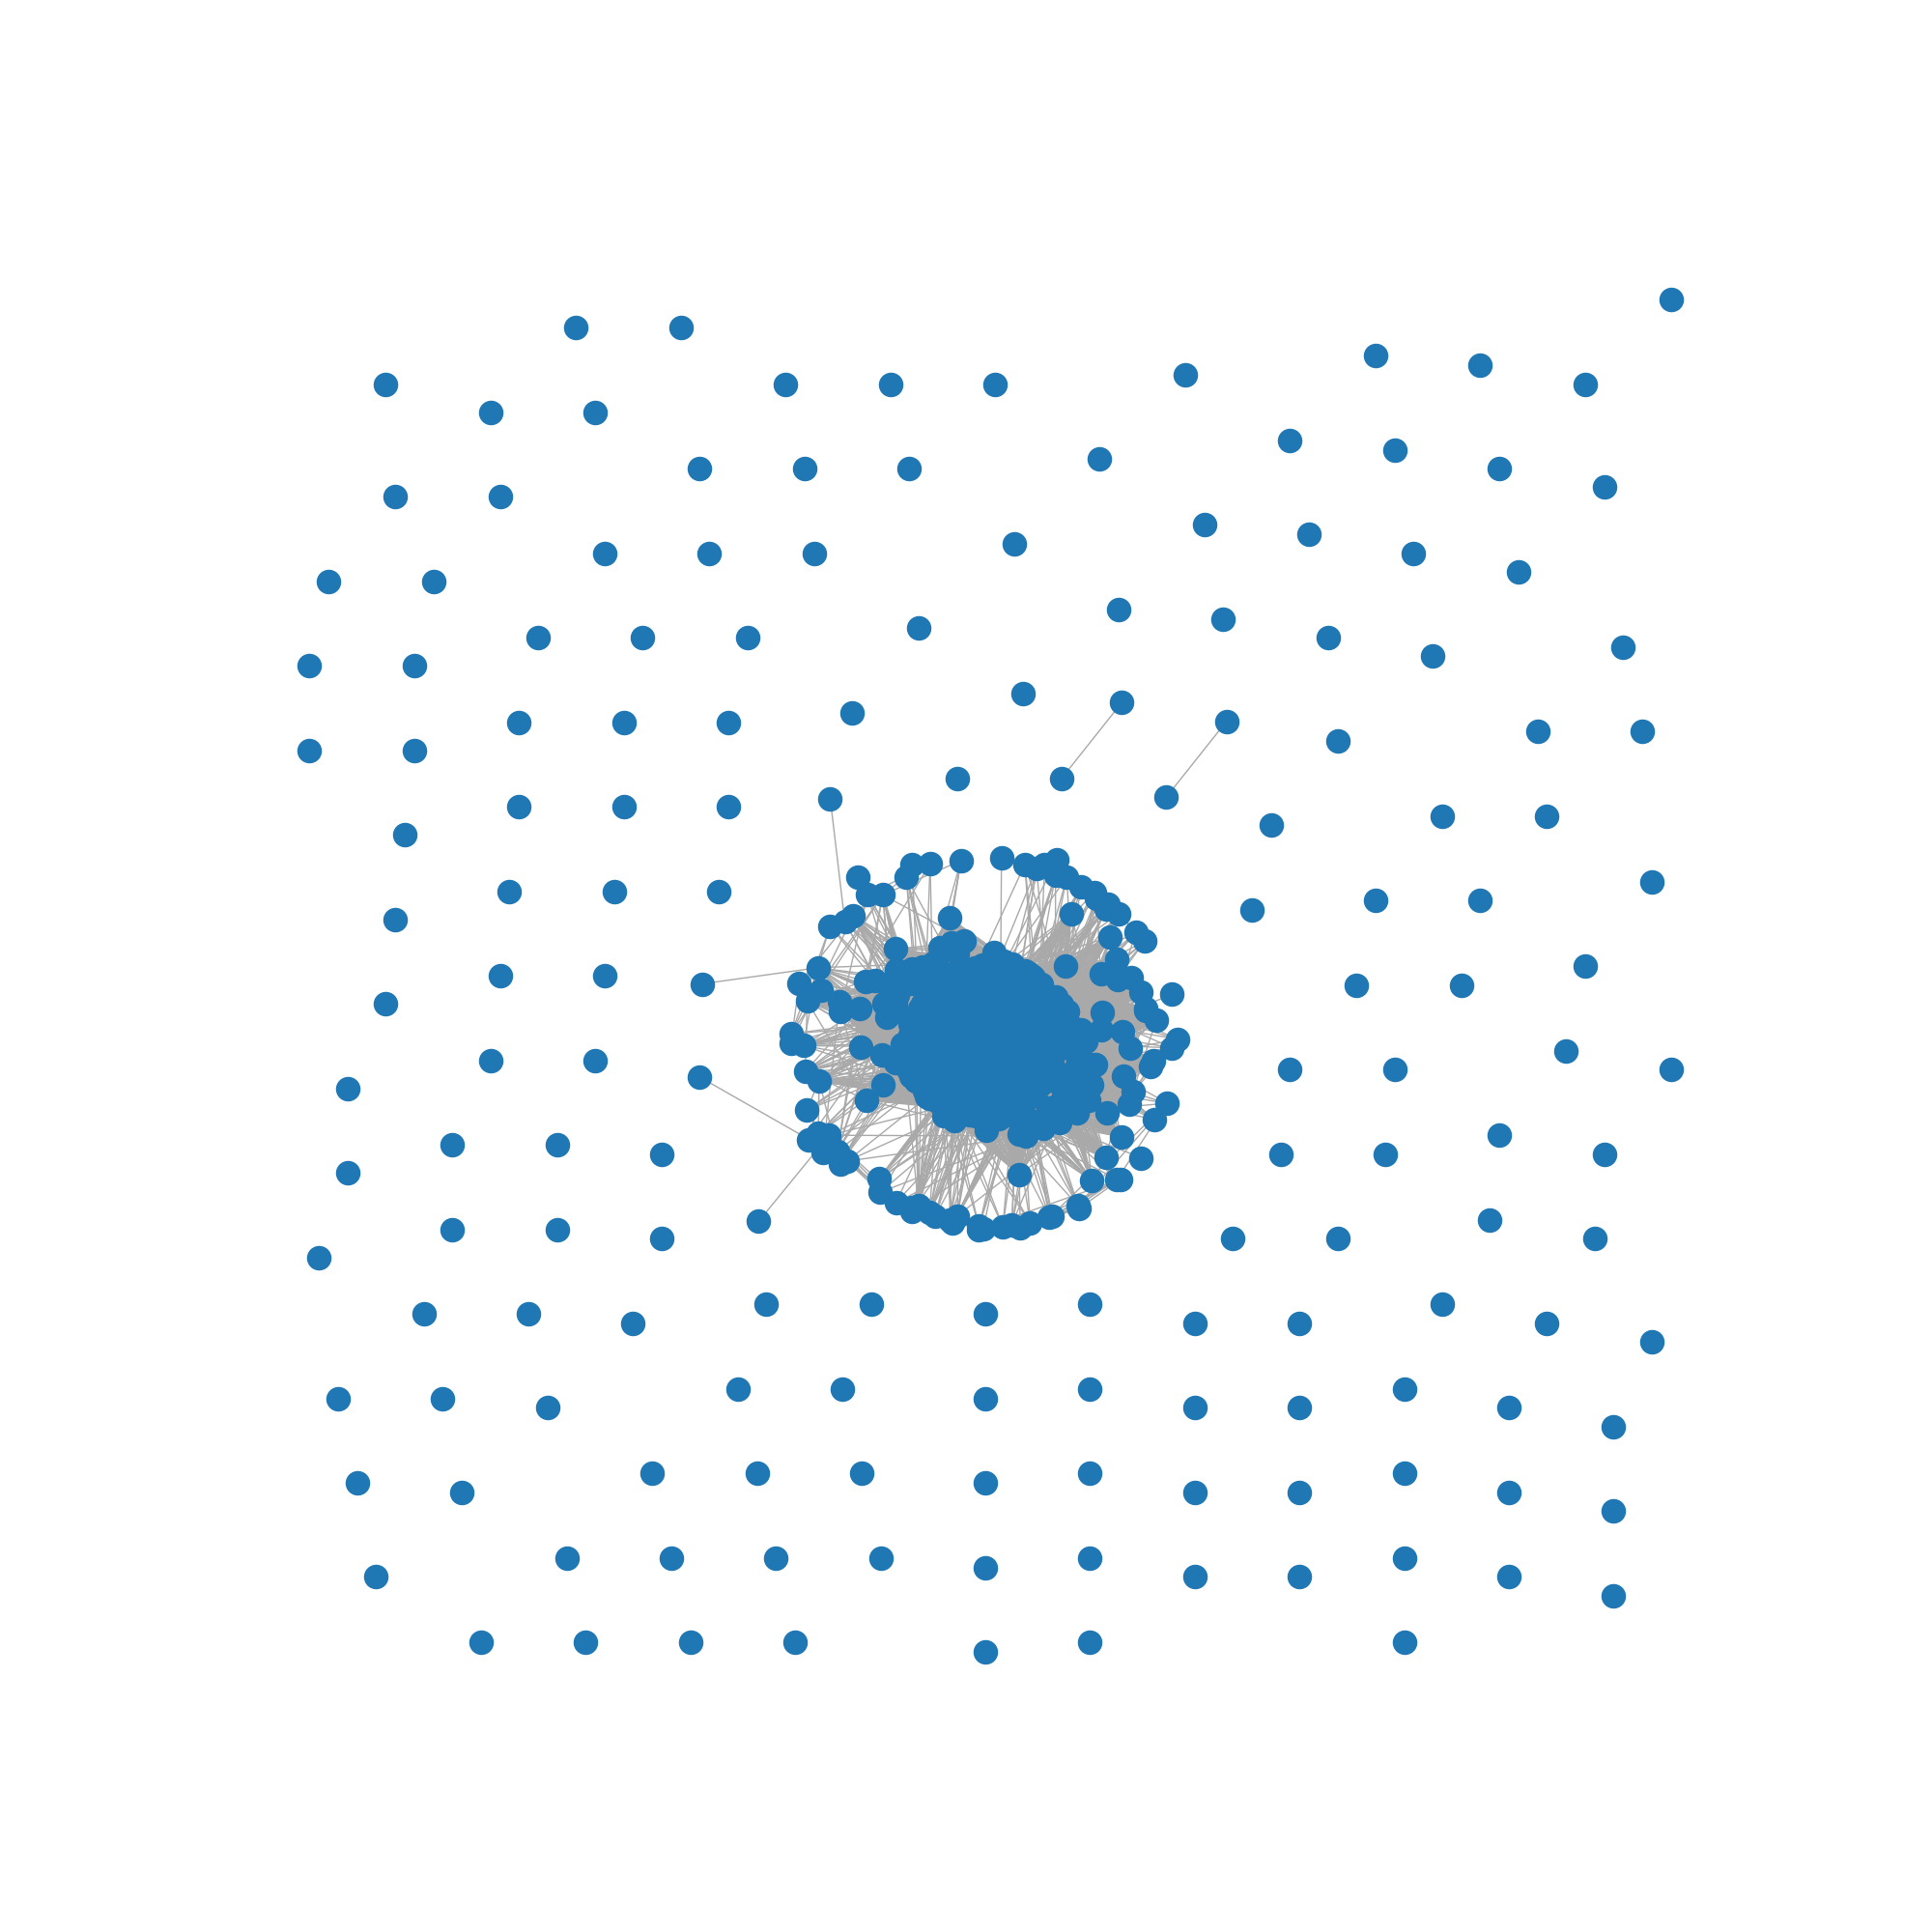
\includegraphics[width=.25\textwidth]{/files/src/.media/ego/grafo_3.png}}\hfill
    \subfloat[$u = 3$]{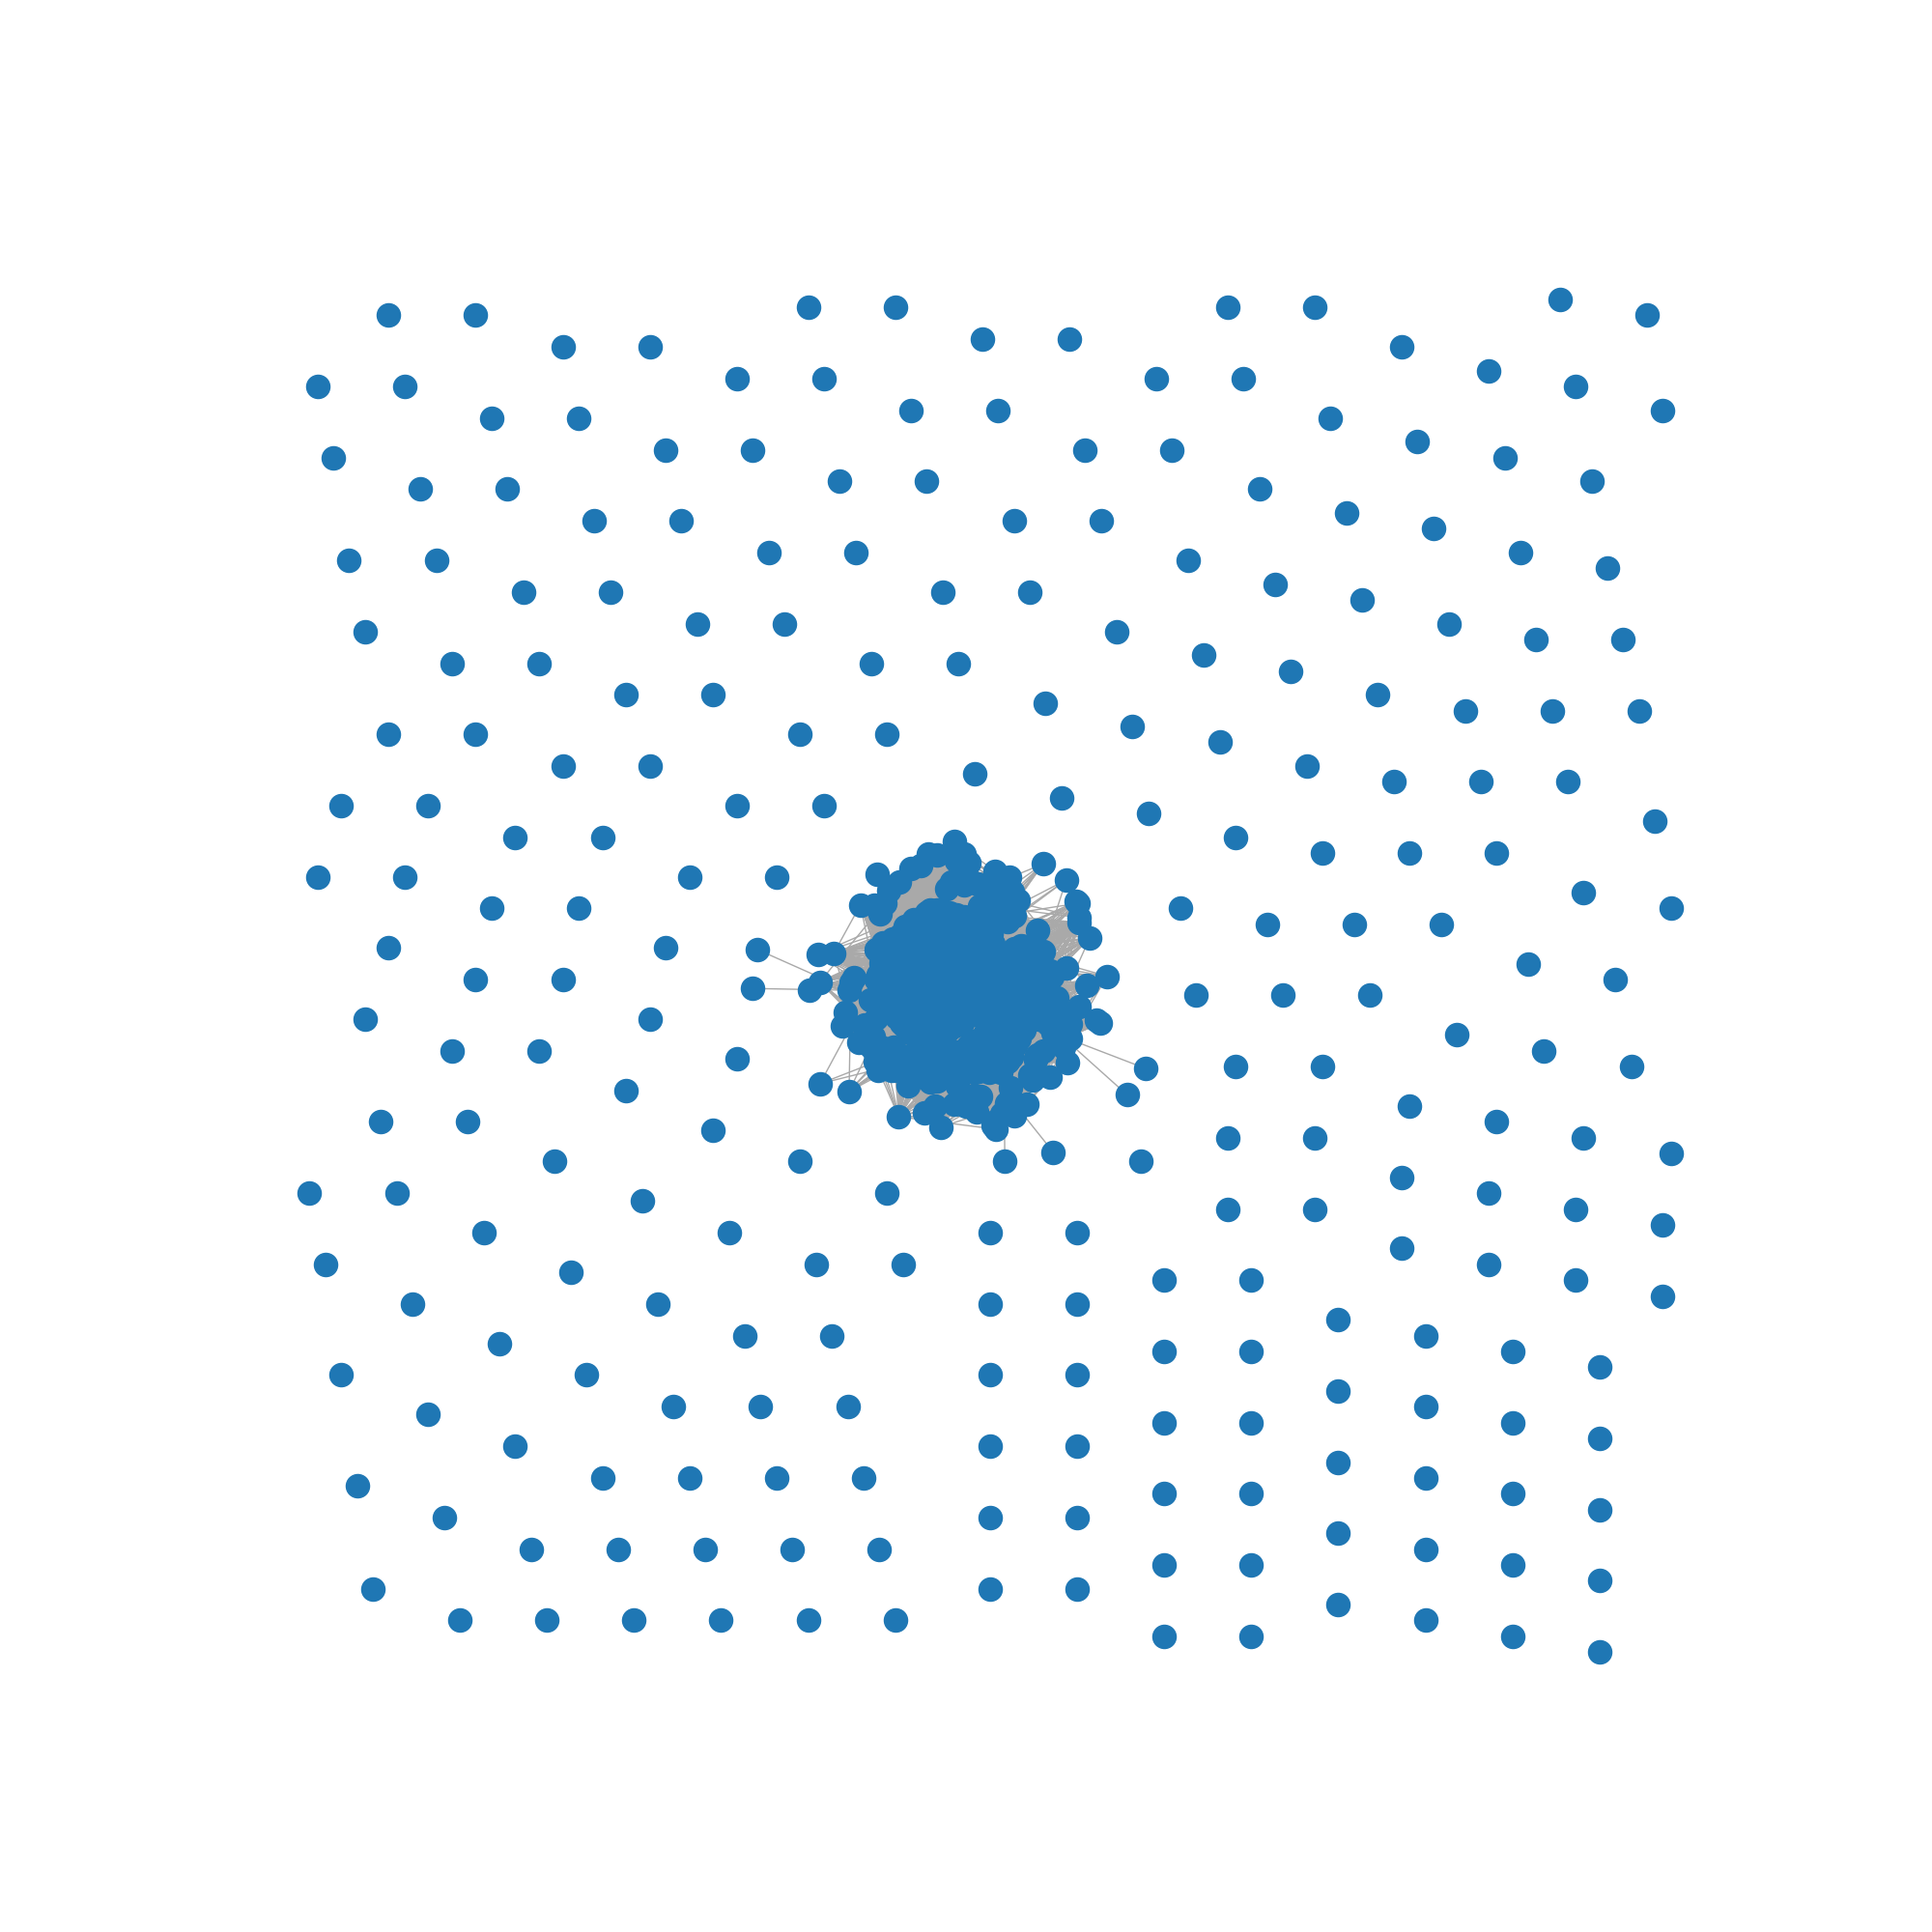
\includegraphics[width=.25\textwidth]{/files/src/.media/ego/grafo_4.png}}\hfill
% \end{figure}
% \begin{figure}[!htbp]
%     \ContinuedFloat
%     \centering
    \\[\smallskipamount]
    \subfloat[$u = 4$]{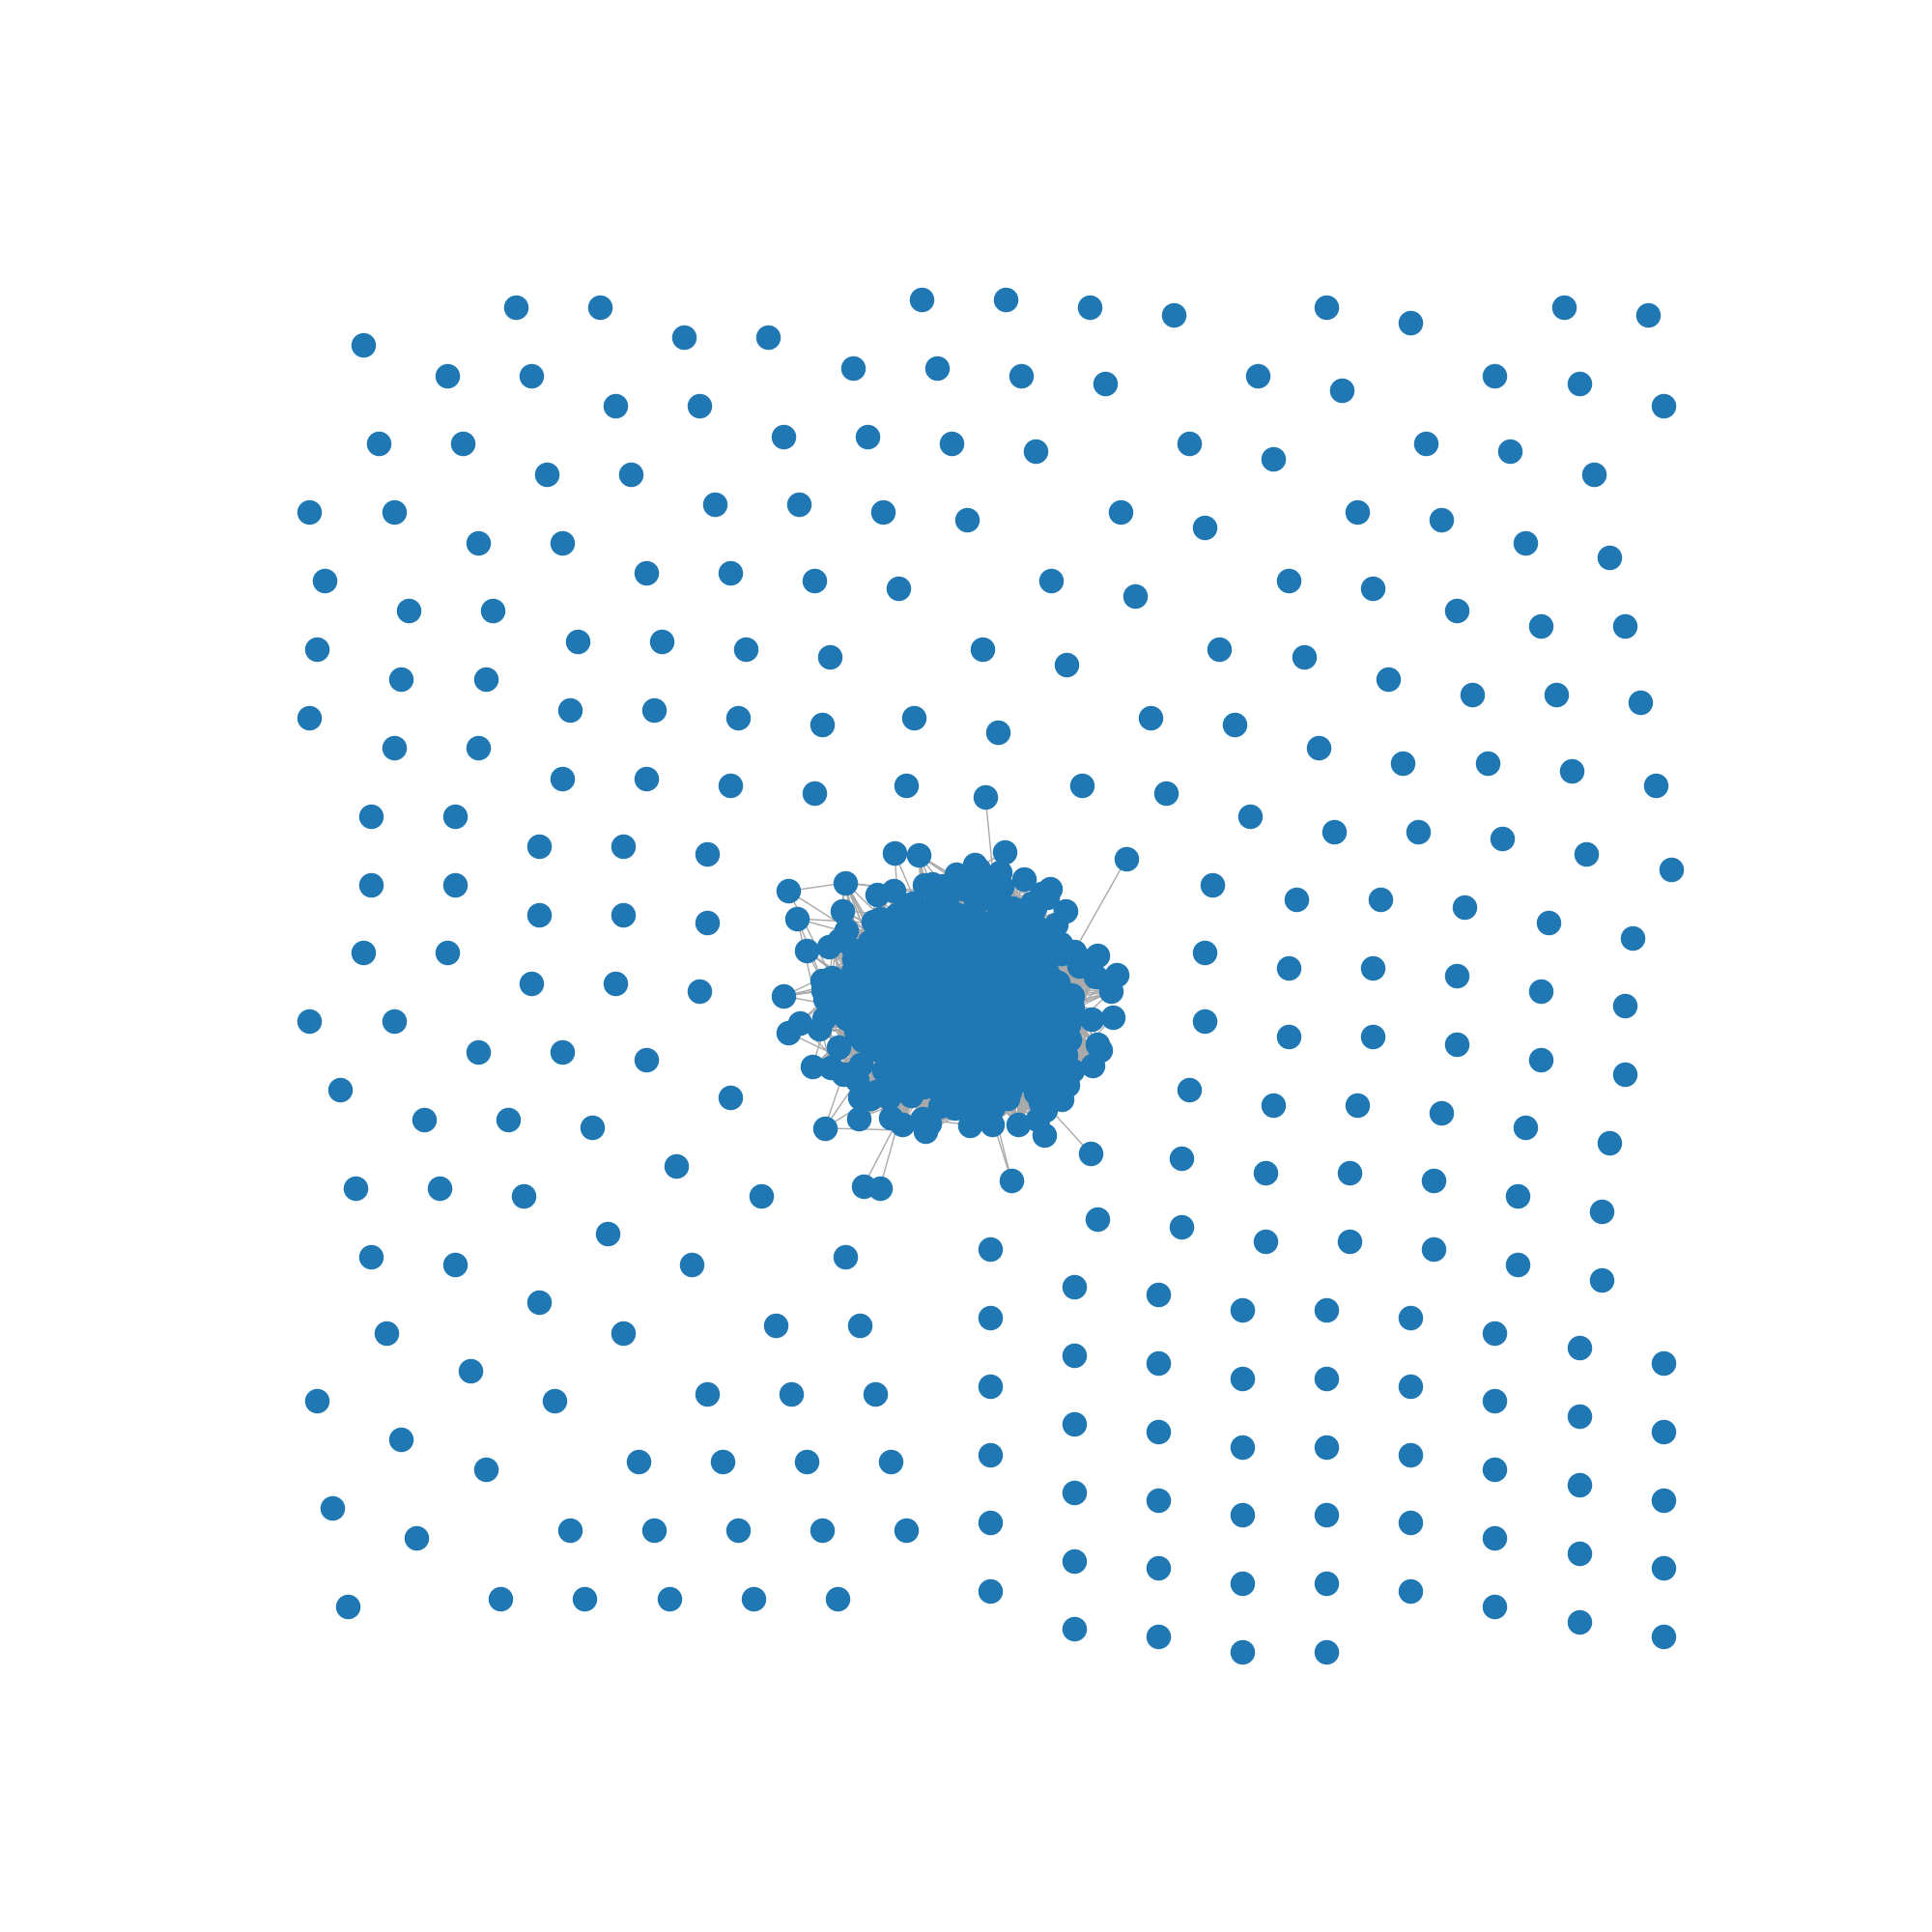
\includegraphics[width=.25\textwidth]{/files/src/.media/ego/grafo_5.png}}\hfill
    \subfloat[$u = 5$]{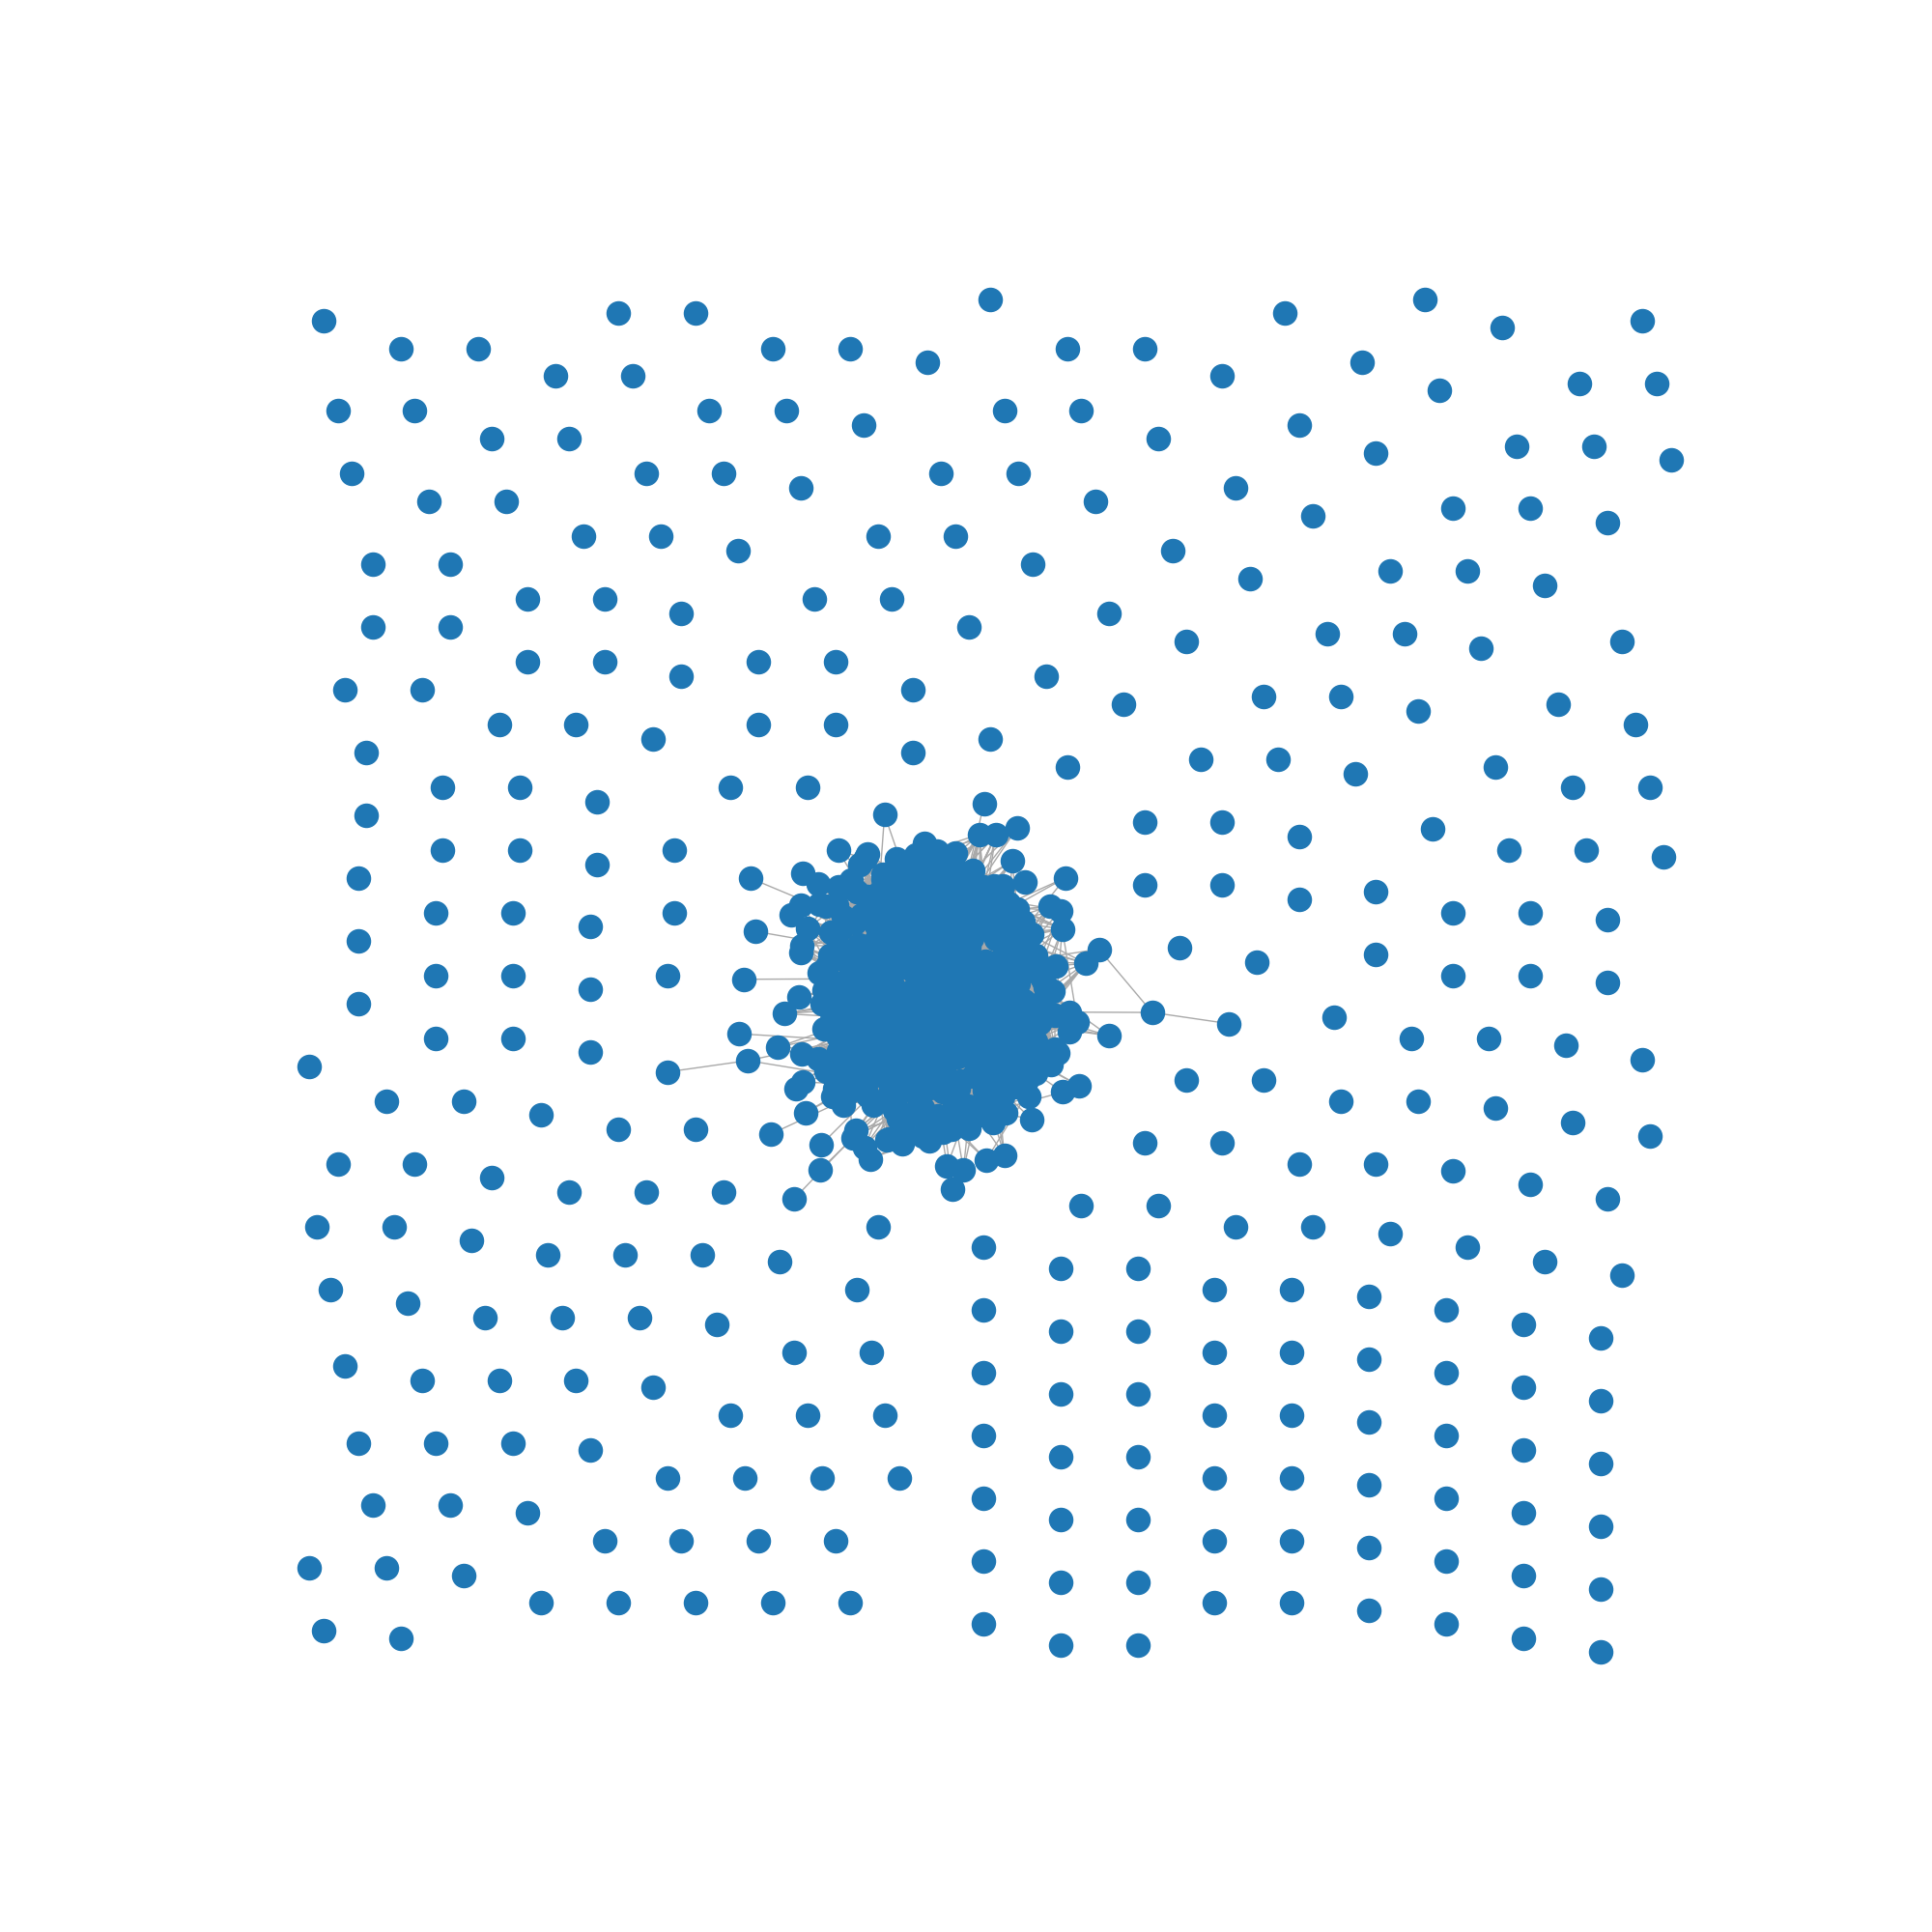
\includegraphics[width=.25\textwidth]{/files/src/.media/ego/grafo_6.png}}\hfill
    \subfloat[$u = 6$]{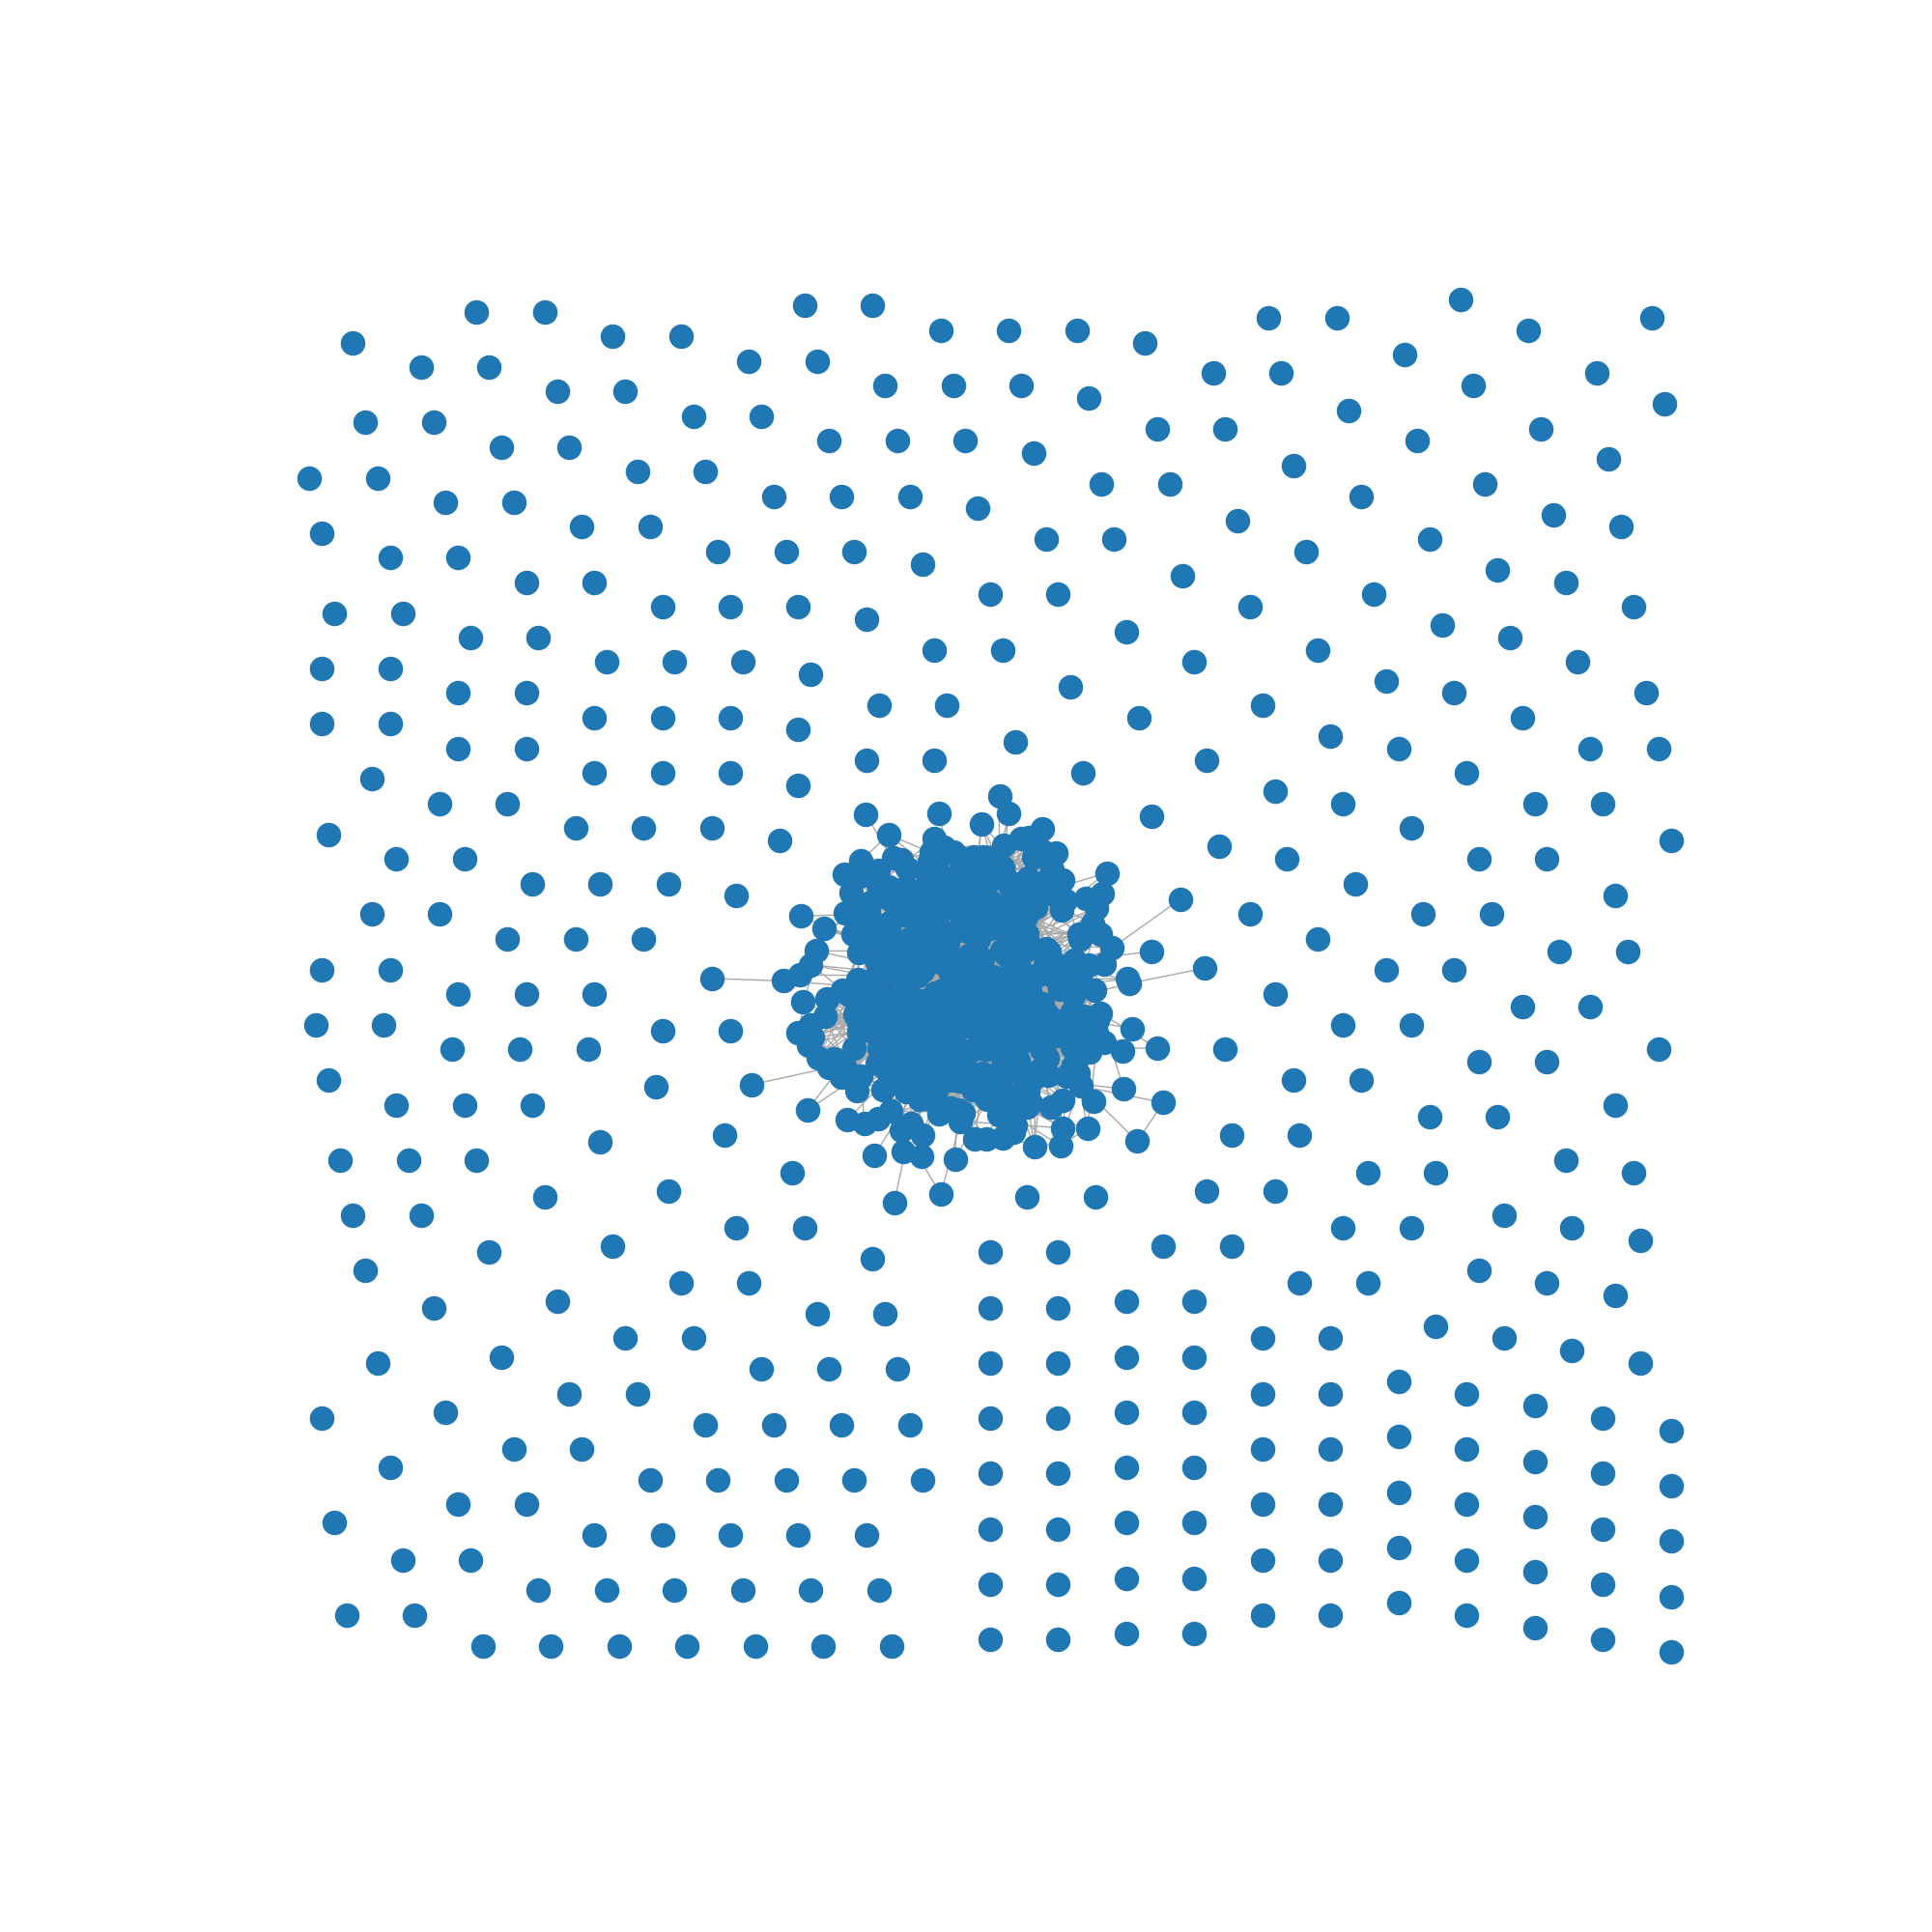
\includegraphics[width=.25\textwidth]{/files/src/.media/ego/grafo_7.png}}\hfill
    \subfloat[$u = 7$]{
\includegraphics[width=.25\textwidth]{/files/src/.media/ego/grafo_8.png}}\hfill    
    \\[\smallskipamount]
    \subfloat[$u = 8$]{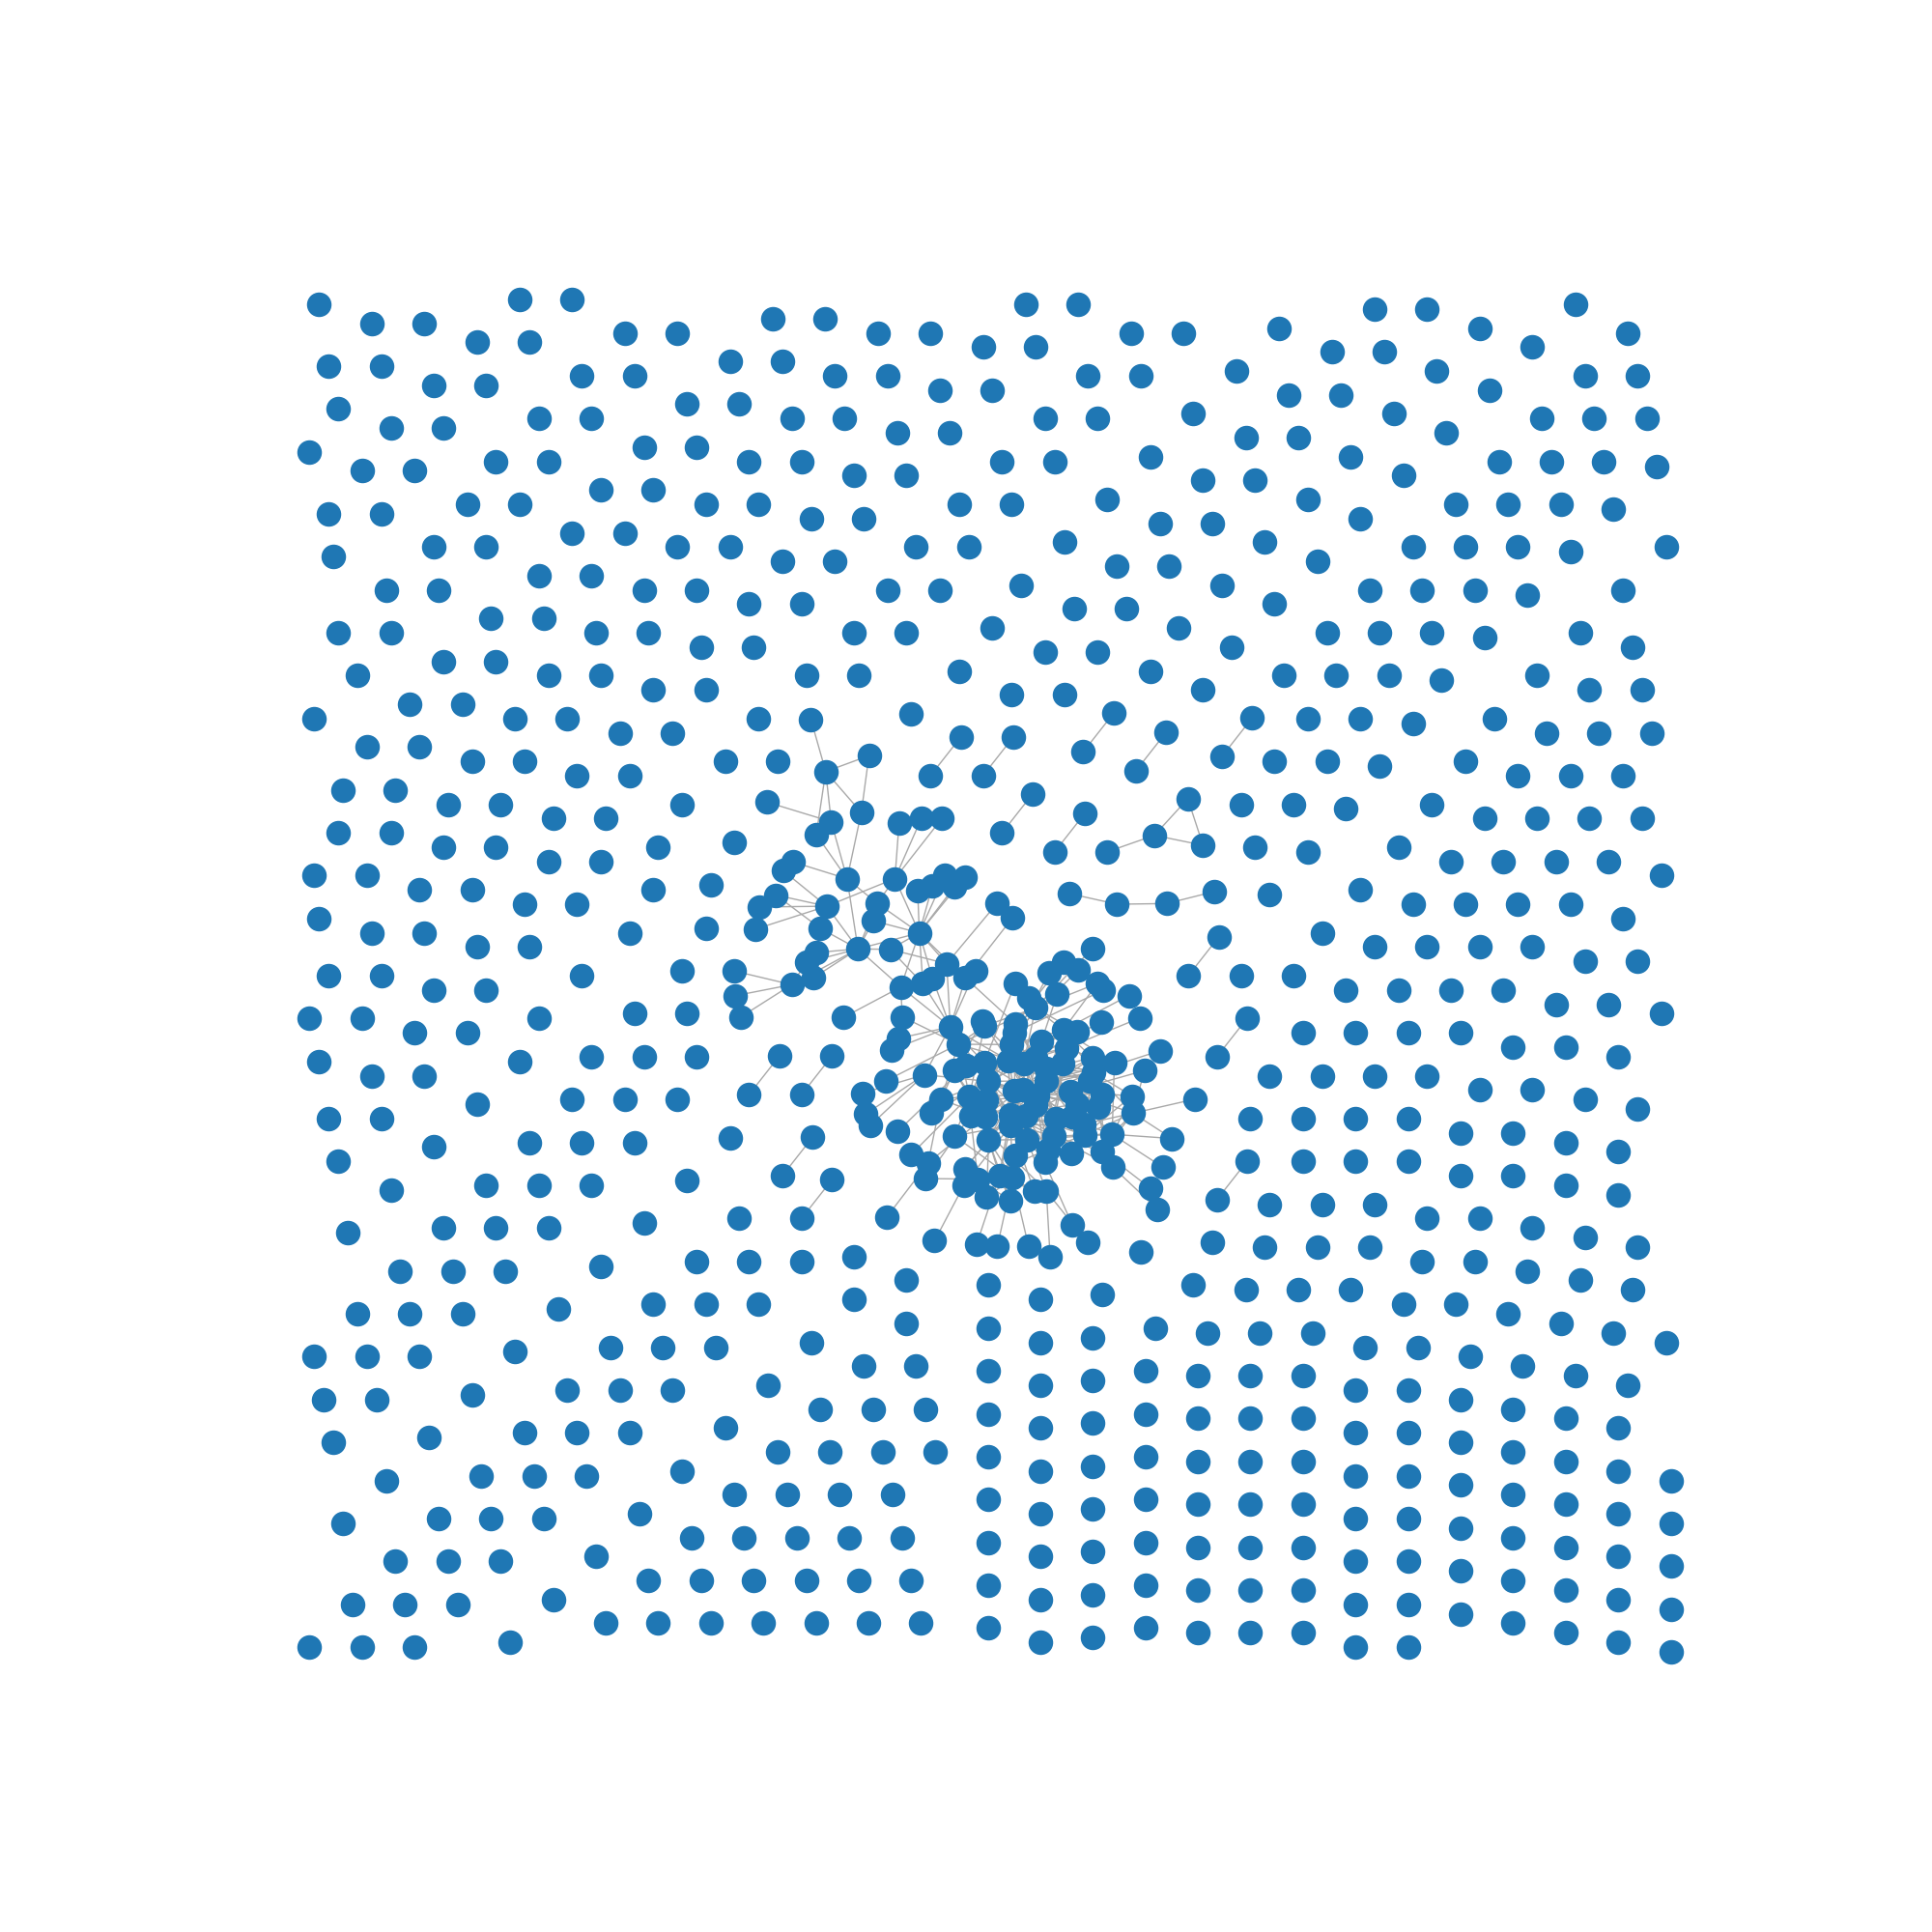
\includegraphics[width=.25\textwidth]{/files/src/.media/ego/grafo_9.png}}\hfill
    \subfloat[$u = 9$]{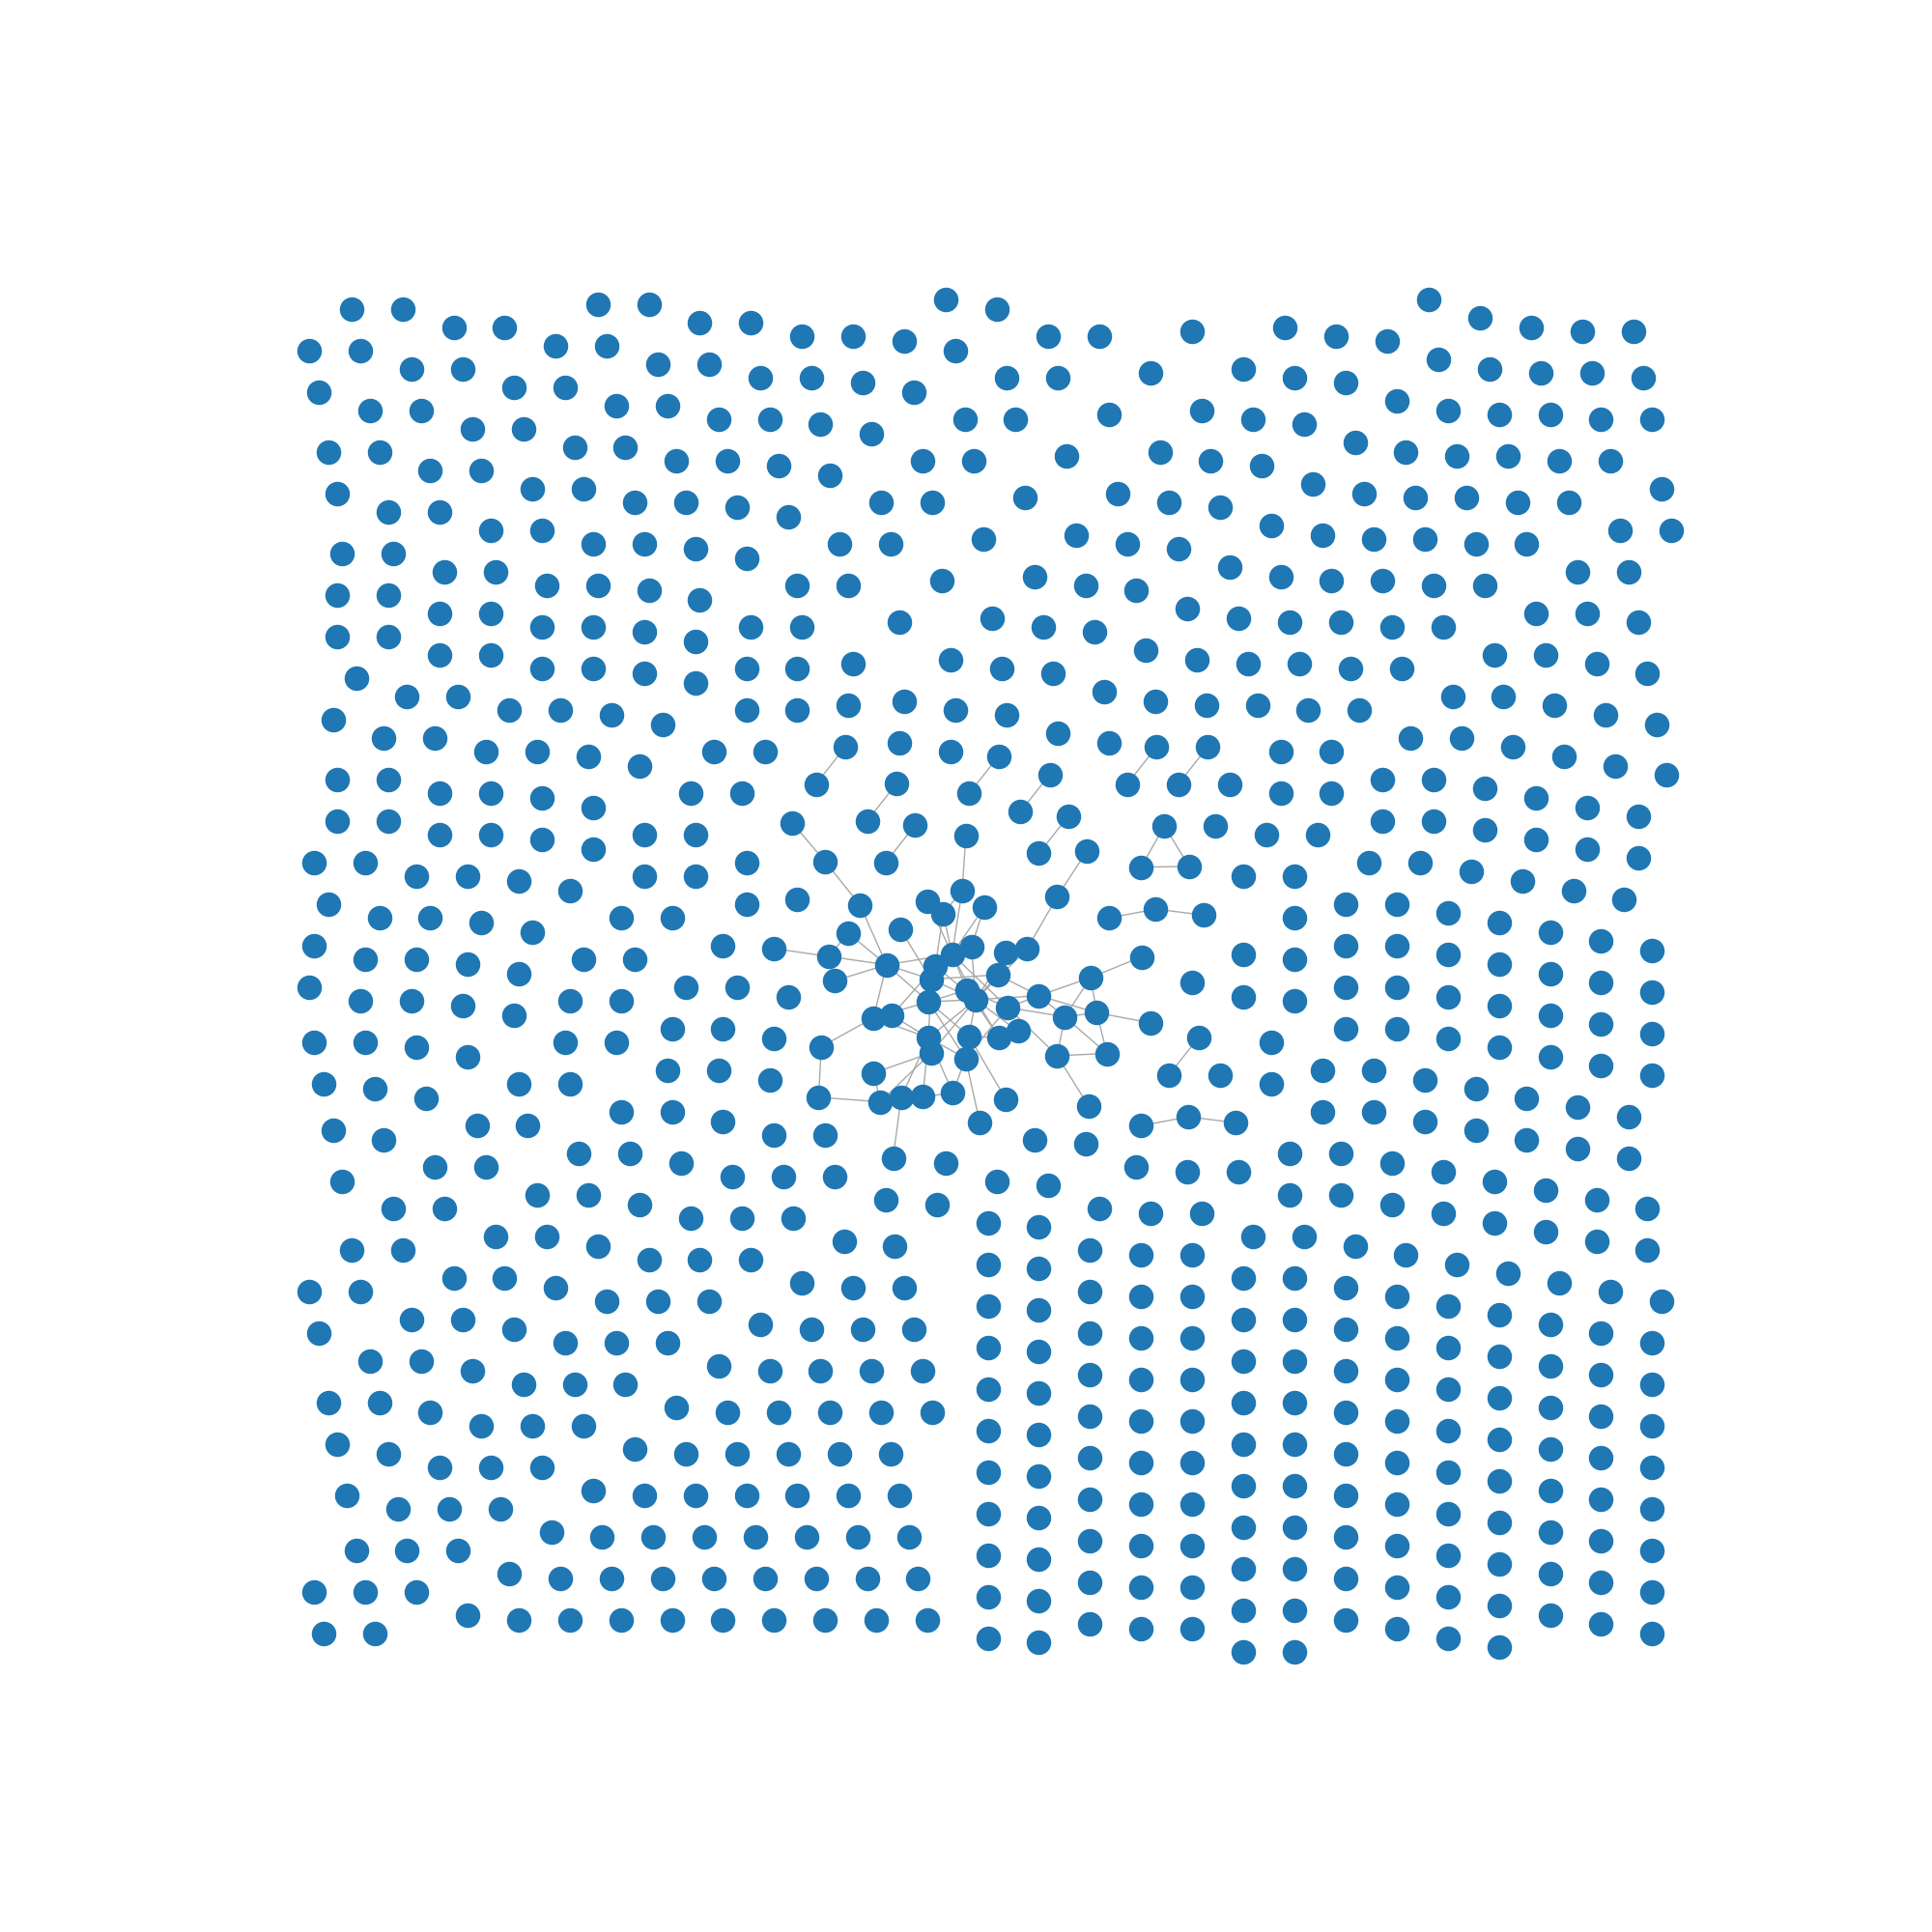
\includegraphics[width=.25\textwidth]{/files/src/.media/ego/grafo_10.png}}\hfill
    \subfloat[$u = 10$]{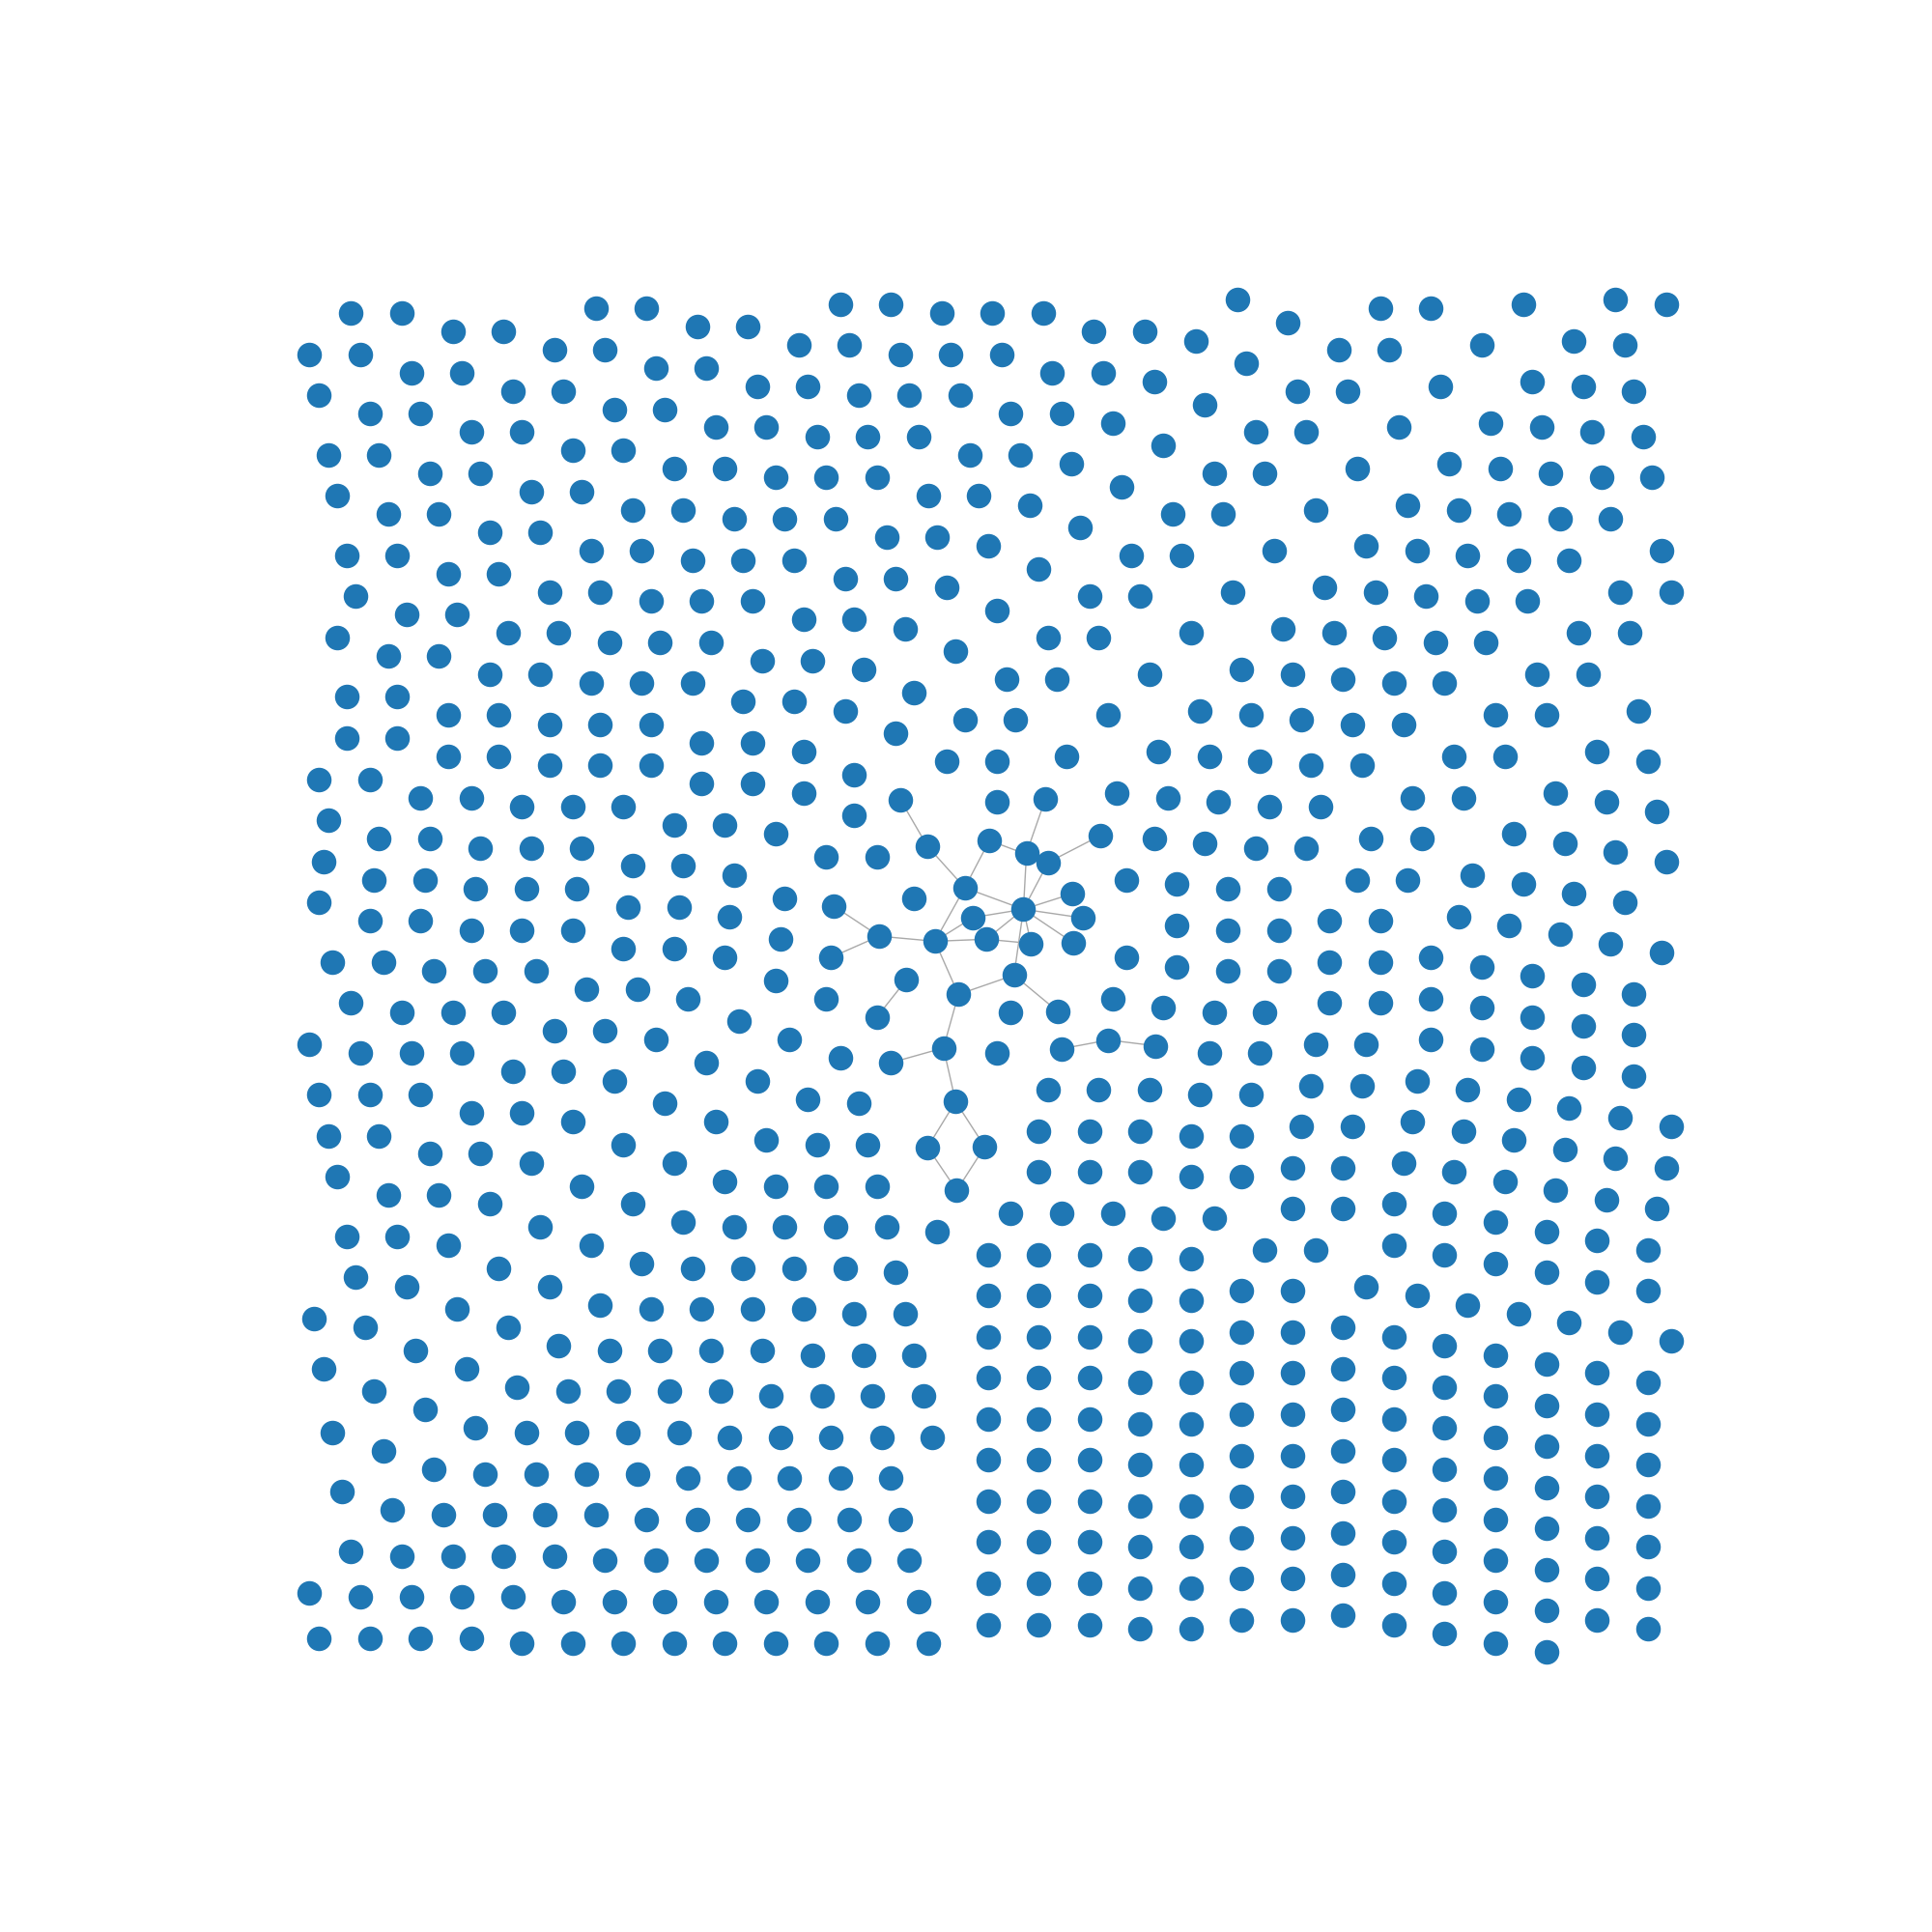
\includegraphics[width=.25\textwidth]{/files/src/.media/ego/grafo_11.png}}\hfill
    \subfloat[$u = 11$]{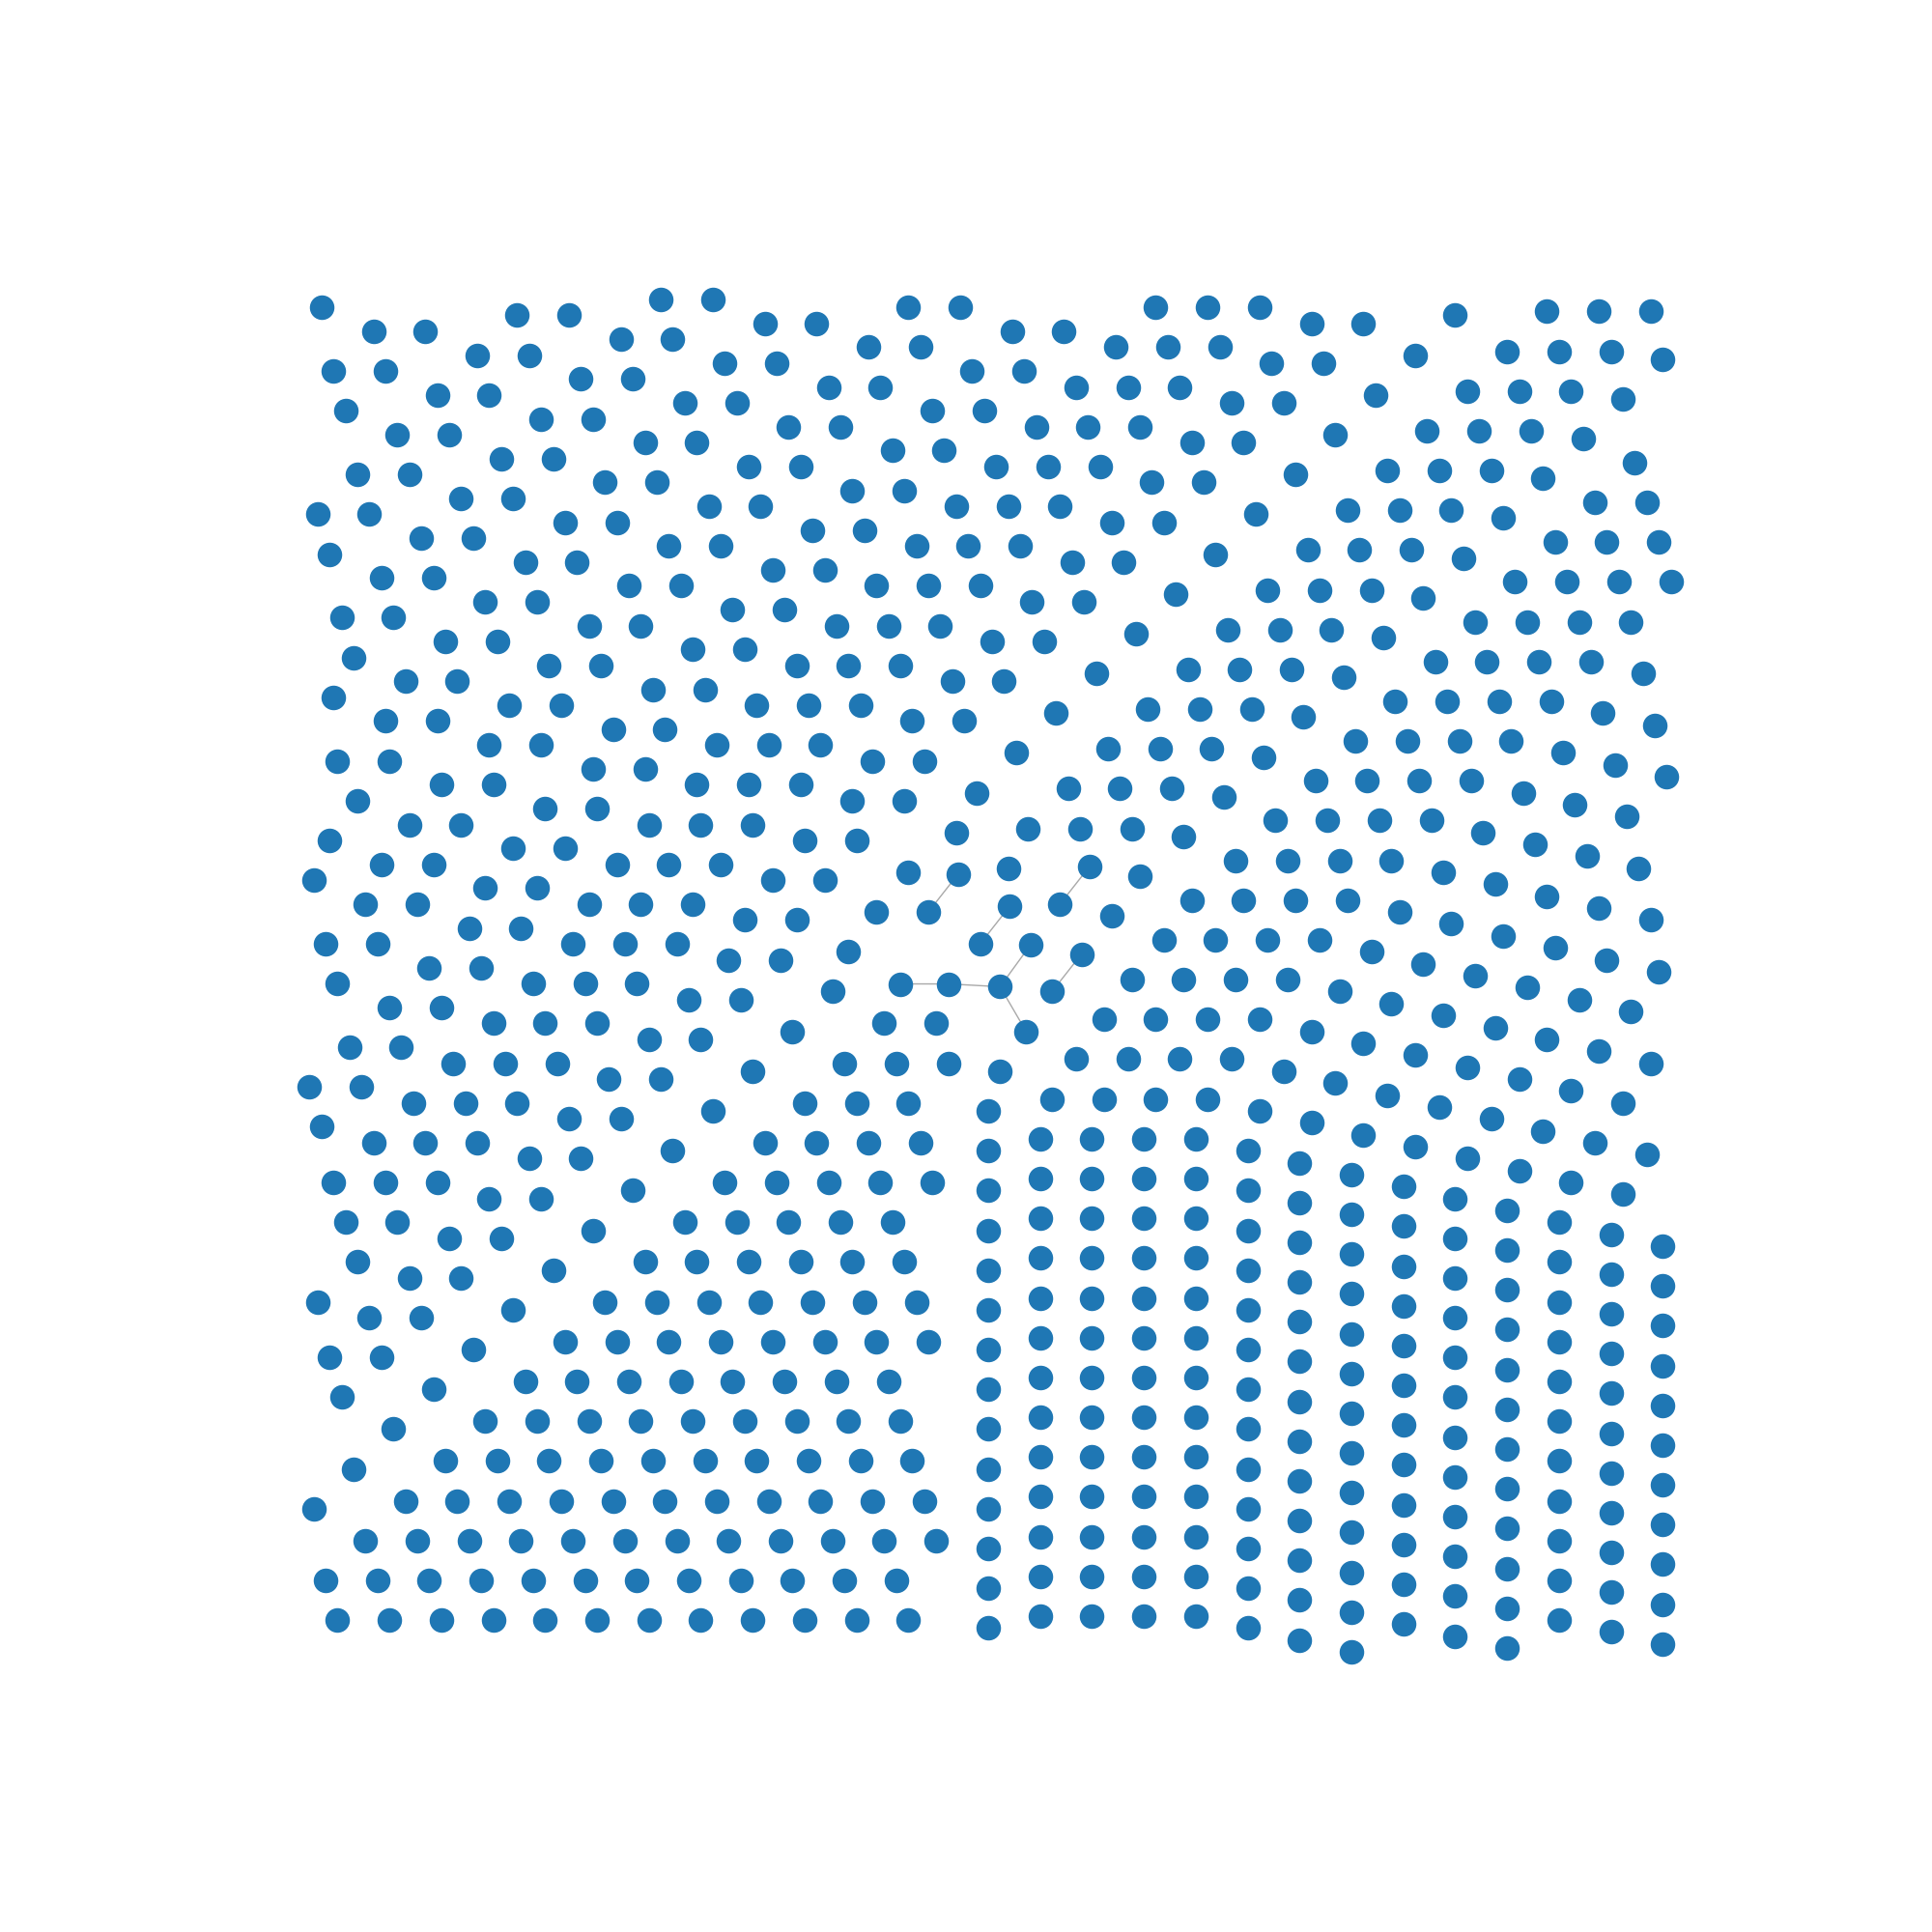
\includegraphics[width=.25\textwidth]{/files/src/.media/ego/grafo_12.png}}\hfill
    \\[\smallskipamount]
    \subfloat[$u = 12$]{
\includegraphics[width=.25\textwidth]{/files/src/.media/ego/grafo_13.png}}
    \\[\smallskipamount]
    \caption{Todos los grafos correspondientes a los diferentes umbrales, tomados a partir de las matrices de conectividad $\mathbf{C}\ \mathbf{C}^t > u$. Los números debajo de cada imagen indican el umbral utilizado.} \label{grafos_aproximados}
    %indican la cantidad de conexiones
\end{figure}




% === COMPARACION === %

\vspace{2em}
\subsection{Comparación con la red original}

% aca creo que quedaria mejor primero mencionar todos los metodos
% despues mostrar tabla resultados
% y grafico
% y despues hacer el analisis
% ej:

Nos encontramos con diferentes grafos construidos en base a los atributos en \textbf{C}. Buscamos ahora comparar nuestras aproximaciones con la red original. 

\vspace{1em}
Un primer acercamiento a este problema puede ser calcular la cantidad de \textit{posiciones coincidentes} entre las matrices de adyacencia y dividir por los elementos totales. La lógica por detrás del método es que nuestros grafos serán más similares entre sí por cada conexión y `no conexión' acertada. %Entonces, por cada 0 y 1 coincidente en nuestra aproximación y \textbf{E} nos acercaríamos más a un 100\% de similitud. 

%\vspace{1em}
Otros dos métodos de comparación posibles son la comparación de matrices por \textit{adyacencia estirada} ---donde se computa la correlación entre los vectores estirados de las matrices---, y la comparación por \textit{listas de autovalores} ---donde se computa la correlación entre los vectores ordenados de autovalores---. La correlación, por su parte, es una covarianza normalizada con valores en (-1, 1), donde números mayores indican una mayor similitud. Se describe por la siguiente fórmula:

\vspace{1em}
\begin{equation}
    Corr(x, y) = \frac{(x - \mu_{x}) \cdot (y - \mu_{y})}{\sqrt[]{(x - \mu_{x})^{2} \cdot (y - \mu_{y})^{2}}}
    \label{eq:corr}
\end{equation}

\vspace{1em}
\noindent siendo $\mu$ el valor medio de los vectores.

\vspace{1em}
\begin{figure}[!htbp]
    \begin{tabular}{ |c|c|c|c|c| } 
    \hline
    aproximación & conexiones & coincidentes & adyacencia estirada & autovalores \\
    \hline
    0            &298,799                 & 7.61\%\     & 1.25\%\               & 47.99\%\ \\
    1            &213,902                 & 32.95\%\    & 2.32\%\               & 60.86\%\ \\
    2            &127,382                 & 58.57\%\    & 2.94\%\               & 62.98\%\ \\
    3            &86,847                  & 70.99\%\    & 5.86\%\               & 75.48\%\ \\
    4            &43,091                  & 84.16\%\    & 9.61\%\               & 88.29\%\ \\
    5            &16,850                  & 91.54\%\    & 10.96\%\              & 94.28\%\ \\
    6            &5,727                   & 94.32\%\    & 9.75\%\               & 95.06\%\ \\
    7            &1,517                   & 95.21\%\    & 6.90\%\               & 92.64\%\ \\
    8            &405                     & 95.40\%\    & 4.15\%\               & 85.62\%\ \\
    9            &108                     & 95.45\%\    & 2.34\%\               & 77.52\%\ \\
    10           &36                      & 95.46\%\    & 1.35\%\               & 63.31\%\ \\
    11           &8                       & 95.46\%\    & 0.50\%\               & 55.00\%\ \\
    12           &2                       & 95.46\%\    & 0.055\%\              & 46.19\%\ \\
    13           &0                       & 95.46\%\    & 0.0\%\                & 0.0\%\  \\
    \hline
    \end{tabular} \\
    \bigskip
    \caption{Similitud elemento a elemento de las matrices de adyacencia, la primer columna representa el umbral tomado para la aproximación y la segunda la cantidad de aristas del grafo (la red `ego' original cuenta con 14.024). Las columnas siguientes miden el porcentaje de similitud respecto a \textbf{E} en función de cada método propuesto.} \label{promedio_similaridad}
\end{figure}

\vspace{1em}
\noindent \textsc{Resultados}. Como se puede observar en la figura (\ref{promedio_similaridad}.), los grafos con muy pocas conexiones (por ejemplo, para $u > 10$), tienen los valores más altos de similitud por \textit{posiciones coincidentes}, mientras que otros con cantidad de aristas similares a la red original ---como $u = 5$ o $u = 6$, que cuentan con 16,850 y 5,727 conexiones respectivamente---, parecerían ser peores aproximaciones. Esto se da por la naturaleza rala de nuestras matrices de adyacencia. La de la red `ego' \textbf{E} es de $786 \times 786$, con 617,796 elementos, y tan solo 28,048 (4.54\%) no nulos. Es decir, es rala en un 95.46\%. Es por esto que comparar elemento a elemento no prueba ser un método muy descriptivo de qué tan buena es una aproximación, ya que cualquiera con pocos elementos coincidirá en un $\sim$ 95\%.

\vspace{1em}
En la figura (\ref{grafo_correlaciones}.) se puede apreciar que se obtienen resultados considerablemente diferentes a los de nuestro primer método de comparación si se emplean los otros. En un primer lugar, siguiéndonos de la correlación entre los vectores de \textit{adyacencia estirada}, parecería que las mejores aproximaciones son las que tienen una cantidad de aristas similar a la red original ---con los umbrales $u \in [4,7]$, ver (\ref{grafos_aproximados}.)---, mientras que los grafos vacíos con umbrales más altos pasan a tener correlación nula. De la misma forma, las \textit{listas de autovalores} muestran resultados similares, donde la mayor correlación se halla con los umbrales de valores medios y decae al avanzar hacia los extremos.  


%\vspace{1em}
\begin{figure}[!htbp]
\centering
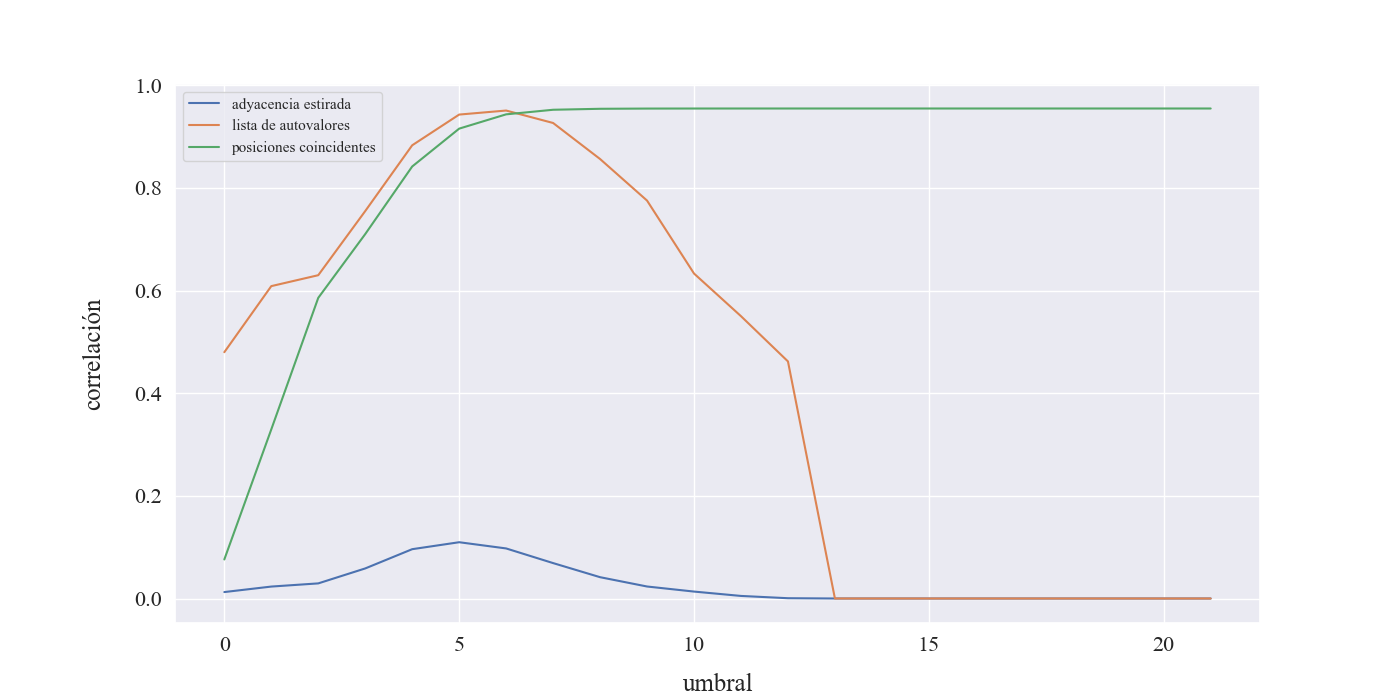
\includegraphics[scale=0.45]{/files/src/.media/ego/facebook_similaridad.png}
\caption{Similitud entre las aproximaciones y el grafo \textbf{E} para \textit{posiciones coincidentes}, \textit{adyacencia estirada} y \textit{lista de autovalores}, en función del umbral $u$.}
\label{grafo_correlaciones}
\end{figure}

\vspace{1em}
¿Cuál es, entonces, el valor para $u$ que genera la mejor aproximación? 
La figura (\ref{grafo_correlaciones}.) permite deducir que los mejores umbrales son $u = 5$ y $u = 6$. Los grafos formados bajo estas condiciones parecerían tener las mejores correlaciones con la red `ego' verdadera, sobre todo al comparar con las aproximaciones de umbrales muy bajos ($u < 2$) o muy altos ($u > 10$). Esto tiene sentido dado que mantienen una cantidad de conexiones similares al grafo original ---característica observable en la figura (\ref{grafos_aproximados}.)---, y los demás umbrales parecerían tener muy pocas aristas (hasta ninguna) o demasiadas.

Sin embargo, notamos que los resultados son considerablemente distintos a la red original. Un análisis más detallado revela que con incluso ambas de las mejores aproximaciones, $u = 5$ y $u = 6$, la cantidad de conexiones acertadas fueron tan solo 2,666 (16.87\%) y 1,106 (7.89\%) respectivamente. Aún más, la cantidad de conexiones sobrantes (existentes en la aproximación pero no en la original) fueron 14,484 y 4,621. En otras palabras, el 85.96\% de las aristas en la aproximación con $u = 5$ y el 80.69\% con $u = 6$ están de más. El método de aproximación por matriz de similaridad propuesto no fue capaz, en nuestra opinión, de capturar la estructura de la red original. 

% \vspace{2em}
% \subsection{Comparación con la red original}

% Nos encontramos con diferentes grafos construidos en base a los atributos en \textbf{C}. Buscamos ahora comparar nuestras aproximaciones con la red original. 

% Un primer acercamiento a este problema puede ser calcular la cantidad de posiciones coincidentes entre las matrices de adyacencia y dividir por los elementos totales. La lógica por detrás del método es que nuestros grafos serán más similares entre sí por cada conexión y `no conexión' acertada. Entonces, por cada 0 y 1 coincidente en nuestra aproximación y \textbf{E} nos acercaríamos más a un 100\% de similitud. 

% % aca creo que quedaria mejor primero mencionar todos los metodos
% % despues mostrar tabla resultados
% % y grafico
% % y despues hacer el analisis

% \begin{figure}[!htbp]
% \begin{equation*}
%     \begin{bmatrix}
%     0  &\%\ 7.6054231  &298.799 \\
%     1  &\%\ 32.947445  &213.902\\
%     2  &\%\ 58.570142   &127.382\\
%     3  &\%\ 70.993985    &86.847\\
%     4  &\%\ 84.162733   &43.091\\
%     5  &\%\ 91.537012   &16.850 \\
%     6  &\%\ 94.322073   &5.727\\
%     7  &\%\ 95.214277   &1.517\\
%     8  &\%\ 95.403337   &405\\
%     9  &\%\ 95.446393   &108 \\
%     10 &\%\ 95.455457   &36\\
%     11 &\%\ 95.458695   &8\\  
%     12 &\%\ 95.459342   &2\\
%     13 &\%\ 95.459990   &0\\
%     \end{bmatrix}
% \end{equation*}
% \caption{Similitud elemento a elemento de las matrices de adyacencia, la primer columna representa el umbral tomado para la aproximación y la segunda el porcentaje de elementos correctamente estimados con respecto a \textbf{E}. La tercera columna indica la cantidad de aristas del grafo; la red `ego' original cuenta con 14.024.} \label{promedio_similaridad}
% \end{figure}

% Como puede observarse en (\ref{promedio_similaridad}.), desafortunadamente, los grafos con muy pocas conexiones, como prueban ser tomando los umbrales $u > 10$, tienen de los valores más altos, mientras que otros con cantidad de aristas similares a la red original, como con $u = 5$ o $u = 6$ (16.850 y 5.727 conexiones respectivamente), parecerían ser peores aproximaciones. Esto se da por la naturaleza rala de nuestras matrices de adyacencia. La de la red `ego' \textbf{E} es de $786 \times 786$, con 617.796 elementos, y tan solo 28.048 (\% 4.54) de ellos son no nulos. Es decir, es rala en un \% 95.46. Es por esto que comparar elemento a elemento no prueba ser un método muy descriptivo de qué tan buena es una aproximación, ya que cualquiera con pocos elementos coincidirá en un $\sim$\% 95.

% \vspace{1em}

% Empleamos entonces otros dos métodos de comparación: \textit{la correlación de las matrices de adyacencia estiradas} y \textit{la correlación de las listas de autovalores}. La correlación es una covarianza normalizada con valores en (-1, 1), donde números mayores indican una mayor similitud. Esta es descrita por la siguiente fórmula:

% \begin{equation}
%     Corr(x, y) = \frac{(x - \mu_{x}) \cdot (y - \mu_{y})}{\sqrt[]{(x - \mu_{x})^{2} \cdot (y - \mu_{y})^{2}}}
% \end{equation}

% siendo $\mu$ el valor medio de los vectores.

% \vspace{1em}
% \begin{figure}[!htbp]
% \centering
% 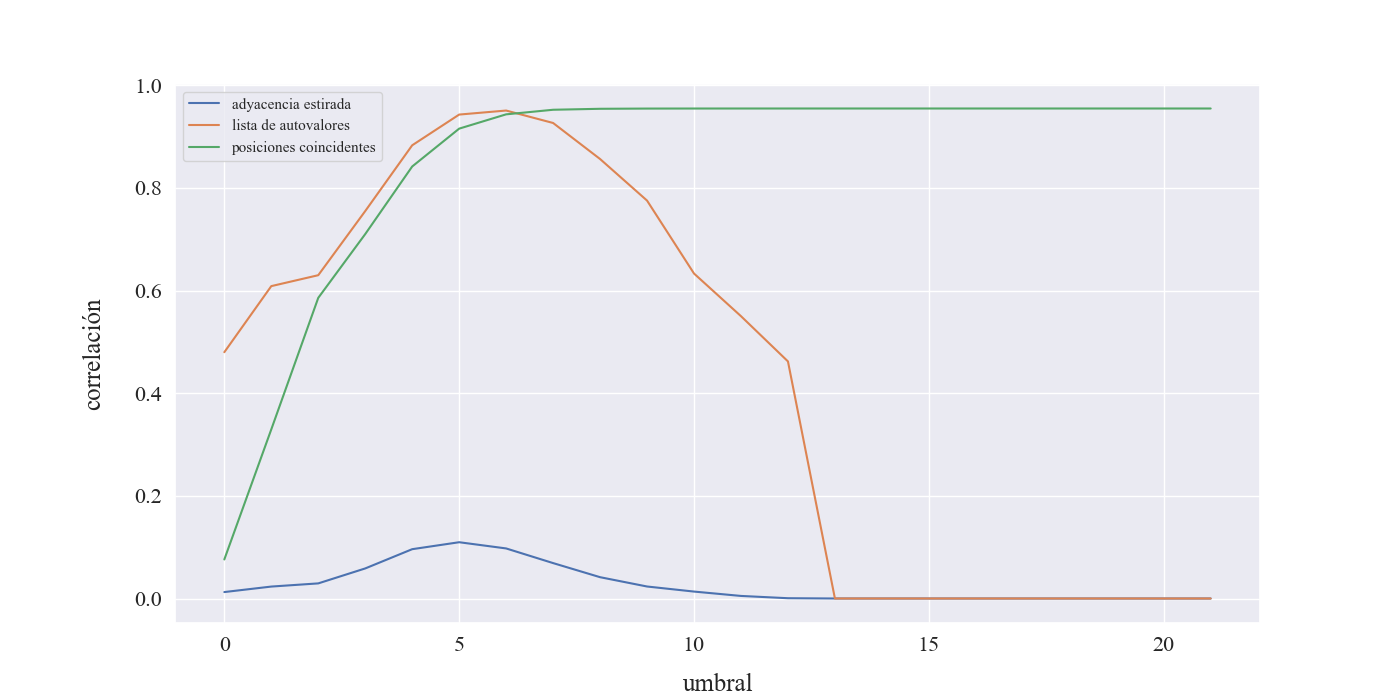
\includegraphics[scale=0.45]{/files/src/.media/ego/facebook_similaridad.png}
% \caption{Correlaciones entre matrices de adyacencia y listas de autovalores según los diferentes umbrales.}
% \label{grafo_correlaciones}
% \end{figure}

% En la figura (\ref{grafo_correlaciones}.) se puede apreciar que se obtienen resultados considerablemente diferentes a los de nuestro primer método de comparación. En un primer lugar, siguiéndonos de la correlación entre las matrices de adyacencia, parecería que las mejores aproximaciones son, razonablemente, las de cantidad de aristas similares a la red original (ver \ref{grafos_aproximados}.), con los umbrales $u \in [4,7]$, mientras que los grafos vacíos con umbrales más altos pasan a tener correlación 0. De la misma forma, analizando con los autovalores se obtienen resultados similares, donde la mayor correlación se halla con los umbrales de valores medios y decae avanzando para los extremos.  


% % === OPTIMIZACION === %

% \vspace{2em}
% \subsection{Optimización}

% ¿Cuál es entonces el valor para $u$ que genera la mejor aproximación? 
% Observando (\ref{grafo_correlaciones}.), se puede deducir que los mejores umbrales son $u = 5$ y $u = 6$. Los grafos formados bajo estas condiciones parecerían tener las mejores correlaciones con la red `ego' verdadera, sobretodo comparándolos con los de umbrales muy bajos ($u < 2$) o muy altos ($u > 10$). Esto tiene sentido dado que mantienen una cantidad de conexiones similares al grafo original, característica observable en (\ref{grafos_aproximados}.), y los demás umbrales parecerían tener muy pocas aristas (hasta ninguna) o demasiadas.


% === PCA === %

\vspace{2em}
\subsection{Análisis de componentes principales}

% Ahora bien, el conjunto describe 319 atributos distintos.
% En cada caso su significado puede variar notablemente.
% Su impacto sobre el sistema de conexiones puede diferir de tal manera que el subconjunto de atributos en consideración
% sea relevante para nuestra exploración del mismo, y tal que parte de los datos sea poco pertinente para dicho estudio.
% El Análisis de Componentes Principales (PCA) es un método que podemos aprovechar para reducir la dimensionalidad de los datos.
% Reduciendo la cantidad bajo consideración podemos obtener un conjunto de atributos que sea más relevante para la exploración del sistema de conexiones.
% PCA proyecta los datos en un espacio de menor dimensionalidad, donde los atributos son linealmente independientes, formando una base de vectores ordenados según su varianza de mayor a menor.
% Es decir, PCA organiza la información según su relevancia. Esto podria eventualmente ayudarnos a reducir la redundacía de los datos, y por ende, la cantidad de atributos que debemos considerar.
% Así se espera intercambiar un poco de precisión, deshaciendonos de información redundante, para ganar simplicidad y eficiencia computacional.

El conjunto \textbf{C} describe 319 atributos distintos, cada uno con un significado diferente\footnote{Si bien los atributos están obfuscados para mantener la privacidad de los usuarios, el dataset permite conocer de manera parcial su significado: existen atributos respecto a fechas de cumpleaños, educación, trabajo, género, nombre, apellido y lugar de residencia; por nombrar algunos. Como cada atributo es binario y múltiples refieren a las mismas cualidades, podemos suponer que no todas las combinaciones son posibles.}. %Por ejemplo, el subconjunto de atributos que designa el nombre es exclusivo dos a dos, por lo que tendrá a lo sumo un bit levantado por usuario.
Su impacto sobre nuestras aproximaciones puede diferir notablemente, de tal manera que es esperable que sólo parte de la información sea relevante para nuestra exploración.

El Análisis de Componentes Principales, \textit{PCA}, es un método que podemos aprovechar para reducir la dimensionalidad de los datos. Si consideramos al conjunto \textbf{C} como una matriz, entonces cada fila designa un usuario y cada columna un atributo. \textit{PCA} nos permite proyectar las columnas de esta matriz a un espacio de menor dimensión donde las columnas son linealmente independientes y están ordenadas según su varianza de mayor a menor.

Es decir, PCA organiza la información según su relevancia. Esto nos ayudará a reducir la redundacía de los datos, y por ende, la cantidad de atributos que debemos considerar. Así se espera intercambiar un poco de precisión, al remover información redundante, para ganar simplicidad y eficiencia computacional.

% Para lograr esto, se busca hacer un cambio de base a la matriz de datos $\textbf{C}$. 
% Y para eso vamos a diagonalizar la matriz de covarianza $\textbf{M}_x$.
% Esta contiene en su diagonal los valores de varianza de cada variable, y la covarianza (definida en \ref{eq:corr}) en el resto de sus 
% posiciones.
% La obtenemos de la siguiente manera:
% Buscamos diagonalizar esta matriz tal que, para $\textbf{M}_x = \textbf{V}\textbf{D}\textbf{V}^t$, $\textbf{V}$ contiene los autovectores de % $\textbf{M}_x$ en sus columnas.
% Permutamos las columnas de $\textbf{V}$ para que estén ordenadas de mayor a menor según los valores de la diagonal de $\textbf{D}$, los % autovalores de $\textbf{M}_x$, y obtenemos $\textbf{V}^*$. 
% La matriz resultante con base cambiada es $\textbf{C}^* = \textbf{C}\textbf{V}^*$.

\vspace{1em}
\noindent Para lograr esto, se buscará hacer un cambio de base a la matriz de datos \textbf{C}. 

\vspace{1em}
La matriz de covarianza \textbf{M}$_x$, contiene en su diagonal los valores de varianza de cada variable, y la covarianza ---definida en (\ref{eq:corr}.)--- en el resto de sus posiciones. % La obtenemos de la siguiente manera:

\vspace{1em}
\begin{equation}
	\mathbf{M}_x = \frac{\mathbf{C}^t \mathbf{C}}{n-1}
\end{equation}

\vspace{1em}
\noindent donde $n$ es la cantidad de nodos en el grafo.

\vspace{1em}
Si diagonalizamos esta matriz, tal que $\mathbf{M}_x = \mathbf{V} \mathbf{D} \mathbf{V}^t$ ---donde \textbf{V} contiene los autovectores de \textbf{M}$_x$ en sus columnas y \textbf{D} sus autovalores---, y permutamos las columnas de $\textbf{V}$ para que estén ordenadas de mayor a menor según sus autovalores asociados, obtendremos el cambio de base buscado:

\vspace{1em}
\begin{equation}
    \mathbf{C}^* = \mathbf{C} \mathbf{V}^*
\end{equation}

\vspace{1em}
\noindent donde $\mathbf{V}^* := \mathbf{V} \mathbf{P}$, con \textbf{P} una matriz de permutación.

% Podemos limitar el subconjunto de componentes principales a considerar.
% Definimos una variable $p$ como el porcentage de componentes que deseamos preservar en nuestro conjunto.

% La totalidad de los resultados obtenidos se adjuntan en el apendice (ver figuras \ref{similaridad_pca} y \ref{similaridad_pca_2}). 
% En la figura \ref{grafo_correlaciones_pca}, ilustramos nuevamente los distintos métodos de comparación para cada iteración de $p$.

\vspace{1em}
Podemos limitar el subconjunto de componentes principales a considerar. Para ello, definimos la variable $p$ como el porcentaje de componentes que deseamos preservar en nuestro conjunto. Es decir, el tamaño de la matriz $\textbf{V}^*$ va a depender de este valor.

% Así procedemos a trabajar con el valor $p$ y el umbral $u$ para estudiar nuevamente la aproximación de $\textbf{E}$. Usando $\textbf{C}^*$ construimos la matriz de similaridad e iteramos sobre el rango de umbrales.

\vspace{1em}
Procederemos a trabajar con el valor $p$ y el umbral $u$ para estudiar nuevamente las aproximaciones de $\textbf{E}$.
Usaremos $\textbf{C}^*$ para construir la matriz de similaridad e iteraremos sobre el rango de umbrales como en la sección anterior.

\vspace{2em}
\noindent \textsc{Resultados}. La totalidad de los resultados obtenidos se adjuntan en el apendice (ver figuras (\ref{similaridad_pca}.) y (\ref{similaridad_pca_2}.)). 
En la figura (\ref{grafo_correlaciones_pca}.) ilustramos nuevamente los distintos métodos de comparación para cada iteración de $p$.
Para los valores de $p$ más pequeños, el grafico difiere notablemente de los obtenidos en la sección anterior. 
Pero vemos que, como es de esperar, los resultando tienden a converger al mismo comportamiento observado previamente.

\begin{figure}[!htbp]
    \centering
    \includegraphics[scale=0.45]{/files/src/.media/ego/facebook_similaridad_pca.png}
    \caption{Similitud entre las aproximaciones y el grafo \textbf{E} para \textit{posiciones coincidentes}, \textit{adyacencia estirada} y \textit{listas de autovalores}, en función del umbral $u$, para todo $p\ \in\ \{0.4, 0.5, 0.6, 0.75, 0.8, 0.85, 0.9, 0.95, 0.99\}$.}
    \label{grafo_correlaciones_pca}
\end{figure}

\vspace{1em}
Lo más interesante es que, con menos atributos, el valor de correlación máximo difiere solo ligeramente.
Y este llega a su tope para un umbral $u$ relativamente menor.
La tabla (\ref{tabla_correlaciones_pca}.) muestra exactamente para qué valor de $u$ se alcanza la máxima correlación, en función del valor de $p$, para los métodos de \textit{adyacencia estirada} y \textit{listas de autovalores}.

\vspace{1em}
\begin{figure}[!htbp]
    \begin{tabular}{ c|c|c|c|c } 
    \hline
     & \multicolumn{2}{c}{adyacencia estirada} & \multicolumn{2}{c}{lista de autovalores} \\
    \hline
    p & u & máximo & u & máximo \\
    \hline
    0.4            &4       &10.29\%                 & 4    &89.88\%  \\
    0.5            &4       &10.18\%             & 5    &93.12\%  \\
    0.6            &5       &10.8\%                & 5     &93.05\%      \\
    0.75            &5      &10.4\%              & 6    &94.42\%     \\
    0.8            &5       &10.49\%             & 6    &94.7\%      \\
    0.85            &5      &10.81\%              & 6       &94.94\% \\
    0.9            &5       &10.96\%             & 6    &95.2\%  \\
    0.95            &5      &10.99\%              & 6      &95.26\% \\
    0.99            &5      &10.99\%               & 6      &95.06\% \\
    \hline
    \end{tabular} \\
    \bigskip
    \caption{Umbral con correlación máxima para los valores de $p$ en los métodos de \textit{adyacencia estirada} y \textit{listas de autovalores}.} \label{tabla_correlaciones_pca}
\end{figure}

% Efectivamente, para menor valores de $p$ empeora nuestra capacidad de aproximar $\textbf{E}$, pero solo levemente.
% Notar que habiendo reducido la cantidad de atributos en un 60\%, perdemos no más que 0.7\% y 5\% en la adyacencia estirada y la lista de autovalores, respectivamente.
Vemos que, para valores de $p$ menores, empeora nuestra capacidad de aproximar $\textbf{E}$, pero solo levemente.
Notamos que habiendo reducido la cantidad de atributos en un 60\%, perdemos no más que el 0.7\% y 5\% de similitud en \textit{la adyacencia estirada} y las \textit{listas de autovalores}, respectivamente.
Es decir, de necesitar el uso del PCA para reducir la dimensionalidad de los datos, los resultados obtenidos sufren meramente una leve pérdida de calidad.
También, constatamos que el rango de umbrales en los que se alcanza la máxima correlación converge a los mismos valores que en la sección anterior.
Es decir, para $u \in \{5, 6\}$.

\newpage

% potencia experimentación
\section{Experimentación extra}
% === INTRO === %

\vspace{1em}
\subsection{Una extensión del método de la potencia} \label{ap_A}

Vimos que una condición necesaria para la aplicación del método de la potencia es tener un autovalor dominante en módulo. ¿Qué sucede si esto no se cumple?

\vspace{1em}
\noindent Para simplificar el análisis separaremos en dos casos: 1. cuando hay autovalores dominantes iguales y 2. cuando no son iguales pero tienen el mismo valor absoluto.





% === 1 === %
\vspace{2em}
El método de la potencia se define por la siguiente relación de recurrencia:

\vspace{1em}
\begin{equation*} 
    b_{k+1} = \frac{\mathbf{A}b_k}{||\mathbf{A}b_k||} \qquad \forall k \in \mathbf{N}_0
\end{equation*}

\vspace{1em}
\noindent donde $b_0$ es un vector aleatorio, $||b_0||_2 = 1$.

\vspace{1em}
\noindent La demostración de convergencia de la serie definida por $\{b_k\}_{k \in \mathbb{N}_0}$ se basa en la siguiente igualdad: 

\begin{equation} \label{eq_potencia}
    b_k = \frac{\sum_{i=1}^{n} a_i \ \lambda_{i}^{k} \ x_i }{||\sum_{i=1}^{n} a_i \ \lambda_{i}^{k} \ x_i||_2}
\end{equation}

\vspace{1em}
\noindent donde $a_i := b_0^t\ x_i$, y $x_i$ es el autovector asociado al $i$-ésimo autovalor de $\mathbf{A}$ ---$\lambda_i$---, tal que $|\lambda_1| > |\lambda_2| \geq ... \geq |\lambda_n|$.

\vspace{2em}
\noindent Si suponemos, en cambio, que $|\lambda_1| = ... = |\lambda_r|$, tal que $|\lambda_1| > |\lambda_{r + 1}|$:

%\vspace{1em}
\begin{equation*} \label{eq_limite}
    b_k = \frac{\sum_{i=1}^{n} a_i \ \lambda_{i}^{k} \ x_i }{||\sum_{i=1}^{n} a_i \ \lambda_{i}^{k} \ x_i||_2} \cdot \frac{|\lambda_1|^k}{|\lambda_1|^k} 
        = \frac{\sum_{i=1}^{n} a_i \ (\frac{\lambda_{i}}{|\lambda_{1}|})^{k} \ x_i}{\frac{1}{|\lambda_{1}|^{k}}\ ||\sum_{i=1}^{n} a_i \ \lambda_{i}^{k} \ x_i||_2}
        = \frac{\sum_{i=1}^{r} a_i\ (\frac{\lambda_{i}}{|\lambda_{1}|})^{k}\ x_i + \sum_{i=r+1}^{n} a_i \ (\frac{\lambda_{i}}{|\lambda_{1}|})^{k} \ x_i }{||\sum_{i=1}^{r} a_i\ (\frac{\lambda_{i}}{|\lambda_{1}|})^{k}\ x_i + \sum_{i=r+1}^{n} a_i \ (\frac{\lambda_{i}}{|\lambda_{1}|})^{k} \ x_i ||_2}
\end{equation*}

\vspace{1em}
\noindent y tomando k par vemos que $(\frac{\lambda_{i}}{|\lambda_{1}|})^k = 1\ $ si $\ i \leq r\ $ y $\ (\frac{\lambda_{i}}{|\lambda_{1}|})^{k} \longrightarrow 0 \ \ \forall i: r + 1\ ...\ n$. Tal que $b_k$ converge a:

%\vspace{1em}
\begin{equation*}
    \lim_{k \to \infty} b_k = \frac{\sum_{i=1}^{r} a_i\ x_i }{||\sum_{i=1}^{r} a_i \ x_i||_2} = \sum_{i=1}^{r} c_i\ x_i  
\end{equation*}

\vspace{1em}
\noindent donde $c_i := a_i \cdot (||\sum_{i=1}^{r} a_i \ x_i||_2)^{-1}$. 


\newpage
\vspace{2em}
\subsubsection*{1. Método de la potencia para autovalores dominantes iguales}

Asumimos $\lambda_1 = ... = \lambda_r$

\vspace{1em}
Como $x_1$ ... $x_r$ son autovectores de $\lambda_1$, vemos que para $c_1$ ... $c_r$ arbitrarios (con la condición que exista $c_i \neq 0$):

%\vspace{1em}
\begin{equation*}
    \mathbf{A} \ \sum_{i=1}^{r} c_i\ x_i = \sum_{i=1}^{r} c_i\ \lambda_1\ x_i = \lambda_1 \sum_{i=1}^{r} c_i\ x_i
\end{equation*}

En consecuencia, sin importar quienes sean los $c_i$, se cumple que $\sum_{i=1}^{r} c_i\ x_i$ es un autovector y $\lambda_1$ es su autovalor. Esto nos permite inferir que $\lambda_1 = ... =\lambda_r$ esta asociado no solo a un autovector, sino a un subespacio de dimension $ \leq r$, ya que esta sumatoria define una combinación lineal de los $x_i$.   

\vspace{1em}
Por lo tanto, en el caso donde hay autovalores dominantes iguales, el método de la potencia converge correctamente. Este resultado lo comprobamos experimentalmente como se ve en el gráfico (\ref{fig:autovalor_repetido}.), donde se observa que el vector inicial tiende a un autovector a medida que aumenta la cantidad de iteraciones del algoritmo.

\begin{figure}[!htbp]
    \includegraphics[scale=0.45]{files/src/.media/op_autovalor_repetido.png}
    \caption{Se eligió una matriz de $20 \times 20$ con base de autovectores y dos autovalores dominantes ($\lambda_1 = \lambda_2 = 20$). En cada iteración del método de la potencia medimos el error absoluto $||20 - \bar{\lambda}||_2$. Se puede observar como, a medida que aumenta la cantidad de iteraciones, la distancia entre el autovalor y el esperado tiende a cero.}
    \label{fig:autovalor_repetido}
\end{figure}

Cabe destacar que, como $\sum_{i=1}^{r} c_i\ x_i$ es autovector para todo $c_i$ (tal que exista $c_i \neq 0$), entonces cualquier combinación lineal de los $x_i$ va a ser un autovector, y por ende hay infinitos resultados posibles con norma igual a uno ---a diferencia del caso en el que todos los autovalores son diferentes en módulo, donde hay solo dos autovectores con esta norma ---\footnote{Esto explica por qué hay que tener cuidado al comparar el autovector obtenido por el algoritmo con el que provee algún otro método, como $linalg.eig()$ de numpy.}.

\vspace{1em}
Algo interesante a notar es que, por tomar $k$ par, pudimos asumir que $signo(\lambda_1)^k = (\frac{|\lambda_{1}|}{\lambda_{1}})^k = 1$. Si no fueramos a asumir esto, observamos que en las iteraciones pares el método converge a $\sum_{i=1}^{r} c_i\ x_i$, pero en las impares, si $\lambda_1 < 0$, converge a $-\sum_{i=1}^{r} c_i\ x_i$. Ambos son autovectores válidos linealmente dependientes. Por lo que la restriccion de $k$ par no es necesaria para encontrar un autovector.

\vspace{1em}
Sin embargo, teniendo en cuenta que el método depende de la distancia entre una iteración y su consecutiva ---al comparar por tolerancia---, como en este caso el método oscila entre iteraciones pares e iteraciones impares, la distancia entre una iteración y su consecutiva no tenderá a cero. En consecuencia, de no imponer esta restricción, el método va a tener que hacer el total de las iteraciones $q$ sin poder interrumpirse antes. 




% === 2 === %

\vspace{2em}
\subsubsection*{2. Método de la potencia para autovalores diferentes pero iguales en módulo} 

Si suponemos, en cambio, que $|\lambda_1| = ... = |\lambda_r| > |\lambda_{r + 1}|$ donde los autovalores dominantes no son todos iguales, vemos si la ecuación (\ref{eq_potencia}.) efectivamente converge a un autovector:

\begin{equation*}
    \mathbf{A} \sum_{i=1}^{r} c_i\ x_i = \sum_{i=1}^{r} \mathbf{A} c_i\ x_i = \sum_{i=1}^{r} \lambda_i\ c_i\ x_i 
\end{equation*}

\vspace{2em} 
\noindent Como existe al menos un $\lambda_j$ negativo, $1 \leq j \leq r$, entonces:

\begin{equation*}
    \sum_{i=1}^{r} \lambda_i\ c_i\ x_i = \lambda_1 \sum_{i = 1,\ i \neq j}^{r} c_i\ x_i - |\lambda_j|\ c_j\ x_j = \lambda_1 (\sum_{i = 1,\ i \neq j}^{r} c_i\ x_i - c_j\ x_j)
\end{equation*}

\vspace{1em} 
\noindent pero:

\begin{equation*}
    \sum_{i=1}^{r} c_i\ x_i \neq \sum_{i = 1,\ i \neq j}^{r} c_i\ x_i - c_j\ x_j
\end{equation*}

\noindent por lo que el método de la potencia no converge a un autovector. 
Un ejemplo de esto se puede observar en el gráfico (\ref{fig:oscilante}.).

\vspace{1em}
Con este resultado en mente, observamos que en caso de computar la suma entre las últimas dos iteraciones del método de la potencia, para $k$ par lo suficientemente grande, obtendríamos lo siguiente:

% \vspace{2em}
% \noindent defino $s_i := \frac{\lambda_{i}}{|\lambda_{1}|}$. 

\begin{align*}
    \text{defino} \ s_i :&= \frac{\lambda_{i}}{|\lambda_{1}|} \\
    b_k = \frac{\sum_{i=1}^{r} a_i \ s_i^k \ x_i }{||\sum_{i=1}^{r} a_i \ s_i^k \ x_i||_2} &= \frac{\sum_{i: \lambda_i > 0}^{r} a_i \ x_i  + \sum_{i: \lambda_i < 0}^{r} a_i \ x_i}{||\sum_{i: \lambda_i > 0}^{r} a_i \ x_i  + \sum_{i: \lambda_i < 0}^{r} a_i \ x_i||_2} \\\\
    b_{k+1} = \frac{\sum_{i=1}^{r} a_i \ s_i^{k+1} \ x_i }{||\sum_{i=1}^{r} a_i \ s_i^{k+1} \ x_i||_2} &= \frac{\sum_{i: \lambda_i > 0}^{r} a_i \ x_i - \sum_{i: \lambda_i < 0}^{r} a_i \ x_i}{||\sum_{i: \lambda_i > 0}^{r} a_i \ x_i  - \sum_{i: \lambda_i < 0}^{r} a_i \ x_i||_2} \\\\
    \text{Como los $x_i$ son ortogonales en}& \text{tre sí se puede probar por pitágoras que:} \\ 
    ||\sum_{i: \lambda_i > 0}^{r} a_i \ x_i  - \sum_{i: \lambda_i < 0}^{r} a_i \ x_i||_2 &=  \ ||\sum_{i: \lambda_i > 0}^{r} a_i \ x_i  + \sum_{i: \lambda_i < 0}^{r} a_i \ x_i||_2 \\
    \text{defino} \ d_i :&= (||\sum_{i: \lambda_i > 0}^{r} a_i \ x_i  + \sum_{i: \lambda_i < 0}^{r} a_i \ x_i||_2)^{-1} \cdot a_i \\
    b_{k+1} + b_k = \sum_{i: \lambda_i > 0}^{r} d_i \ x_i - \sum_{i: \lambda_i < 0}^{r} d_i \ x_i \ &+ \sum_{i: \lambda_i > 0}^{r} d_i \ x_i + \sum_{i: \lambda_i < 0}^{r} d_i \ x_i = \ 2 \sum_{i: \lambda_i > 0}^{r} d_i \ x_i \\
\end{align*}

Es decir, estaríamos en la condición de la subsección anterior, por lo que  queda demostrado que en caso de que el autovalor dominante este repetido en módulo, basta con computar la suma entre 2 iteraciones consecutivas que convergería al autovector asociado a $\lambda_1$.

\begin{figure}[!htbp]
    \includegraphics[scale=0.45]{files/src/.media/op_oscilante.png}
    \caption{Se eligió una matriz de $20 \times 20$ con base de autovectores y dos autovalores dominantes $\lambda_1 = 20$, $\lambda_2 = -20$. Además se seleccionó un vector aleatorio constante normalizado $v$. En cada iteración del método de la potencia calculamos la distancia $||v - y_k||_2$. Se puede apreciar como $v$ oscila entre las iteraciones pares e impares.}
    \label{fig:oscilante}
\end{figure}

\vspace{1em}
Observamos que se podría calcular la resta entre $b_{k+1}$ y $b_k$ para obtener otro autovector: el asociado a $\sum_{i: \lambda_i < 0}^{r} d_i\ x_i$. Es decir, podríamos obtener dos autovectores en un sólo llamado al método de la potencia. Como el método de la deflacíon asume que el método de la potencia encuentra de a un solo autovector por vez, decidimos no complejizar el algoritmo para aprovechar este caso puntual.



\newpage
% === 3 === %

\vspace{2em}
\subsubsection*{3. El nuevo método} Con este resultado en mente planteamos el siguiente algoritmo como alternativa para el método de la potencia \textit{monte carlo}.

\vspace{1em}
\lstinputlisting[mathescape=true, escapechar=@, language=pseudo, label=potencia_modificada, caption={Pseudocódigo para una versión alternativa del \textit{método de la potencia}. El mismo soluciona el caso de autovalores en módulo repetidos.}]{files/src/.code/potencia_modificada.pseudo}

\vspace{1em}
Dada una matriz simétrica sin restricciones extra, este algoritmo permite calcular sus $k$ autovalores ---y vectores asociados--- no nulos. Esto permite relajar de manera considerable las restricciones del método original.

\newpage

% conclusiones
\section{Conclusiones}
\vspace{2em}

En este trabajo, habiendo implementado el método de la potencia y experimentado con él, observamos distintos problemas en el mismo, tales como el error numérico o su incapacidad de calcular los autovectores de las matrices con autovalores repetidos en valor absoluto. Es por esto que experimentamos con diferentes modificaciones al método propuesto para abarcar todos los casos posibles. Además, propusimos optimizaciones al algoritmo, como lo es ir de a pasos pares, para acortar la cantidad de iteraciones que requería para converger. 

\vspace{1em}
Luego, con la implementación del método, comenzamos a experimentar con distintos casos de uso práctico. Por un lado, en el apartado del \textit{Club de Karate}, vimos la utilidad de la centralidad de autovector y conectividad algebraica en la matriz laplaciana para evaluar las distintas características de una red. 

\vspace{1em}
Por otro lado, el análisis de las red `Ego' de Facebook nos permitió experimentar con diferentes aproximaciones de las mismas, evaluando sus similitudes a la original y determinando cuáles fueron las mejores. También, recurrimos al análisis de componentes principales (PCA) para reducir la dimensionalidad del conjunto de datos, y observamos los resultados sobre distintos rangos de la matriz de covarianza. Afirmamos de esta manera la posibilidad de aplicar una reducción, a bajo costo de calidad en nuestra predicción.

\vspace{1em}
En conclusión, observamos que el cálculo de autovalores y autovectores no es una tarea sencilla, pero a su vez posee una gran utilidad para el estudio de matrices. Nos brindan información de la estructura subayacente de los datos y su comportamiento, por lo que son imprescindibles para el análisis de toda clase de problemas.

\newpage

% apendice
\section{Apéndice}

\vspace{1em}
\begin{figure}[!htbp]
    \scalebox{0.7}{
        \begin{tabular}{ |c|c|c|c|c|c|c| } 
        \hline
        p & atributos & u & conexiones & coincidentes & adyacencia estirada & autovalores \\
        \hline
        0.5             &12             &0            &229,602                 & 28.19\%\     & 1.73\%\               & 58.84\%\ \\
        0.5             &12             &1            &133,807                 & 56.57\%\     & 2.37\%\               & 60.61\%\ \\
        0.5             &12             &2            &95,224                 & 68.42\%\     & 5.12\%\               & 74.32\%\ \\
        0.5             &12             &3            &49,381                 & 82.28\%\     & 8.86\%\               & 86.65\%\ \\
        0.5             &12             &4            &20,125                 & 90.58\%\     & 10.18\%\               & 92.33\%\ \\
        0.5             &12             &5            &6,716                 & 94.04\%\     & 9.15\%\               & 93.12\%\ \\
        0.5             &12             &6            &1,727                 & 95.14\%\     & 6.08\%\               & 89.81\%\ \\
        0.5             &12             &7            &393                 & 95.4\%\     & 3.45\%\               & 80.9\%\ \\
        0.5             &12             &8            &95                 & 95.44\%\     & 1.66\%\               & 73.24\%\ \\
        0.5             &12             &9            &24                 & 95.46\%\     & 1.22\%\               & 62.23\%\ \\
        \hline
        0.75             &45             &0            &298,220                 & 7.79\%\     & 1.34\%\               & 49.38\%\ \\
        0.75             &45             &1            &212,612                 & 33.34\%\     & 2.36\%\               & 62.21\%\ \\
        0.75             &45             &2            &125,175                 & 59.22\%\     & 2.97\%\               & 64.39\%\ \\
        0.75             &45             &3            &84,766                 & 71.6\%\     & 5.85\%\               & 76.71\%\ \\
        0.75             &45             &4            &41,516                 & 84.57\%\     & 9.36\%\               & 88.34\%\ \\
        0.75             &45             &5            &15,922                 & 91.73\%\     & 10.4\%\               & 93.74\%\ \\
        0.75             &45             &6            &5,274                 & 94.4\%\     & 9.07\%\               & 94.42\%\ \\
        0.75             &45             &7            &1,342                 & 95.24\%\     & 6.36\%\               & 91.53\%\ \\
        0.75             &45             &8            &333                 & 95.41\%\     & 3.5\%\               & 83.16\%\ \\
        0.75             &45             &9            &89                 & 95.45\%\     & 1.74\%\               & 75.06\%\ \\
        0.75             &45             &10            &28                 & 95.46\%\     & 0.94\%\               & 59.58\%\ \\
        0.75             &45             &11            &8                 & 95.46\%\     & 0.81\%\               & 52.95\%\ \\
        0.75             &45             &12            &1                 & 95.46\%\     & 0.04\%\               & 34.07\%\ \\
        \hline
        0.8             &60             &0            &298,611                 & 7.66\%\     & 1.26\%\               & 48.59\%\ \\
        0.8             &60             &1            &213,405                 & 33.09\%\     & 2.31\%\               & 61.25\%\ \\
        0.8             &60             &2            &126,336                 & 58.87\%\     & 2.89\%\               & 63.2\%\ \\
        0.8             &60             &3            &85,825                 & 71.28\%\     & 5.82\%\               & 76.06\%\ \\
        0.8             &60             &4            &42,266                 & 84.36\%\     & 9.35\%\               & 88.29\%\ \\
        0.8             &60             &5            &16,324                 & 91.63\%\     & 10.49\%\               & 93.97\%\ \\
        0.8             &60             &6            &5,488                 & 94.35\%\     & 9.22\%\               & 94.7\%\ \\
        0.8             &60             &7            &1,423                 & 95.23\%\     & 6.53\%\               & 91.99\%\ \\
        0.8             &60             &8            &364                 & 95.4\%\     & 3.65\%\               & 84.08\%\ \\
        0.8             &60             &9            &101                 & 95.45\%\     & 2.01\%\               & 76.82\%\ \\
        0.8             &60             &10            &34                 & 95.46\%\     & 1.25\%\               & 63.04\%\ \\
        0.8             &60             &11            &8                 & 95.46\%\     & 0.5\%\               & 55.0\%\ \\
        0.8             &60             &12            &1                 & 95.46\%\     & 0.04\%\               & 34.07\%\ \\
        \hline
        0.85             &81             &0            &298,815                 & 7.6\%\     & 1.22\%\               & 48.0\%\ \\
        0.85             &81             &1            &213,850                 & 32.96\%\     & 2.28\%\               & 60.65\%\ \\
        0.85             &81             &2            &127,188                 & 58.61\%\     & 2.88\%\               & 62.59\%\ \\
        0.85             &81             &3            &86,783                 & 71.0\%\     & 5.81\%\               & 75.42\%\ \\
        0.85             &81             &4            &42,996                 & 84.17\%\     & 9.49\%\               & 88.21\%\ \\
        0.85             &81             &5            &16,780                 & 91.54\%\     & 10.81\%\               & 94.16\%\ \\
        0.85             &81             &6            &5,686                 & 94.32\%\     & 9.48\%\               & 94.94\%\ \\
        0.85             &81             &7            &1,498                 & 95.21\%\     & 6.74\%\               & 92.41\%\ \\
        0.85             &81             &8            &395                 & 95.4\%\     & 3.88\%\               & 84.79\%\ \\
        0.85             &81             &9            &106                 & 95.45\%\     & 2.2\%\               & 77.33\%\ \\
        0.85             &81             &10            &35                 & 95.46\%\     & 1.23\%\               & 63.26\%\ \\
        0.85             &81             &11            &8                 & 95.46\%\     & 0.5\%\               & 55.0\%\ \\
        0.85             &81             &12            &3                 & 95.46\%\     & 0.43\%\               & 47.93\%\ \\
        \hline
        \end{tabular}
    }
    \bigskip
    \caption{Tabla de similitud. Equivalente a la figura (\ref{promedio_similaridad}.), para distintos valores de $p$. `Atributos' refiere a la cantidad de datos preservados después de la transformación. No incluye umbrales sin conexiones. Continúa en la figura (\ref{similaridad_pca_2}.).} \label{similaridad_pca}
\end{figure}


\newpage
\begin{figure}[!htbp]
    \scalebox{0.7}{
        \begin{tabular}{ |c|c|c|c|c|c|c| } 
        \hline
        p & atributos & u & conexiones & coincidentes & adyacencia estirada & autovalores \\
        \hline
        0.9             &110             &0            &298,805                 & 7.6\%\     & 1.25\%\               & 48.01\%\ \\
        0.9             &110             &1            &213,934                 & 32.94\%\     & 2.31\%\               & 60.94\%\ \\
        0.9             &110             &2            &127,396                 & 58.56\%\     & 2.92\%\               & 62.97\%\ \\
        0.9             &110             &3            &86,886                 & 70.98\%\     & 5.85\%\               & 75.53\%\ \\
        0.9             &110             &4            &43,122                 & 84.15\%\     & 9.59\%\               & 88.34\%\ \\
        0.9             &110             &5            &16,901                 & 91.52\%\     & 10.96\%\               & 94.34\%\ \\
        0.9             &110             &6            &5,773                 & 94.31\%\     & 9.78\%\               & 95.2\%\ \\
        0.9             &110             &7            &1,546                 & 95.21\%\     & 7.03\%\               & 92.86\%\ \\
        0.9             &110             &8            &416                 & 95.4\%\     & 4.12\%\               & 85.64\%\ \\
        0.9             &110             &9            &110                 & 95.45\%\     & 2.23\%\               & 77.06\%\ \\
        0.9             &110             &10            &37                 & 95.46\%\     & 1.32\%\               & 63.46\%\ \\
        0.9             &110             &11            &8                 & 95.46\%\     & 0.5\%\               & 55.0\%\ \\
        0.9             &110             &12            &3                 & 95.46\%\     & 0.43\%\               & 47.93\%\ \\
        \hline
        0.95             &157             &0            &298,831                 & 7.6\%\     & 1.26\%\               & 48.1\%\ \\
        0.95             &157             &1            &213,950                 & 32.93\%\     & 2.33\%\               & 61.01\%\ \\
        0.95             &157             &2            &127,428                 & 58.56\%\     & 2.94\%\               & 63.04\%\ \\
        0.95             &157             &3            &86,902                 & 70.98\%\     & 5.87\%\               & 75.55\%\ \\
        0.95             &157             &4            &43,155                 & 84.15\%\     & 9.62\%\               & 88.38\%\ \\
        0.95             &157             &5            &16,900                 & 91.53\%\     & 10.99\%\               & 94.38\%\ \\
        0.95             &157             &6            &5,770                 & 94.31\%\     & 9.8\%\               & 95.26\%\ \\
        0.95             &157             &7            &1,544                 & 95.21\%\     & 6.99\%\               & 92.9\%\ \\
        0.95             &157             &8            &412                 & 95.4\%\     & 4.27\%\               & 85.79\%\ \\
        0.95             &157             &9            &114                 & 95.45\%\     & 2.41\%\               & 78.33\%\ \\
        0.95             &157             &10            &36                 & 95.46\%\     & 1.35\%\               & 63.31\%\ \\
        0.95             &157             &11            &9                 & 95.46\%\     & 0.75\%\               & 56.17\%\ \\
        0.95             &157             &12            &2                 & 95.46\%\     & 0.06\%\               & 46.19\%\ \\
        \hline
        0.99             &237             &0            &298,804                 & 7.6\%\     & 1.26\%\               & 48.03\%\ \\
        0.99             &237             &1            &213,910                 & 32.95\%\     & 2.33\%\               & 60.88\%\ \\
        0.99             &237             &2            &127,386                 & 58.57\%\     & 2.94\%\               & 62.99\%\ \\
        0.99             &237             &3            &86,858                 & 70.99\%\     & 5.86\%\               & 75.5\%\ \\
        0.99             &237             &4            &43,097                 & 84.16\%\     & 9.61\%\               & 88.3\%\ \\
        0.99             &237             &5            &16,861                 & 91.54\%\     & 10.99\%\               & 94.32\%\ \\
        0.99             &237             &6            &5,730                 & 94.32\%\     & 9.78\%\               & 95.08\%\ \\
        0.99             &237             &7            &1,524                 & 95.22\%\     & 6.99\%\               & 92.72\%\ \\
        0.99             &237             &8            &406                 & 95.4\%\     & 4.19\%\               & 85.64\%\ \\
        0.99             &237             &9            &109                 & 95.45\%\     & 2.32\%\               & 77.83\%\ \\
        0.99             &237             &10            &36                 & 95.46\%\     & 1.35\%\               & 63.31\%\ \\
        0.99             &237             &11            &8                 & 95.46\%\     & 0.5\%\               & 55.0\%\ \\
        0.99             &237             &12            &2                 & 95.46\%\     & 0.06\%\               & 46.19\%\ \\
        \hline
        \end{tabular}
    }
    \bigskip
    \caption{Continuación de la figura (\ref{similaridad_pca}.).} \label{similaridad_pca_2}
\end{figure}

\vspace{1em}

\newpage
% bibliografia - requiere que haya citas
\bibliographystyle{plain}
\bibliography{files/citations.bib}
%\newpage

\end{document}
